%%%%%%%%%%%%%%%%%%%%%%% file template.tex %%%%%%%%%%%%%%%%%%%%%%%%%
%
% This is a general template file for the LaTeX package SVJour3
% for Springer journals.          Springer Heidelberg 2010/09/16
%
% Copy it to a new file with a new name and use it as the basis
% for your article. Delete % signs as needed.
%
% This template includes a few options for different layouts and
% content for various journals. Please consult a previous issue of
% your journal as needed.
%
%%%%%%%%%%%%%%%%%%%%%%%%%%%%%%%%%%%%%%%%%%%%%%%%%%%%%%%%%%%%%%%%%%%
%
\let\nofiles\relax
% \documentclass{svjour3}                     % onecolumn (standard format)
% \documentclass[smallcondensed]{svjour3}     % onecolumn (ditto)
\documentclass[smallextended]{svjour3}       % onecolumn (second format)
% \documentclass[twocolumn]{svjour3}          % twocolumn
%
\smartqed  % flush right qed marks, e.g. at end of proof
%
\usepackage{graphicx}
\usepackage{natbib}
\usepackage{ulem}
%
% \usepackage{mathptmx}      % use Times fonts if available on your TeX system
%
% insert here the call for the packages your document requires
%\usepackage{latexsym}
% etc.
%
% please place your own definitions here and don't use \def but
% \newcommand{}{}
%
% Insert the name of "your journal" with
% \journalname{myjournal}
%
\usepackage{enumerate}
\usepackage{float}
\usepackage{makecell}
\usepackage{times}
\usepackage{amsmath}% cases equation
\usepackage{algorithm} % code
\usepackage{algorithmic} %code
\usepackage{subcaption} %subfigure
\usepackage{amssymb} % special symbol
\usepackage{caption} % caption settings for fig, table...
\usepackage{indentfirst} 
\usepackage[dvipsnames]{xcolor}
% \usepackage{todonotes}
\usepackage{marginnote}
% \usepackage[utf8]{inputenc}
% \usepackage[english]{babel}
% \usepackage{geometry}

\captionsetup[figure]{name={Fig.},labelsep=space,labelfont=bf,font=small} 
\captionsetup[table]{name={Table},labelsep=space,labelfont=bf,font=small}
\captionsetup[algorithm]{name={Algorithm},labelsep=space,labelfont=bf,font=small}
\newtheorem{mypro}[proposition]{Proposition}
% \theoremstyle{definition} \newtheorem*{myproof}{Proof}
\setlength {\marginparwidth }{6cm}
\begin{document}

\title{Modeling Bus Bunching along a Common Line Corridor considering Passenger Transfer Behavior and Capacity Constraint}
\subtitle{Full Paper}

%\titlerunning{Short form of title}        % if too long for running head

\author{First Author         \and
        Second Author %etc.
}

%\authorrunning{Short form of author list} % if too long for running head

\institute{F. Author \at
              first address \\
              Tel.: +XXX-XX-XXXXXX\\
              Fax: +XXX-XX-XXXXXX\\
              \email{fauthor@example.com}           %  \\
%             \emph{Present address:} of F. Author  %  if needed
           \and
           S. Author \at
              second address
}



\maketitle

\begin{Abstract}
Bus bunching problem is a longstanding problem in public transport operations
and degrades the efficiency and quality of transit services. 
The development of an effective scheme to mitigate its adverse impacts relies on understanding the bus movement and depicting bus trajectories. 
Existing methods inadequately address two issues, namely, capacity constraint and passengers travel behavior in multi-line scenarios.
Thus, this study develops a method that captures passengers' travel behaviors including boarding, alighting, failing to board and transfer, considering capacity constraint, and a corresponding algorithm to determine bus trajectories.
Meanwhile, a transfer-based equilibrium is proposed to describe passengers' transfer behaviors in multi-line scenarios and formulated as a Variational Inequality problem.
Numerical examples are conducted to examine the effects of passenger travel behavior and capacity constraint on the propagation of bus bunching.
\textcolor{red}{"distributed bus line?","enhance?"}
It is found that the propagation of bus bunching from a disturbed bus line to an undisturbed bus line via the common corridor is enhanced because of the presence of transfer passengers. 
This implies that \textcolor{red}{motivating passengers }. 
Furthermore, sensitivity tests show that using small buses with low capacity could help to restore regular bus services once bus bunching occurs as bus dwell times are constrained to mitigate bus bunching propagation.
\textcolor{red}{add the smaller bus capacity also in the conclusion section}

\keywords{Bus bunching \and Common line problem \and Public transport \and Capacity constraint \and Passenger transfer.}
% \PACS{PACS code1 \and PACS code2 \and more}
% \subclass{MSC code1 \and MSC code2 \and more}
\end{abstract}

\section{Introduction}
\label{intro}
% Public transport plays an important role in the urban transportation system. 
In the last decade, more and more attention has been attracted on providing high-quality public transport services with the advocate of sustainable urban mobility.
However, maintaining a reliable and efficient bus operation is very challenging and the unbalance between the transit supply and passenger demand is commonly observed in public transport operations.
Indeed, bus services in many metropolitan areas are criticized for being inefficient, irregular, and overcrowded.
Low-quality bus services frustrate passengers and lead to a reduction in bus modal split rate especially for commuters.
For example, the number of annual passenger trips of public transport in Beijing dropped from 4.84 billion in 2013 to 3.13 billion in 2019, while the number of motor trips increased from 5.44 million to 6.365 million during the same period.
\footnote[1]{Data from the \textit{2020 Beijing Transport Developm annual report}}
% \reversemarginpar \marginnote{\textcolor{red}{1} Maybe find some data/research paper to justify the statement}
% However, bus bunching is longstanding in bus operation and degrades the reliability and effectiveness of transit service.
One of the crucial problems in public transport operations is the bus bunching problem, which is commonly described as a phenomenon of schedule disruption and headway irregularity in bus operation.
The problem concerns both passengers and transit agencies \citep{1964Nwell,1972Osuna,2008Hollander,2016Verbich}.
From the passengers' perspective, the bus bunching problem is intuitively observed as the incidental phenomenon that 
two or more buses arrive at a stop with headways significantly different than designed. 
It may lead shorter waiting time for some passengers while longer waiting time for others. 
Either way, passengers' travel plan and route choice could be affected. 
From the operators' perspective, bus bunching degrades the reliability and effectiveness of transit services, which would require the operator to raise the operation cost to maintain the supply level. 
Nevertheless, the bus bunching problem is a natural characteristic of public transport operations. This is because the public transport system suffers inevitable endogenous uncertainties and exogenous random disturbances that leads to uncertain bus travel time and bus delays; and whenever a delay occurs, the delayed bus picks more passengers, while its following bus picks less, enlarging the variability of bus headway. 
Therefore, without countermeasures, once bus bunching occurs, a conventional bus operation can hardly recover to the designed schedule or expected headway especially in peak hours when passenger demand and service frequency are both high \citep{1964Nwell,2001Hickman,2009Daganzo}.
The occurrence of bus bunching is mainly attributed to two factors, one is the uncertain travel time and the other is the fluctuate passenger demands that induce the uncertainties of bus dwell times at stops \citep{2015Fonzone}.
Accordingly, the resolve of the bus bunching problem requires understanding and modeling both bus movements and passenger behaviors within the bus operation.
Although several models have been proposed in the literature to analyse bus bunching and develop methods to  mitigate its adverse impacts, most of the existing studies focused on oversimplified scenarios in which some critical issues like passenger transfer behavior and capacity constraint were not well addressed.
In what follows, the literature in bus bunching are reviewed, and the research gap is identified.
% \section{Literature review}\label{Literature review}
In the light of the seminal work about bus bunching of \cite{1964Nwell}, 
extensive researches on control schemes of encountering bus bunching have been conducted.
% \subsection{Control schemes to mitigate bus bunching}
Earlier literature focused on developing static control schemes in the planing level, 
such as adding slacks to schedules according to so-called static schedule-based holding schemes 
\citep{1989Abkowitz,2001Eberlein}.% \marginnote{\textcolor{red}{(Newell, 1974)}}[0cm]
Since the technique of intelligent transport and control system has been developing rapidly from the beginning of this century, various dynamic bus control schemes taking the advantage of real-time information have been proposed.
The real-time control strategies can be generally categorized into two groups \citep{2015Ibarra-Rojas}.
1) Station strategies such as holding strategy, stop-skipping strategy and boarding limit strategy.
2) Inter-station control strategies such as coordinated speed adjustment and traffic signal priority.
Among these dynamic control strategies, holding strategy is the most practical strategy in application \citep{2013Cats,2001Eberlein}
% \marginnote{\textcolor{red}{(Cats et al., 2011)}}[0cm]. 
The efficiency of dynamic holding strategy has been testified in literature
\citep{2009Daganzo,2011Xuan,2012ABartholdi,2015Argote-Cabanero}.
A critical shortcoming of holding control is that it results in longer bus dwell times and lower travel speed.
\textcolor{red}{"tiny bus bunching?"}
Moreover holding strategies deal the tiny bus bunching well while fails to work in severe schedule disruption.
Therefore, other novel strategies were proposed to make up for the insufficiency of holding strategies and outperform them in specific conditions. For example, stop-skipping strategy \citep{2003Fu,2005Sun} 
and substitution strategy \citep{2018Petit,2019Petit} are investigated to recover from severe schedule disruption. Coordinated speed adjustment \citep{2011Daganzo} is based on bus dedicated lane premise to reduce the extra dwell time and maintain an acceptable operating speed.
% \marginnote{\textcolor{red}{(Daganzo and Pilachowski, 2009, 2011)}}[0cm]

Most of the existing studies focus on investigating the bus bunching problem in a single line scenario to simplify the formulation and analyses. However, in practice, many urban corridors are served by multiple bus lines. This requires modelling and determining passengers routing behaviors among the multiple bus lines, known as the common line problem \citep{2015Argote-Cabanero}. 
Only in the recent five years, several researches investigated bus bunching in multi-line scenarios \citep{2015Carlos,2015Argote-Cabanero,2016Sun,2019Petit,2020Seman}. %\marginnote{\textcolor{red}{Sun?}}[0cm]

\textcolor{red}{
1. in the next sentence, "their work" ??
2. following the previous sentence, describe the literature 
3. then summarize again, say, "the above only consider transfer or capacity, and none of these consider two aspects simultaneously"
4. the literature review is not solid, "event simulation, bus motion, performence meaures"
}
For example, Hernández et al. (2015) developed an optimization model for holding strategy on multi-line system.
They considered capacity constraint but ignored transfer behavior. Schmöcker et al. (2016) investigated the effects of common stops on bus bunching with and without overtaking issue. 
Their results show that the presence of common stops has positive effects when overtaking is possible.
They focused on the equilibrium queuing behavior but ignored the passenger transfer behavior and the capacity constraint. 
Petit et al. (2019) developed an optimization model to implement substitution strategy 
in a multiline system, but assumed that different bus lines were independent of each other for the sake of simplicity. 

Nevertheless, neither of the above works considers bus capacity and passengers' transfer behavior simultaneously. Therefore, this study develops a method to close the research gap. 
To be more specific, the capacity is incorporated into a set of equations for characterizing passengers' movement, including boarding, alighting, and transfer. 
To determine the number of transfer passengers, a transfer-based equilibrium is proposed, in the light of the approach-based transit assignment model developed in \citep{2016Sun,2013Long,2014Szeto,2016Jiang}. 
The transfer-based equilibrium is different from the approach-based transit assignment in the sense that it determines the number of passengers transferring to a particular bus in a schedule-based transit network.
Meanwhile, our method is different from \citep{2016Sun,2017Wu}, since their model focuses on the boarding behavior and bus overtaking is allowed, while ours focuses on the transfer behaviors and forbits bus overtaking, which is a common practice in the bus system operated in Beijing. \textcolor{red}{need to check, beijing operation. maybe ok}

% \textrm{(Osuna and Newell, 1972; Newell, 1974; Barnett, 1974; Delgado et al., 2009, 2012; Zhao et al., 2016)}.
% The boarding limit strategy to control bus dwell time
% and traffic signal priority (Liu et al., 2003; Ling and Shalaby, 2004; Estrada et al., 2016)
% More recently, some novel schemes like overtaking \textrm{(Schmöcker et al., 2016; Wu et al., 2017)} 
% \subsection{Related literature about multi-line systems}
% but most of them only consider single transit line scenarios. 
% \subsection{Passenger behavior}
\textcolor{red}{What's more is not very formal, the followng graph could be deleted}
What's more, except two papers involved distributed passenger boarding behavior when bus overtaking was allowed \citep{2016Sun,2017Wu}
most of the existing studies on bus bunching and control strategies ignored passenger equilibrium behavior under the control strategies.
In fact, passenger behaviors affect the propagation of bus bunching and the performance of control strategies.
Therefore, we focus on the transfer behavior and formulate a transfer-based equilibrium to simulate the routing result of transfer passengers.
and divert some methodologies and concepts such as fail-to-board probability and MSA algorithm in formulating transfer cost function and searching for equilibrium solutions.

To sum up, the main contributions of this study include:
\textcolor{red}{the last contribution may be weak, but i normally seperate the contribution between, methodology and results}
\begin{enumerate}
    \item Developing a method for analysing the bus bunching problem considering passenger transfer behavior and capacity constraint simultaneously in multi-line scenarios;
    \item Proposing a transfer-based equilibrium formulation to determine the number of transfer passengers;
    \item Developing an algorithm that integrates a event-based simulation and method of successive averages 
     for obtaining bus trajectories and passengers' routing behavior;
    \item Devising a novel indicator to measure the impact of the bus bunching problem in both temporal and spatial dimensions.
    \item Conducting numerical experiments to demonstrate the effect of capacity constraint and passengers' transfer behavior on the propagation of bus bunching and the performance of the proposed algorithm.
\end{enumerate}

\textcolor{red}{remark: the literature on "event-based" simulation may be reviewed}
The remaining of the paper is organized as follows: 
% \reversemarginpar \marginnote{\textcolor{red}{1}We could add a short summary on the contribution of this summary on the contribution of this study before this paragraph}[-2cm]
% in Section \ref{Literature review}, we review the literature in three aspects: 
% control schemes to mitigate bus bunching, bus bunching in multi-line systems and transit passenger assignment.
% The research gap is identified.
Section \ref{Problem description} describes the problem, lists the assumptions and notations used throughout this study. 
% \marginnote{\textcolor{red}{2} Maybe divide section 2 into three sections.
% Section 2: Problem description
% Section 3: boarding/alighting + algorithm 1
% Section 4: passengers route choice behavior + MSA algorithm need time to think}[0cm]
Section \ref{Bus movement} presents the formulation of the bus motion model which takes in to account passenger behaviors and capacity constraint and the corresponding algorithm for obtaining bus trajectories. 
Section \ref{Transfer passenger routing} develops a transfer-based equilibrium model for modelling passengers transfer behavior, discusses the property of the model, and proposes an MSA type algorithm to solve it.
Section \ref{PM} proposes three indicators to quantitatively measure the impacts of the bus bunching.
Section \ref{example} conducts numerical experiments to illustrate the significance of considering passengers transfer behavior and capacity constraints to the bus bunching problem and the sensitivity of the different parameters used in the model.
Finally, Section \ref{conclusions} provides conclusion and identifies future research directions.


\section{Problem description}\label{Problem description}
% \label{sec:1}
% \noindent
% Here are some references: \cite{abbinketal2005}, \cite{capraraetal2007}, and \cite{nielsenetal2009}.
% \subsection{Problem description and basic assumptions}\label{subsec:description}
We consider a transit corridor served by two bus lines. Both the common-line section of the two lines and the upstream and downstream bus stops associated with each transit line are considered as shown in Fig. \ref{fig:Fig1}. Such a corridor is more general and involves more complex travel behaviors than the one studied in \textcolor{red}{xxx add reference}. To model passengers routing behavior, passengers are intuitively categorized into two types as follows:

\begin{enumerate}[Type I)]
    \item \label{item:transfer}Passengers whose original and destination stops belong to different lines. 
    For these passengers, they board before and alight after the common corridor and need to choose their interchange stops from the common stops.
    \item \label{item:common}Passengers whose origin and destination stops are all in the common corridor 
    and could choose either one between two lines to their destinations.
\end{enumerate}

\begin{figure}[H] 
  \centering 
  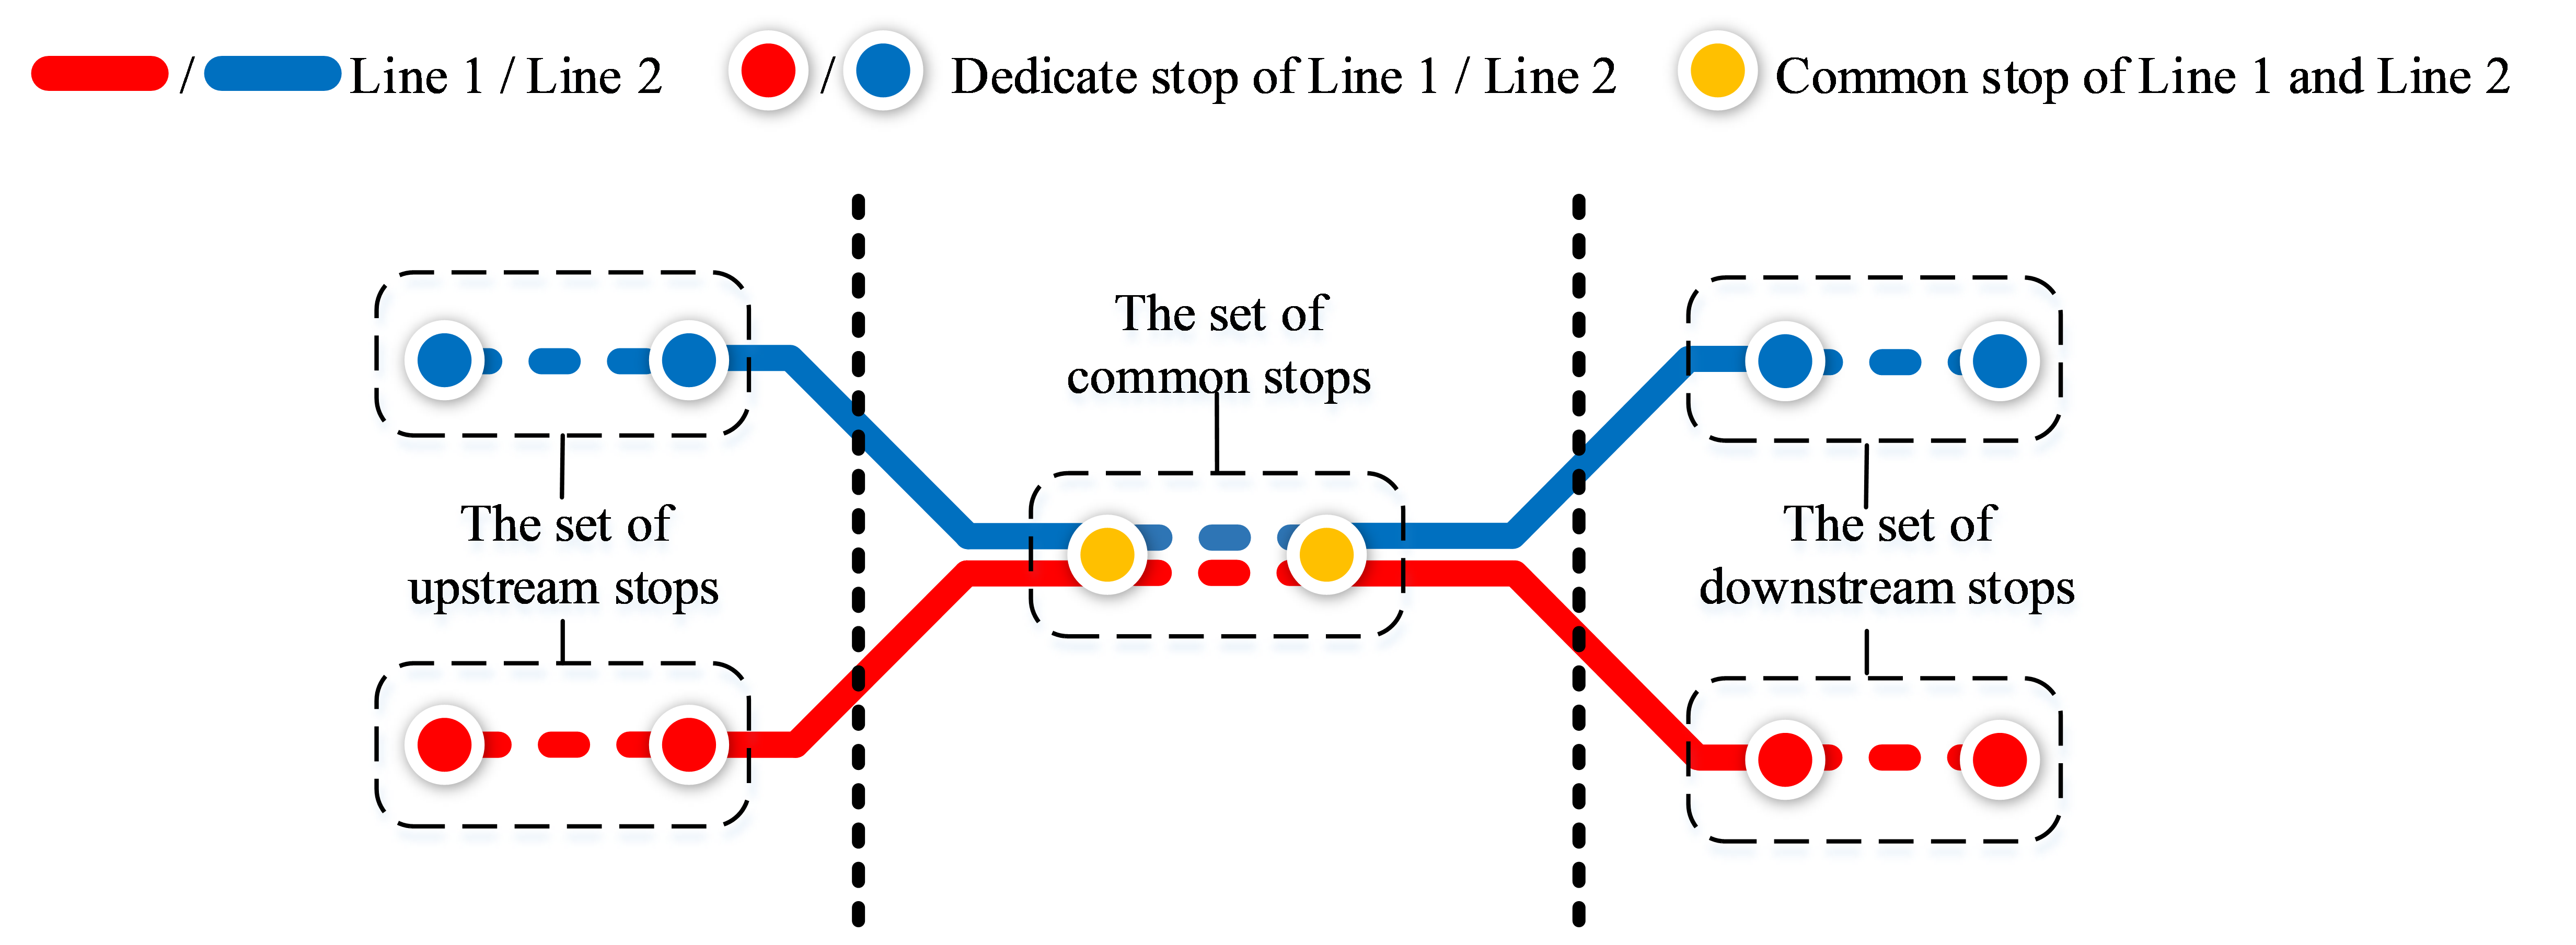
\includegraphics[width=0.9\linewidth]{CASPT2021paper_fig/Fig1.png} 
  \caption{Two bus lines corridor with some common line stops} 
  \label{fig:Fig1} 
\end{figure}

It is necessary to acknowledge that the routing behavior of Type \ref{item:common}) passengers was investigated 
in \textrm{Schmöcker et al. (2016)} by a distributed boarding equilibrium with a premise that two buses dwelling at a stop and overtaking are possible.
In our study, we focus on the transfer behaviors of Type \ref{item:transfer}) passengers, which was not discussed in previous studies on bus bunching.

%TODO: Yu Jiang 


\subsection{Assumptions}
The following assumptions are made to facilitate model development.
\begin{enumerate}[{A}1)]
    \item\label{A: avoid transfer} Passengers avoid transfers unless necessary. 
    \item\label{A: OD} Passengers' demand information, including origin, destination and arrival rate, are given.
    \item\label{A: constant supply and demand} Buses are operated at a constant frequency at the terminal station. 
    \item\label{A: T} Travel times on roads between two successive common stops are equal for buses of two lines.
    \item\label{A: FAFD} A stop has only one platform for passengers to board/alight and buses are not allowed to overtake each other or skip a stop. 
    \item\label{A: dwell time} The time required for boarding/alighting is estimated to be proportional of the number of boarding/alighting passengers.
    % It is necessary to acknowledge that
    % the routing behavior of Type \ref{item:common}) passengers is discussed
    % by \textrm{Schmöcker et al. (2016)} with a distributed boarding equilibrium 
    % assumed two buses dwelling at a stop and overtaking are possible.
    % This assumption corresponds to the one-platform stop design 
    % and no-overtaking operational strategy in their work. 
    % Considering bus capacity constraint but neglect the addition time to open and close doors,
    % the dwell time could be zero at a stop with no boarding or alighting demand.
    % Find more literature    
\end{enumerate}

According to A\ref{A: avoid transfer}),Type \ref{item:transfer}) passengers only transfer once and other passengers do not make any transfer once they board buses that lead to their destinations.
With A\ref{A: FAFD}), a bus arriving at a stop occupied by another bus will queue outside the platform until the preceding bus departs.
Therefore, buses follow the first-arrive-first-depart (FAFD) rule, which is usual for two lines sharing one platform at a common stop in real life without skipping or overtaking schemes.
A\ref{A: T}) is made so as to focus on how passengers' behaviors disturb the bus travel time via affecting bus dwell times \citep{2014Muoz,2015Carlos,2016Sun}(Muñoz et al., 2013; Hernández et al., 2015; Schmöcker et al., 2016). This assumption eliminates the impacts from traffic condition. Nevertheless, it is reasonable if the stops are connected by dedicated bus lanes and different bus lines operated with the same type of vehicles. 
A\ref{A: constant supply and demand}) is realistic for a high-frequency bus route or in peak hours 
and is commonly adopted in existing literature \citep{2016Sanchez,2016Sun,2017Wu}.
A\ref{A: dwell time} can be found in \citep{2017Wu,2019Li,2020Wang}. For a bus with two doors for boarding and alighting respectively, bus dwell time without control schemes equals the maximum value of passengers' boarding and alighting times.

% With A\ref{A: FAFD}) and A\ref{A: T}), it is reasonable for Type \ref{item:common}) passengers at common stops to prioritize the first bus among their candidate lines.
% As we mentioned before, bus bunching is prevalent in routes with high bus service frequency and passenger demands.

 % \paragraph{Paragraph headings} Use paragraph headings as needed.
% \begin{equation}
% a^2+b^2=c^2
% \end{equation}

% For two-column wide figures use
% \begin{figure*}
% \begin{center}
% % Use the relevant command to insert your figure file.
% % For example, with the graphicx package use
%   \includegraphics[width=0.8\textwidth]{Example.pdf}
% % figure caption is below the figure
% \caption{Please write your figure caption here}
% \label{fig:2}       % Give a unique label
% \end{center}
% \end{figure*}
%
% For tables use
% \begin{table}[H]
% % table caption is above the table
% \caption{Please write your table caption here}
% \label{tab:1}       % Give a unique label
% % For LaTeX tables use
% \begin{tabular}{lll}
% \hline\noalign{\smallskip}
% first & second & third  \\
% \noalign{\smallskip}\hline\noalign{\smallskip}
% number & number & number \\
% number & number & number \\
% \noalign{\smallskip}\hline
% \end{tabular}
% \end{table}

\subsection{Notations}
The following key notations are used throughout this paper.\newpage
\begin{table}[H]

  \caption{\textup{Notations}}
  \label{tab:Notations}
  \begin{tabular}{p{1.5cm}p{8.5cm}}
      \hline
      \multicolumn{2}{l}{Indices and sets }                                                                                 \\ \hline
      $r,r'$                          & Indices of bus lines                                                                \\ 
      $\mathcal{S}^{r}$               & The set of bus stops traversed by line $r$                                          \\ 
      $\mathcal{N}_{up}^{r}$          & The set of upstream stops with respect to the common stops of line $r$              \\ 
      $\mathcal{N}_{down}^{r}$        & The set of downstream stops with respect to the common stops of line $r$            \\ 
      $\mathcal{N}_{com}^{r,r'}$      & The set of common stops of line $r$ and $r'$                                        \\ 
      $\mathcal{M}^{r}$               & The set of buses of line $r$                                                        \\ 
      $m_{k}^{r}$                     & The $k^{th}$ bus of line $r$, and $k=1,2,...,\left|\mathcal{M}^{r}\right|$          \\ 
      $n_{k}^{r}$                     & The $k^{th}$ stop of line $r$, and $k=1,2,...,\left|\mathcal{S}^{r}\right|$         \\ 
      $n_{k}$                         & The $k^{th}$ stop in the common corridor, and $k=1,2,...,\left|\mathcal{N}_{com}^{r,r'}\right|$\\ 
      $m$                             & The index of the bus, $m=m_{1}^{r},...,m_{\left|\mathcal{M}^{r}\right|}^{r},m_{1}^{r'},...,m_{\left|\mathcal{M}^{r'}\right|}^{r'}$      \\ 
      $n$                             & The index of the bus stop, $n=n_{1}^{r},...,n_{\left|\mathcal{S}^{r}\right|}^{r},n_{1}^{r'},...,n_{\left|\mathcal{S}^{r'}\right|}^{r'}$ \\ 
      $\mathcal{S}^{D}(n)$            & The set of destination stops associated with the passengers arriving at\\ & stop $n$    \\ 
      $\mathcal{M}^{S}(n)$            & The set of buses serving stop $n$                                                   \\ 
      $m^{r,r'}(m,n)$                 & The index of the last bus departing from the common stop $n$ before bus $m$         \\ 
      $n^{r}(n)$                      & The index of the subsequent bus stop after stop $n$ in line $r$                     \\ 
  \end{tabular}
  % \end{table}
  % \begin{table}[H]
    \begin{tabular}{p{1.5cm}p{7cm}p{1.1cm}}
      \hline
      \multicolumn{2}{l}{Parameters}                                                                                                   & Unit\\ \hline
      $\Lambda_{n}$                   & The arrival rate of passengers at stop $n$                                                     & pas/min \\ 
      $\Lambda_{n}^{r}$               & The arrival rate of passengers at stop $n$ whose candidate line is line $r$                    & pas/min \\ 
      $\Lambda_{n}^{r,r'}$            & The arrival rate of passengers at stop $n$ whose candidate lines are line $r$ and line $r'$    & pas/min \\ 
      $\lambda_{i,j}$                 & The arrival rate of passengers whose origin and destination are stops $i$ and $j$ respectively & pas/min \\ 
      $H^{r}$                         & The scheduled bus departure headway of line $r$                                                & min     \\ 
      $cap_{m}$                       & The vehicle capacity of bus $m$                                                                & pas     \\ 
      $\beta$                         & The average boarding rate of passengers                                                        & pas/min \\ 
      $\alpha$                        & The average alighting rate of passengers                                                       & pas/min \\ 
      $T_{m,n}$                       & The travel time for bus $m$ between stop $n$ and its subsequent stop                           & min     \\\hline
  \end{tabular}
  \end{table}\newpage
\begin{table}[H]
  \begin{tabular}{p{1.5cm}p{7cm}p{1.1cm}}
    \hline
    Variables                       &                                                                                                                    & Unit\\ \hline
    $a_{m,n}$                       & The arrival time of bus $m$ at stop $n$                                                                            & min \\ 
    $W_{m,n}$                       & The dwell time of bus $m$ at stop $n$                                                                              & min \\ 
    $d_{m,n}$                       & The departure time of bus $m$ from stop $n$                                                                        & min \\ 
    $C_{m,n}$                       & The available capacity of bus $m$ at stop $n$                                                                      & pas \\ 
    $A_{m,n}$                       & The number of alighting passengers of bus $m$ at stop $n$                                                          & pas \\ 
    $\bar{B}_{m,n}$                 & The number of boarding passengers of bus $m$ at stop $n$                                                           & pas \\ 
    $B_{m,n}$                       & The number of passengers who want to board bus $m$ at stop $n$                                                     & pas \\ 
    $p_{m,n,j}$                     & The number of onboard passengers whose destination is stop $j$                                                     & pas \\ 
                                    & when bus $m$ arrives at stop $n$         \\ 
    $P_{m,n}$                       & The total number of onboard passengers when bus $m$ arrives at stop $n$                                            & pas \\ 
    $L_{m,n}$                       & The total number of leftover passengers at stop $n$ when bus $m$ departs                                           & pas \\ 
    $L_{m,n}^{r}$                   & The number of leftover passengers at stop $n$ when bus $m$                                                         & pas \\ 
                                    & departs whose candidate lines is line $r$ \\ 
    $L_{m,n}^{r,r'}$                & The number of leftover passengers at stop $n$ when bus $m$                                                         & pas \\
                                    & departs whose candidate lines are line $r$ and line $r'$ \\ 
    $l_{m,n,j}$                     & The number of leftover passengers whose destination is stop $j$                                                    & min \\
                                    & when bus $m$ departs from stop $n$.\\ 
    $h_{m,n}^{r,r'}$                & The headway between bus $m$ and its preceding bus of either line $r$ or line $r'$ at stop                          & min \\ 
    $h_{m,n}^{r}$                   & The headway between bus $m$ and $m-1$ of line $r$ at stop $n$                                                      & min \\ 
    $\bar{\rho}_{m,n}$              & The proportion of alighting transfer passengers among all                                                          &     \\
                                    & transfer passengers onboard when bus $m$ dwells at stop $n$. \\ 
    $\alpha_{n}^{m,n}$              & The proportion of transfer passengers choosing stop $n$ as a                                                       &     \\
                                    & transfer stop among all transfer passengers from bus $m'$ \\
                                    & to bus $m$.\\
    $\omega^{m',m}$                  & The minimum transfer time from bus $m'$ to the other line                                                          & min \\  
    $\omega_{n}^{m'}$               & The transfer time from bus $m'$ to the other line via common stop $n$                                              & min \\ 
    $\omega_{n}^{m'}$               & The transfer time from bus $m'$ to bus $m$ common stop $n$                                                         & min \\ \hline

\end{tabular}
\end{table}

\section{Bus motion model}\label{Bus movement}
In general, bus movement can be decomposed into two parts, one is running on the road and the other is dwelling at stops. Correspondingly, bus travel time includes running time and dwelling time.
Based on assumption A\ref{A: T}, the main source that affects bus travel time considered in this study is the dwell time, which is determined by the number of boarding and alighting passengers. 
Therefore, this subsection starts with formulating the number of boarding and alighting passengers considering routing behavior and capacity constraints. Afterwards, the bus dwell time is computed and the algorithm for finding bus trajectories is depicted.

\subsection{Boarding demand}\label{B}
First, we identify the boarding demands of passengers at common stops.
Based on A\ref{A: constant supply and demand}) and A\ref{A: OD}), 
the total arrival rate at stop $n$, denoted as $\Lambda_{n}$ (pas/min), 
is divided into $\lambda_{n,j}$ 
according to their destinations $j\in \mathcal{S}^{D}(n)$.
$\mathcal{S}^{D}\left( n \right)$ denotes the set of all destinations of arriving passengers 
at stop $n$ can be accessed,
and then $\Lambda_{n}$ can be obtained by:
\begin{equation}
    \label{equ:sumLambda}
    \Lambda_{n} = \sum_{j \in \mathcal{S}^{D}\left( n \right)} \lambda_{n,j} 
\end{equation}

For example, for the $i^{th}$ upstream stop of line 1
(i.e. $n=n^{1}_{i} \in \mathcal{N}_{up}^{1}$) in \textup{Fig. 1}, 
its set of destination stops is 
$\mathcal{S}^{D}\left( n^{1}_{i} \right) = 
\left\{ n^{1}_{k}|n^{1}_{k} \in \mathcal{S}^{1},k > i \right\}
\cup \mathcal{N}_{down}^{2}$ , 
which indicates that the arriving passengers contain two cases:
\begin{enumerate}[1)]
    \item A passenger boards at the upstream stop and alight 
    at one of the subsequent stops of the same line 
    (i.e. $\left\{ n^{1}_{k}|n^{1}_{k} \in \mathcal{S}^{1},k > i \right\}$).
    \item A passenger boards at the upstream stop and alight at one of the downstream stops of the other line 
    (i.e. $\mathcal{N}_{down}^{2}$ ), 
    so he/she needs to choose a common stop to make a transfer.
\end{enumerate}

More generally, the arrival passengers at a common stop served by multi bus lines could be grouped according to their candidate lines.
At common stop $n$ traversed by line $r$ and line $r'$ (i.e. $n\in \mathcal{N}_{com}^{r,r'}$ in Fig.\ref{fig:Fig1}), 
the total arrival rate of passengers $\Lambda_{n}$ is divided into three parts:
\begin{equation}
    \label{equ:catlambda}
    \Lambda_{n} = \Lambda_{n}^{r} + \Lambda_{n}^{r'} + \Lambda_{n}^{r,r'}
\end{equation}

\begin{enumerate}[1)]
  \item $\Lambda_{n}^{r}$ denotes the total arrival rate of passengers 
  who only consider boarding a bus belonging to line $r$ at stop $n$ and is calculated by:
  \begin{equation}
      \Lambda_{n}^{r} = \sum_{j \in \mathcal{S}^{D}(n)\backslash\mathcal{S}^{r'}} \lambda_{n,j}
  \end{equation}
  \item $\Lambda_{n}^{r'}$ denotes the total arrival rate of passengers 
  who only consider boarding a bus belonging to line $r'$ at stop $n$ and is calculated by:
  \begin{equation}
      \Lambda_{n}^{r'} = \sum_{j \in \mathcal{S}^{D}(n)\backslash\mathcal{S}^{r}} \lambda_{n,j}
  \end{equation}
  \item $\Lambda_{n}^{r,r'}$ denotes the total arrival rate of passengers that consider boarding a bus belonging to either line $r$ or line $r'$ at stop $n$,
  since their destination is one of the common stops, and it is calculated by:
  \begin{equation}
      \Lambda_{n}^{r,r'} = \sum_{j \in \mathcal{S}^{D}\left(n\right) \cap \mathcal{N}_{com}^{r,r'}} \lambda_{n,j}
  \end{equation}
\end{enumerate}

The boarding demand of a specific bus contains all passengers whose candidate sets include this bus line.
At common stop $n$ traversed by line $r$ and line $r'$, 
the boarding demands $B_{m,n}$ of the bus $m$ of line $r$ (i.e. $m=m^{r}_{k}$, $k=1,2,3,...,\left|\mathcal{M}^{r}\right|$) 
are composed of $B_{m,n}^{r}$ and $B_{m,n}^{r,r'}$ defined as follows.
\begin{enumerate}[1)]
    \item $B_{m,n}^{r}$ denotes the number of passengers whose destinations are dedicated stops of line $r$. 
    \item $B_{m,n}^{r,r'}$ denotes the number of passengers whose destination are common stops traversed by line $r$ and line $r'$. 
\end{enumerate}

The number of boarding passengers is calculated by the sum of the two types of passengers:
\begin{equation}
    B_{m,n}=B_{m,n}^{r}+B_{m,n}^{r,r'}
\end{equation}

Due to the capacity constraint, 
each type of passenger demand is composed of new arriving passengers 
and leftover passengers who already arrived before the preceding bus departing.
Denote $m^{r,r'}\left(m,n\right)$ as the index of the preceding bus departing from stop $n$ before bus $m$.
Mathematically, it is expressed by
\begin{equation}
    m^{r,r'}\left(m,n\right)=\arg \max_{m'} \left\{d_{m',n} | d_{m',n} < d_{m,n},m'\in\mathcal{M}^{r} \cup \mathcal{M}^{r'}\right\}
\end{equation}
where $d_{m,n}$, $d_{m',n}$ denote the departure time of bus $m$ and bus $m'$ from stop $n$, respectively. 

The headway between buses $m$ and $m^{r,r'}\left(m,n\right)$ at stop $n$ is obtained by:
\begin{equation}
    \label{equ:headway}
    h_{m,n}^{r,r'}=d_{m,n}-d_{m^{r,r'}\left(m,n\right),n}
\end{equation}

Thus, $B_{m,n}^{r}$, $B_{m,n}^{r,r'}$ and $B_{m,n}$ can be calculated by:
\begin{equation}\label{equ:B^r}
    B_{m,n}^{r} = \Lambda_{n}^{r} \cdot h_{m,n}^{r,r'} + L_{m^{r,r'}\left(m,n\right),n}^{r} + L_{m^{r,r'}\left(m,n\right),n}^{r}
\end{equation}
\begin{equation}\label{equ:B^rr'}
    B_{m,n}^{r,r'} = \Lambda_{n}^{r,r'} \cdot h_{m,n}^{r,r'} + L_{m^{r,r'}\left(m,n\right),n}^{r} + L_{m^{r,r'}\left(m,n\right),n}^{r,r'}
\end{equation}
\begin{equation}
    \label{equ:totalB}
    B_{m,n} = \left(\Lambda_{n}^{r} + \Lambda_{n}^{r,r'}\right) \cdot h_{m,n}^{r,r'} + L_{m^{r,r'}\left(m,n\right),n}^{r} + L_{m^{r,r'}\left(m,n\right),n}^{r,r'}
\end{equation}
where $L_{m^{r,r'}\left(m,n\right),n}^{r}$ and $L_{m^{r,r'}\left(m,n\right),n}^{r,r'}$ 
denote the numbers of leftover passengers who arrived before the last bus depart and their computations are introduced in \ref{P and L}.

The equations for common stops (i.e. Eq.(\ref{equ:catlambda})-(\ref{equ:totalB})) are valid for dedicated stops.
For example, for a dedicated stop $n$ which only served by a single line $r$,
the formulations are degenerated by $\Lambda_{n}^{r'},\Lambda_{n}^{r,r'}=0$ 
and for the  $k^{th}$ bus of line $r$ (i.e. $m=m^{r}_{k}$, $k=2,3,...,\left|\mathcal{M}^{r}\right|)$, $m^{r,r'}\left(m,n\right)=m^{r}_{k-1}=m-1$.
Therefore, Eq.(\ref{equ:catlambda}),Eq.(\ref{equ:headway}) and Eq.(\ref{equ:totalB}) are degenerated into 
\begin{equation}
    \Lambda_{n} = \sum_{j \in \mathcal{S}^{D}\left(n\right)} \lambda_{n,j} = \Lambda_{n}^{r},
\end{equation}

\begin{equation}
    h_{m,n}^{r}=d_{m,n}-d_{m-1,n}
\end{equation}
and
\begin{equation}
    \label{equ:singleB}
    B_{m,n} = B_{m,n}^{r} = \Lambda_{n}^{r} \cdot h_{m,n}^{r} + L_{m-1,n}^{r} 
\end{equation}

\subsection{Number of boarding passengers under capacity constraint}\label{barB}
The actual number of boarding passengers is constrained by the bus available capacity.
At common stop $n$, the actual number of boarding passengers of bus $m$, 
denoted as $\overline{B}_{m,n}$, is refined by:
\begin{equation}
    \label{equ:barB}
    \overline{B}_{m,n} = \min \left\{C_{m,n},B_{m,n}\right\}
\end{equation}
where $C_{m,n}$ denote the available capacity when bus $m$ arrives at stop $n$.

Therefore, the formulations of numbers of alighting and onboard passengers are necessary as $C_{m,n}$ is calculated by: 
\begin{equation}
    \label{equ:C}
    C_{m,n} = cap_{m} - P_{m,n} + A_{m,n}
\end{equation}
where $cap_{m}$ denotes the designed capacity of bus $m$, 
$P_{m,n}$ denotes the number of onboard passengers of bus $m$ when it arrives at stop $n$, 
and $A_{m,n}$ denotes the number of alighting passengers of bus $m$ at stop $n$.
Alighting passengers of bus $m$ at common stop $n$ include the passengers 
whose destination is stop $n$ and parts of transfer passengers who choose stop $n$ as their interchange stop 
and $A_{m,n}$ can be calculated by:
\begin{equation}
    \label{equ:A}
    A_{m,n} = p_{m,n,n} + \overline{\rho}_{m,n} \cdot \sum_{j \in \mathcal{S}^{D}(n)\backslash\mathcal{S}^{r}}  p_{m,n,j}
\end{equation}

In \textup{Eq.(\ref{equ:A})}, $p_{m,n,j}$ denotes the number of onboard passengers whose destination is stop $j$  
when bus $m$ is arriving at the stop $n$. 
$\overline{\rho}_{m,n}$ denotes the proportion of passengers transferring at stop $n$ 
among all Type I) passengers on bus $m$ and is identified by a so-called
transfer-based equilibrium introduced in \ref{equilibrium}.

\subsection{Numbers of leftover and onboard passengers}\label{P and L}
Formulations above (i.e. Eq.(\ref{equ:totalB}), Eq.(\ref{equ:singleB}) and Eq.(\ref{equ:C})) indicate that 
it is necessary to identify the numbers of leftover passengers at stops as well as onboard passengers when buses depart.
As the subsequent stop of stop $n$ traversed by line $r$ is denoted as $n^{r}\left(n\right)$,
the numbers of leftover and onboard passengers
whose destination is stop $j$ 
when bus $m$ departs from stop $n$ (or arrives at $n^{r}\left(n\right)$)
are denoted as $l_{m,n,j}$ and $p_{m,n^{r}(n),j}$, respectively. 
And they can be obtained by:
\begin{equation}
  \label{equ:l}
  l_{m,n,j} = 
  \begin{cases} 
      \left(\lambda_{n,j}\cdot h_{m,n}^{r,r'}+l_{m^{r,r'}(m,n),n,j} \right)\cdot \left(1-\frac{\overline{B}_{m,n}}{B_{m,n}}\right)&\text{if } j \in \mathcal{S}^{D}(n)\cap\mathcal{S}^{r}\\
      \lambda_{n,j}\cdot h_{m,n}^{r,r'}+l_{m^{r,r'}(m,n),n,j}+\overline{\rho}_{m,n}\cdot p_{m,n,j}&\text{if } j \in \mathcal{S}^{D}(n)\backslash\mathcal{S}^{r}
  \end{cases}    
\end{equation}
and
\begin{equation}
    \label{equ:p}
    p_{m,n^{r}(n),j} = 
    \begin{cases} 
        p_{m,n,j} + \left(\lambda_{n,j}\cdot h_{m,n}^{r,r'}+l_{m^{r,r'}\left(m,n\right),n,j}\right)\cdot \frac{\overline{B}_{m,n}}{B_{m,n}}&\text{if } j \in \mathcal{S}^{D}(n)\cap\mathcal{S}^{r}\\
        \left(1-\overline{\rho}_{m,n}\right)\cdot p_{m,n,j}&\text{if } j \in \mathcal{S}^{D}(n)\backslash\mathcal{S}^{r}
    \end{cases}    
\end{equation}
% where $\left(1-\overline{\rho}_{m,n}\right)\cdot p_{m,n,j}$ is corresponding to the passengers 
% whose destinations belong to the other line but have not made the transfer yet. 

There are two points need to acknowledge in \textup{Eq.(\ref{equ:l}) and Eq.(\ref{equ:p})}:
\begin{enumerate}[1)]
    \item The proportion of each kind of passengers in the boarding passengers is assumed to
    be equal to the proportion of this kind of passengers in the accumulated queue passengers in boarding progress. 
    In other words, the probabilities of boarding successfully of all passengers involved in a boarding process 
    is equal to the ratio of the number of boarding passengers to the boarding demand (i.e. $\frac{\overline{B}_{m,n}}{B_{m,n}}$ in Eq.(\ref{equ:l}) and Eq.(\ref{equ:p})).
    \item  The concept of \textit{leftover passengers} is different 
    from that in single-line models where it only refers to passengers failed to board an earlier bus 
    due to the capacity constraint.
    For example, the leftover passengers at a common stop when bus $m$ of line $r$ departs include all passengers 
    whose candidate set of lines doesn't contain line $r$.
\end{enumerate}

Then, the total numbers of leftover and onboard passengers can be calculated by:
\begin{equation}
    \label{equ:P}
    P_{m,n^{r}(n)} = \sum_{j\in \mathcal{S}^{D}(n)} p_{m,n^{r}(n),j}
\end{equation}
and
\begin{equation}
    L_{m,n} = \sum_{j\in\mathcal{S}^{D}(n)} l_{m,n,j}
\end{equation}

To facilitate the computations of boarding demands 
(i.e. \textup{Eq.(\ref{equ:B^r}), Eq.(\ref{equ:B^rr'}) and Eq.(\ref{equ:totalB})}) in \ref{B}, 
the numbers of leftover passengers divided according to their candidate lines are needed:
\begin{equation}
    \label{equ:Lr}
    L_{m,n}^{r} = \sum_{j\in\mathcal{S}^{D}(n)\backslash\mathcal{S}^{r'}} l_{m,n,j}
\end{equation}
\begin{equation}
    L_{m,n}^{r'} = \sum_{j\in\mathcal{S}^{D}(n)\backslash\mathcal{S}^{r}} l_{m,n,j}
\end{equation}
\begin{equation}
    L_{m,n}^{r,r'} = \sum_{j\in\mathcal{S}^{D}(n)\cap \mathcal{S}^{r}\cap \mathcal{S}^{r'}} l_{m,n,j}
\end{equation}

% \subsection{Bus dwell time constrained by bus capacity and passenger alighting time}
\subsection{Bus dwell time}
Inspired by existing work about single-line model considering bus capcaity constant (i.e. Wu et al., 2017), 
we derive bus dwell time by formulating the queue clearance time of passenger boarding demand 
and constrain it by available capacity on bus and passenger alighting time.
% \subsubsection{Boarding queue clearance time}
Based on the assumption of constant passengers' arrivals and boarding rates, 
the boarding queue clearance time can be obtained by 
$\frac{\text{The initial queue length}}{\text{The queue clearance rate}}$. 
Particularly, at a common stop $n$ traversed by line $r$ and line $r'$, 
% the initial length of the boarding queue is 
% $[\left(a_{m,n}-d_{m^{r,r'}(m,n),n}\right)\cdot \left(\Lambda_{n}^{r}+\Lambda_{n}^{r,r'}\right)+L_{m^{r,r'}(m,n),n}^{r}+L_{m^{r,r'}(m,n),n}^{r,r'}]$
% and the clearance rate is $[\beta-\left(\Lambda_{n}^{r}+\Lambda_{n}^{r,r'}\right)]$. 
% Therefore, 
the boarding queue clearance time for bus $m$ denoted by $W_{m,n}^{B}$ can be obtained by:
\begin{equation}
    W_{m,n}^{B} = \frac{\left(a_{m,n}-d_{m^{r,r'}(m,n),n}\right)\cdot \left(\Lambda_{n}^{r}+\Lambda_{n}^{r,r'}\right)
    +L_{m^{r,r'}(m,n),n}^{r}+L_{m^{r,r'}(m,n),n}^{r,r'}}
    {\beta-\left(\Lambda_{n}^{r}+\Lambda_{n}^{r,r'}\right)}
\end{equation}
where $a_{m,n}$ denotes the arrival time of bus $m$ at stop $n$ 
and $\beta$ denotes the average boarding rate of passengers. 
In this work, it is assumed that the boarding rate is much larger than 
passenger arrival rates (i.e. $\beta \gg \Lambda_{n}$ for all stop $n$). 

For the simplicity of formulas, 
we introduce the bus service empty period referring to the period during which there is no bus dwelling at the stop. 
For example, when the bus service empty period at stop $n$ ended up with the arrival of $m$, 
the length of the period, denoted by $I_{m,n}^{r,r'}$, is obtained by:
\begin{equation}
    I_{m,n}^{r,r'} = a_{m,n} - d_{m^{r,r'}(m,n),n}
\end{equation}

Then, the expression of boarding queue clearance time can be expressed as:
\begin{equation}
    \label{equ:WB}
    W_{m,n}^{B} = \frac{I_{m,n}^{r,r'}\cdot \left(\Lambda_{n}^{r}+\Lambda_{n}^{r,r'}\right)
    +L_{m^{r,r'}(m,n),n}^{r}+L_{m^{r,r'}(m,n),n}^{r,r'}}
    {\beta-\left(\Lambda_{n}^{r}+\Lambda_{n}^{r,r'}\right)}
\end{equation}

The passenger alighting time of bus $m$ of line $r$ at stop $n$, denoted as $W_{m,n}^{A}$, can be calculated by:
\begin{equation}
    \label{equ:WA}
    W_{m,n}^{A} = \frac{A_{m,n}}{\alpha} %\text{ for } m \in \mathcal{M}^{1}\cup \mathcal{M}^{2};n\in \mathcal{S}^{1}\cup\mathcal{S}^{2}
\end{equation}
where $\alpha$ denotes the average alighting rate of passengers. 

As a result, the actual dwell time of bus $m$ at stop $n$, denoted as $W_{m,n}$,
is the maximum value between the boarding and alighting time:
\begin{equation}
    \label{equ:W}
    W_{m,n} = \max \left\{W_{m,n}^{A},\min \left\{W_{m,n}^{B},\frac{C_{m,n}}{\beta}\right\}\right\}
    \text{ for } m \in \mathcal{M}^{1}\cup \mathcal{M}^{2};n\in \mathcal{S}^{1}\cup\mathcal{S}^{2}
\end{equation}

\subsection{Algorithm for bus trajectories}
Before conducting the calculations for bus dwell times and bus trajectories,
some initialization is needed to start the algorithm.

\begin{enumerate}[1)]
    \item Initialize the bus arrival times at the first stop of each line
\end{enumerate}

We denote the arrival time at the first bus stop of the first bus of line $r$ as $t^{r}$ (for $r=1,2$), 
based on the assumption about constant bus depart frequency in A\ref{A: constant supply and demand}), 
the arrival times of all buses of line $r$ at the first stop can be determined by:
\begin{equation}
    a_{m^{r}_{k},n^{r}_{1}} = t^{r} + H^{r} \cdot \left(k-1\right) \text{ for } k=1,2,...,\left| \mathcal{M}^{r} \right|
\end{equation}
where $H^{r}$ denotes the departure headway of line $r$. 
\begin{enumerate}[2)]
    \item Initialize dwell times of the first bus of each line at all stops served by it
\end{enumerate}

As the first bus of each line ($m=m^{r}_{1},\text{ for }r=1,2$) has no preceding bus, we presuppose:
\begin{equation}
    I_{m,n}^{r} = H^{r}, \text{for } m=m^{r}_{1};n=n^{r}_{k};k=1,2,...,\left|\mathcal{S}^{r}\right|;r=1,2
\end{equation}
and
\begin{equation}
    I_{m,n}^{r,r'} = \left(\frac{1}{H^{r}}+\frac{1}{H^{r'}}\right)^{-1}, \text{for } m=m^{r}_{1};n=n^{r}_{k};k=1,2,...,\left|\mathcal{S}^{r}\right|;r=1,2
\end{equation}
The bus dwell times of the first bus of each line at all served stops can be obtained according to Eq.(\ref{equ:WB}).

With the initialization above, the pseudocode of the algorithm for simulating bus trajectories is presented in \textbf{Algorithm \ref{algorithm}}.
\begin{algorithm}[H]
    \caption{Event-based algorithm for bus trajectories}
    \label{algorithm}
    \begin{algorithmic}
        \STATE \textbf{Input parameters}: $\alpha$,$\beta$,$\varepsilon$,$\lambda_{i,j}$,$T_{m,n}$ %for $i,j\in \mathcal{S}^{1}\cup\mathcal{S}^{2}$
        \STATE \textbf{Initialization}: $a_{m^{r}_{k},n^{r}_{1}}$ for $k=1,2,...,\left| \mathcal{M}^{r} \right|$
      \FOR{$\mathcal{N}$ $\in$ $\left\{\mathcal{N}_{up}^{1},\mathcal{N}_{up}^{2},\mathcal{N}_{com}^{1,2},\mathcal{N}_{down}^{1},\mathcal{N}_{down}^{2}\right\}$}
          \FOR{$n\in\mathcal{N}$}
%                \STATE (Case A: $n$ is a common stop; Case B: $n$ is a dedicated stop)
              \STATE Get the service bus fleet of stop $n$: $\mathcal{M}^{S}(n)$
              \FOR{$m\in\mathcal{M}^{S}(n)$ sorted by their arrival time at stop $n$}
                  \STATE Calculate the number of alighting passengers $A_{m,n}$ by Eq.(\ref{equ:A}) 
                  % for Case A and Eq.(\ref{equ:singleA}) for Case B
                  \STATE Calculate the available capacity $C_{m,n}$ by Eq.(\ref{equ:C})
                  \STATE Calculate the bus dwell time $W_{m,n}$ of bus $m$ at stop $n$ by Eq.(\ref{equ:WB}), Eq.(\ref{equ:W}) and Eq.(\ref{equ:WA})
                  \STATE Calculate the departure time of bus $m$ from stop $n$ by:
                  \begin{equation}
                      d_{m,n}=a_{m,n}+W_{m,n}
                  \end{equation}
                  \STATE Calculate the arrival time of bus $m$ at the next stop by Eq.(\ref{equ:a})
                  \STATE Calculate the number of boarding passengers $B_{m,n}$ by Eq.(\ref{equ:totalB})      
                  \STATE Calculate the number of boarding passengers $\bar{B}_{m,n}$ by Eq.(\ref{equ:barB})
                  \STATE Calculate the number of onboard passengers after boarding and alighting with Eq.(\ref{equ:p})     
                  \STATE Calculate the number of leftover passengers after boarding and alighting with Eq.(\ref{equ:l})   
                  \IF{$n$ is not the last stop of its line (i.e. $n\neq n^{r}_{\left|\mathcal{S}^{r}\right|}$)}
                      \STATE Calculate the arrival time of bus $m$ at the next stop (without loss of generality, assume bus $m$ belongs to line $r$):
                      \begin{equation}
                          \label{equ:a}
                          a_{m,n^{r}(n)}=d_{m,n}+T_{m,n}
                      \end{equation}
                  \ENDIF

              \ENDFOR
          \ENDFOR
      \ENDFOR
  \end{algorithmic}
\end{algorithm}
Moreover, there is one thing worthy noting. 
According to A\ref{A: dwell time}), the subsequent bus will queue outside the platform
if the bus arrived before the boarding process of its preceding bus finished (i.e. $a_{m,n}<d_{m^{r,r'}(m,n),n}$). 
In \textup{Eq.(\ref{equ:WB})}, we can notice that the bus boarding time could be zero
without the minimum headway, and the subsequent bus may depart together with its ahead bus in the case of no alighting demand.
Therefore, we modify the actual time arrival at platform by a minimum headway denoted as $\varepsilon>0$: 
\begin{equation}
        a_{m,n} = \max \left\{a_{m,n},d_{m^{r,r'}(m,n),n}+\varepsilon\right\} 
        \text{ for } m\in \mathcal{M}^{1}\cup\mathcal{M}^{2};
        n\in \mathcal{S}^{1}\cup\mathcal{S}^{2}
\end{equation}

\section{Passengers transfer behavior}\label{Transfer passenger routing}
\subsection{Transfer-based equilibrium}\label{equilibrium}
The computation of numbers of alighting, onboard and leftover passengers (i.e. Eq.(\ref{equ:A}), Eq.(\ref{equ:p}) and Eq.(\ref{equ:l})) requires knowing the probabilities of passengers onboard to alight and transfer to another bus at each stop, (i.e. $\bar{\rho}_{m,n}, m\in\mathcal{M}^{r}\cup\mathcal{M}^{r'},n\in\mathcal{N}_{com}^{r,r'}$), which depends on modelling passengers transfer route choice behavior among all candidate stops.  
In the light of the approach-based equilibrium formulations \textrm{(Long et al., 2013; Szeto et al., 2014; Jiang et al., 2016)}, this study proposes a transfer-based equilibrium among all Type \ref{item:transfer}) passengers on each bus to depict their transfer behavior.
To illustrate the concept, Fig.\ref{transfer choice network} is plotted.

\textcolor{red}{
    1. this study define a transfer approach as xxxx
    2. the transfer-appraoch proportion, hence, refers to xxxx, and Mathematically defined as
        also explains equation 36
    3. based on the definition of transfer appraoch, this tansfer-based equilibrium condition is given by xxx
       explain equation 37
    4. Following (liter xxxx), equation 37 can be reformulated as a NCP problem as well as Variational Inequality problem (VI)
}

We define the proportion of transfer passengers on bus $m$ 
those transfer to the other line via common stop $n_{i}$ 
are denoted as $\alpha_{n_{i}}^{m}$. 
Then, $\bar{\rho}_{m,n_{i}}$ can be written by the approach-probabilities $\alpha_{n_{i}}^{m}$ for all common stop $n_{i}\in\mathcal{N}_{com}^{r,r'}$ as:
\begin{equation}
    \bar{\rho}_{m,n_{i}} =
    \begin{cases}
        \alpha_{n_{i}}^{m}&\text{ for } i=1,\\
        \frac{\alpha_{n_{i}}^{m}}{1-\sum\limits_{k=1}^{i-1} \alpha_{n_{k}}^{m}}&\text{ for }i=2,...,\left|\mathcal{N}_{com}^{r,r'}\right|
    \end{cases} 
\end{equation}

Specifically, routing approaches of transfer passengers
from upstream stops of line $r'$ (i.e. stop $n\in\mathcal{N}_{up}^{r'}$) 
to downstream stops of line $r$ (i.e. stop $n \in \mathcal{N}_{down}^{r}$) 
via common stops (i.e. stop $n_{1},n_{2},...,n_{\left|\mathcal{N}_{com}^{r,r'}\right|}\in \mathcal{N}_{com}^{r,r'}$)
are intuitively demonstrated by the network shown in \textup{Fig.\ref{transfer choice network}}. 
\begin{figure}[H]
    \centering
    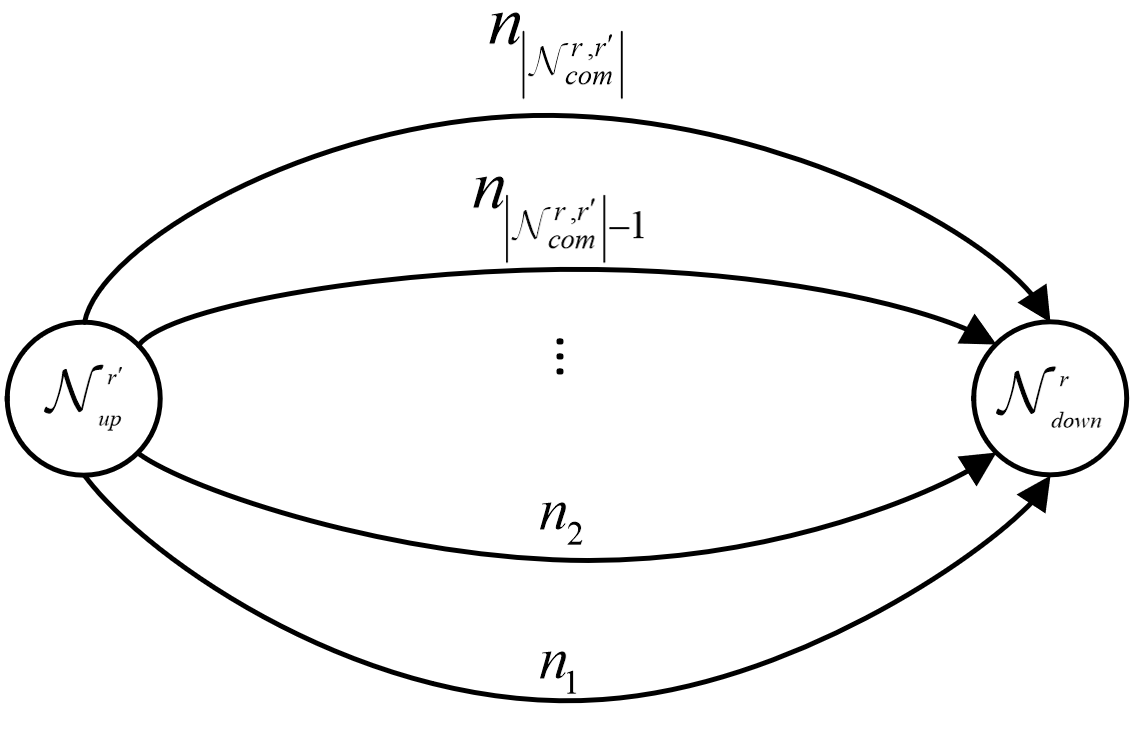
\includegraphics[width=0.5\linewidth]{CASPT2021paper_fig/transfer choice network.png}
    \caption{Transfer from from upstream stops of line $r'$ to downstream stops of line $r$ via common stops}
    \label{transfer choice network}
\end{figure}

As the transfer-based equilibrium conditions are:
\begin{equation}
    \omega_{n_{i}}^{m}
    \begin{cases}
        =\omega^{m},&\text{ if } \alpha_{n_{i}}^{m}>0\\
        \geq \omega^{m},&\text{ if } \alpha_{n_{i}}^{m}=0
    \end{cases}
    \text{ for all } n_{i} \in \mathcal{N}_{com}^{r,r'}
\end{equation}
where $\omega_{n_{i}}^{m}$ denotes the transfer cost for passengers on bus $m$ those transfer via stop $n_{i}$,
the transfer-based equilibrium constraints can be represented as follows:
\begin{equation}
    \begin{cases}
        \left(\omega_{n_{i}}^{m}-\omega^{m}\right)\cdot \alpha_{n_{i}}^{m} = 0 &\forall n_{i}\in \mathcal{N}_{com}^{r,r'}\\
        \omega_{n_{i}}^{m}-\omega^{m} \geq 0 &\forall n_{i}\in \mathcal{N}_{com}^{r,r'}\\
        0 \leq \alpha_{n_{i}}^{m} \leq 1 &\forall n_{i}\in \mathcal{N}_{com}^{r,r'}\\
        \sum\limits_{n_{i}\in \mathcal{N}_{com}^{r,r'}} \alpha_{n_{i}}^{m} = 1
    \end{cases}
\end{equation}

\textcolor{red}{the above equation can be reformulated as VI problem}

\subsection{Transfer cost function}
Without loss of generality, we assume bus $m$ is the following bus belonging line $r$ that arrives at stop $n_{i}$ 
after its preceding bus of line $r'$ which is denoted by $m^{r'}(m,n_{i})$ and can be expressed by: 
\begin{equation}
    m^{r'}\left(m,n\right)=\arg \max_{m'} \left\{d_{m',n} | d_{m',n} < d_{m,n},m'\in\mathcal{M}^{r'}\right\}
\end{equation}
% as bus $m^{r'}(m,n_{i})$ (without loss of generality and for short, we assume $m^{r'}(m,n_{i})=m'$).
According to A\ref{A: T}), bus travel times of two lines between successive common stops in the corridor are equal 
(i.e. $T_{m,n_{i}}=T_{m',n_{i}},\forall m\in\mathcal{M}^{r},m'\in\mathcal{M}^{r'},n_{i}\in \mathcal{N}_{com}^{r,r'}$).
Therefore, the arrival sequences of service buses at all common stops are as same as that at the first common stop $n_{1}$:
\begin{equation}
    m^{r'}\left(m,n_{i}\right)=m^{r'}\left(m,n_{1}\right), \forall n_{i} \in \mathcal{N}_{com}^{r,r'}
\end{equation} 

Due to the capacity constraint, part of transfer passengers on bus $m^{r'}(m,n_{i})$ may fail to board the following arrival bus $m$
as shown in Fig.\ref{fig:trans in common stop}.
\begin{figure}[H]
    \centering
    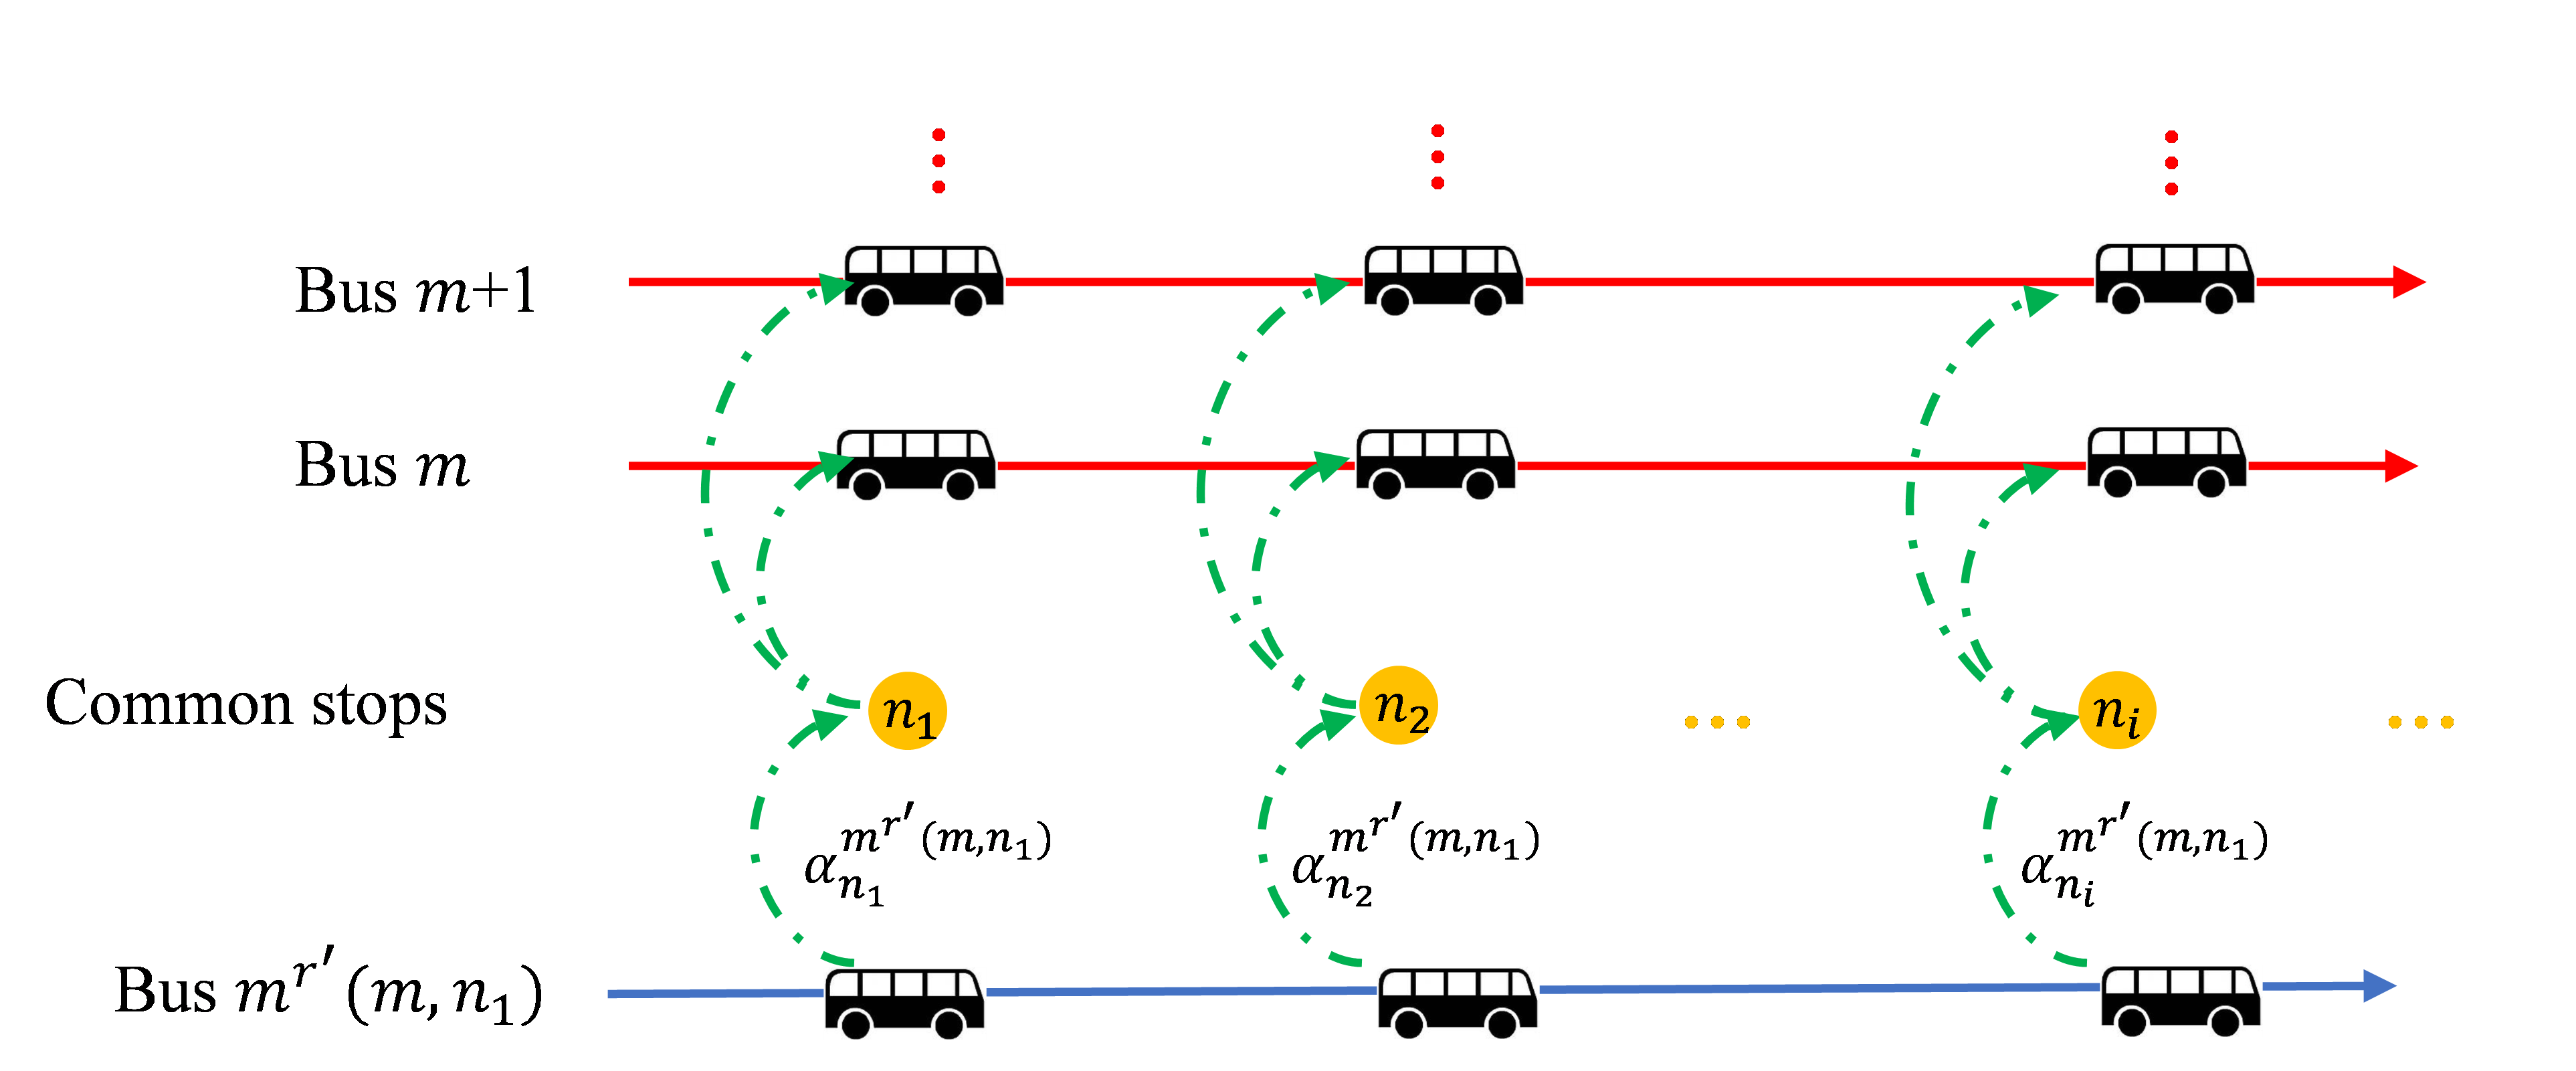
\includegraphics[width=1\linewidth]{CASPT2021paper_fig/trans in common stop.png}
    \caption{Transfer passengers from bus $m^{r'}(m,n_{i})$ to the other line via common stops}
    \label{fig:trans in common stop}
\end{figure}

The expected transfer cost function at each stop involves probabilities that transfer passengers successfully board the arrival buses.
For example, the expected cost at stop $n_{i}$ for transfer passengers from bus $m^{r'}(m,n_{i})$ is:
\begin{equation}
    \label{equ:omega}
    \begin{split}
        \omega_{n_i}^{m^{r'}(m,n_{i})} = &\frac{\overline{B}_{m,n_{i}}}{B_{m,n_{i}}}\cdot \omega_{n_i}^{m^{r'}(m,n_{i}),m} +\\
        &\left(1-\frac{\overline{B}_{m,n_{i}}}{B_{m,n_{i}}}\right)\cdot \frac{\overline{B}_{m+1,n_{i}}}{B_{m+1,n_{i}}}\cdot \omega_{n_i}^{m^{r'}(m,n_{i}),(m+1)}
        + ...        
    \end{split}
\end{equation}
where $\omega_{n_i}^{m^{r'}(m,n_{i}),m}$, $\omega_{n_i}^{m^{r'}(m,n_{i}),(m+1)}$,... 
denote the transfer time passengers from bus $m^{r'}(m,n_{i})$ to bus $m,m+1,...$, respectively.
The transfer cost between from bus $m^{r'}(m,n_{i})$ to bus $m$ is derived by the headway of the two buses:
\begin{equation}
    \begin{split}
        \omega_{n_{i}}^{m^{r'}(m,n_{i}),m}&=d_{m,n_{i}}-d_{m^{r'}(m,n_{i}),n_{i}}
    \end{split}
\end{equation}

\subsection{MSA}\label{algorithms}
To solve the VI problem and obtain the number of transfer passengers, this study adopts the method of successive average (MSA) and presented in Figure xxxxx. 
\textcolor{red}{
    1. add fig caption for the algorithm figure,
    2. although there are classic methods for solving VI.(add liter)  Nevertheless. they are not applicable in our case, since the mapping function does not have an explicit functional form, but relies on an event based simulation algorithm given in Figure. Therefore, MSA is adopted. 
}
  
\begin{algorithm}[H]
    \caption{MSA for transfer routing results}
    \label{MSA}
    \begin{algorithmic}
    \STATE \textbf{Step 0: Initialization}
    \STATE Assign the transfer passengers evenly among all common stops as an initial solution:\\
    \begin{equation}
        k=0: \alpha_{n_{i}}^{m}(1)=\frac{1}{\left|\mathcal{N}_{com}^{r,r'}\right|} \text{ for } i=1,...,\left|\mathcal{N}_{com}^{r,r'}\right|
        \text{ and } m\in \mathcal{M}^{r}\cup\mathcal{M}^{r'}
    \end{equation}
    \STATE \textbf{Step 1: $k\leftarrow k+1$ }\\
    \STATE Get all buses' transfer cost at each common stop by \textup{Eq.(\ref{equ:omega})} in the $k^{th}$ iteration: $\omega_{n_{i}}^{m'}(k)$
    \STATE \textbf{Step 2:}\\
    Get attached solution by all-or-nothing assignment: $\alpha_{n_{i}}^{m}(k)$ \\
    Calculate the new solution the average between previous solution and attached solution:\\
    \begin{equation}
        \begin{split}
            \alpha_{n_{i}}^{m}(k) \leftarrow 
            &\left(1-\frac{1}{k}\right) \cdot \alpha_{n_{i}}^{m}\left(k-1\right) + \frac{1}{k} \cdot \alpha_{n_{i}}^{m}\left( k \right)\\
            &\forall i=1,...,\left|\mathcal{N}_{com}^{r,r'}\right| \text{ and } m\in \mathcal{M}^{r}\cup\mathcal{M}^{r'}
        \end{split}
    \end{equation}
    \IF {$\alpha_{n_{i}}^{m}(k)-\alpha_{n_{i}}^{m}(k-1)>\varepsilon$}
    \STATE back to \textbf{Step 1}\\
    \ELSE 
    \STATE Stop.
    \ENDIF
    \end{algorithmic}
\end{algorithm}

% \subsection{A special realization of equilibrium assignment}
\subsection{Property}
\textcolor{red}{I think we take the special case as the property of the model}
Based on the formulations of transfer-based equilibrium and transfer cost function, a special realization of equilibrium assignment is noticeable.
According to the proposed transfer-based equilibrium, the Wardrop's first principle is fulfilled: 
for all common stops selected as interchange stops, transfer costs from line 1 to line 2 (or form line 2 to line 1) are equal.
For a common corridor with homogeneous boarding demand and served by two symmetrical bus lines (i.e. with the same service frequency and travel times on roads), the equilibrium assignment is analytical.
The explicit statement is concluded in Proposition \ref{pro:equal assignment} and a numerical verification based on MSA will be introduced in \ref{subsec: effc of trafer behaviors}. 
\begin{mypro}\label{pro:equal assignment}
    In a two-line system, equal assignment of transfer passengers among all candidate interchange stops is a special realization of equilibrium assignment when buses trajectories without disturbances are uniform in time-space diagram and all buses are not full-loaded. 
\end{mypro}
\noindent \textbf{Proof} See Appendix.$\hfill\square$ 
% \marginnote{\textcolor{red}{1}Proposition can be put in the model section}[0cm]

\section{Performance measures} \label{PM}
In this section, a set of evaluation indices are introduced to quantify the performance of bus operation affected by bus bunching and various sensitivity tests are carried to examine the performance of the model. 
\subsection{Range of evaluation}
\textcolor{red}{the title is confusing, there is no logic in the following sentence, 
also I am not quite clear the purpose of this paragraph}
As we trigger bus bunching by an initial disturbance, 
we focus on evaluating the operation of affected buses instead of the overall system.
For the example shown in Fig.\ref{fig:disturbed MSA trajectories}, Fig.\ref{fig:disturbed MSA alpha up} and Fig.\ref{fig:disturbed MSA alpha down}, 
we put a 2 min delay to the $51^{st}$ bus of line 1 (red line), 
and then, 56 bus arrivals or departures deviate from the undisturbed trajectories
% (exceeding the 1 s threshold value we set). 
as shown in Fig.\ref{fig:range}. 
\begin{figure}[H]
    \centering
    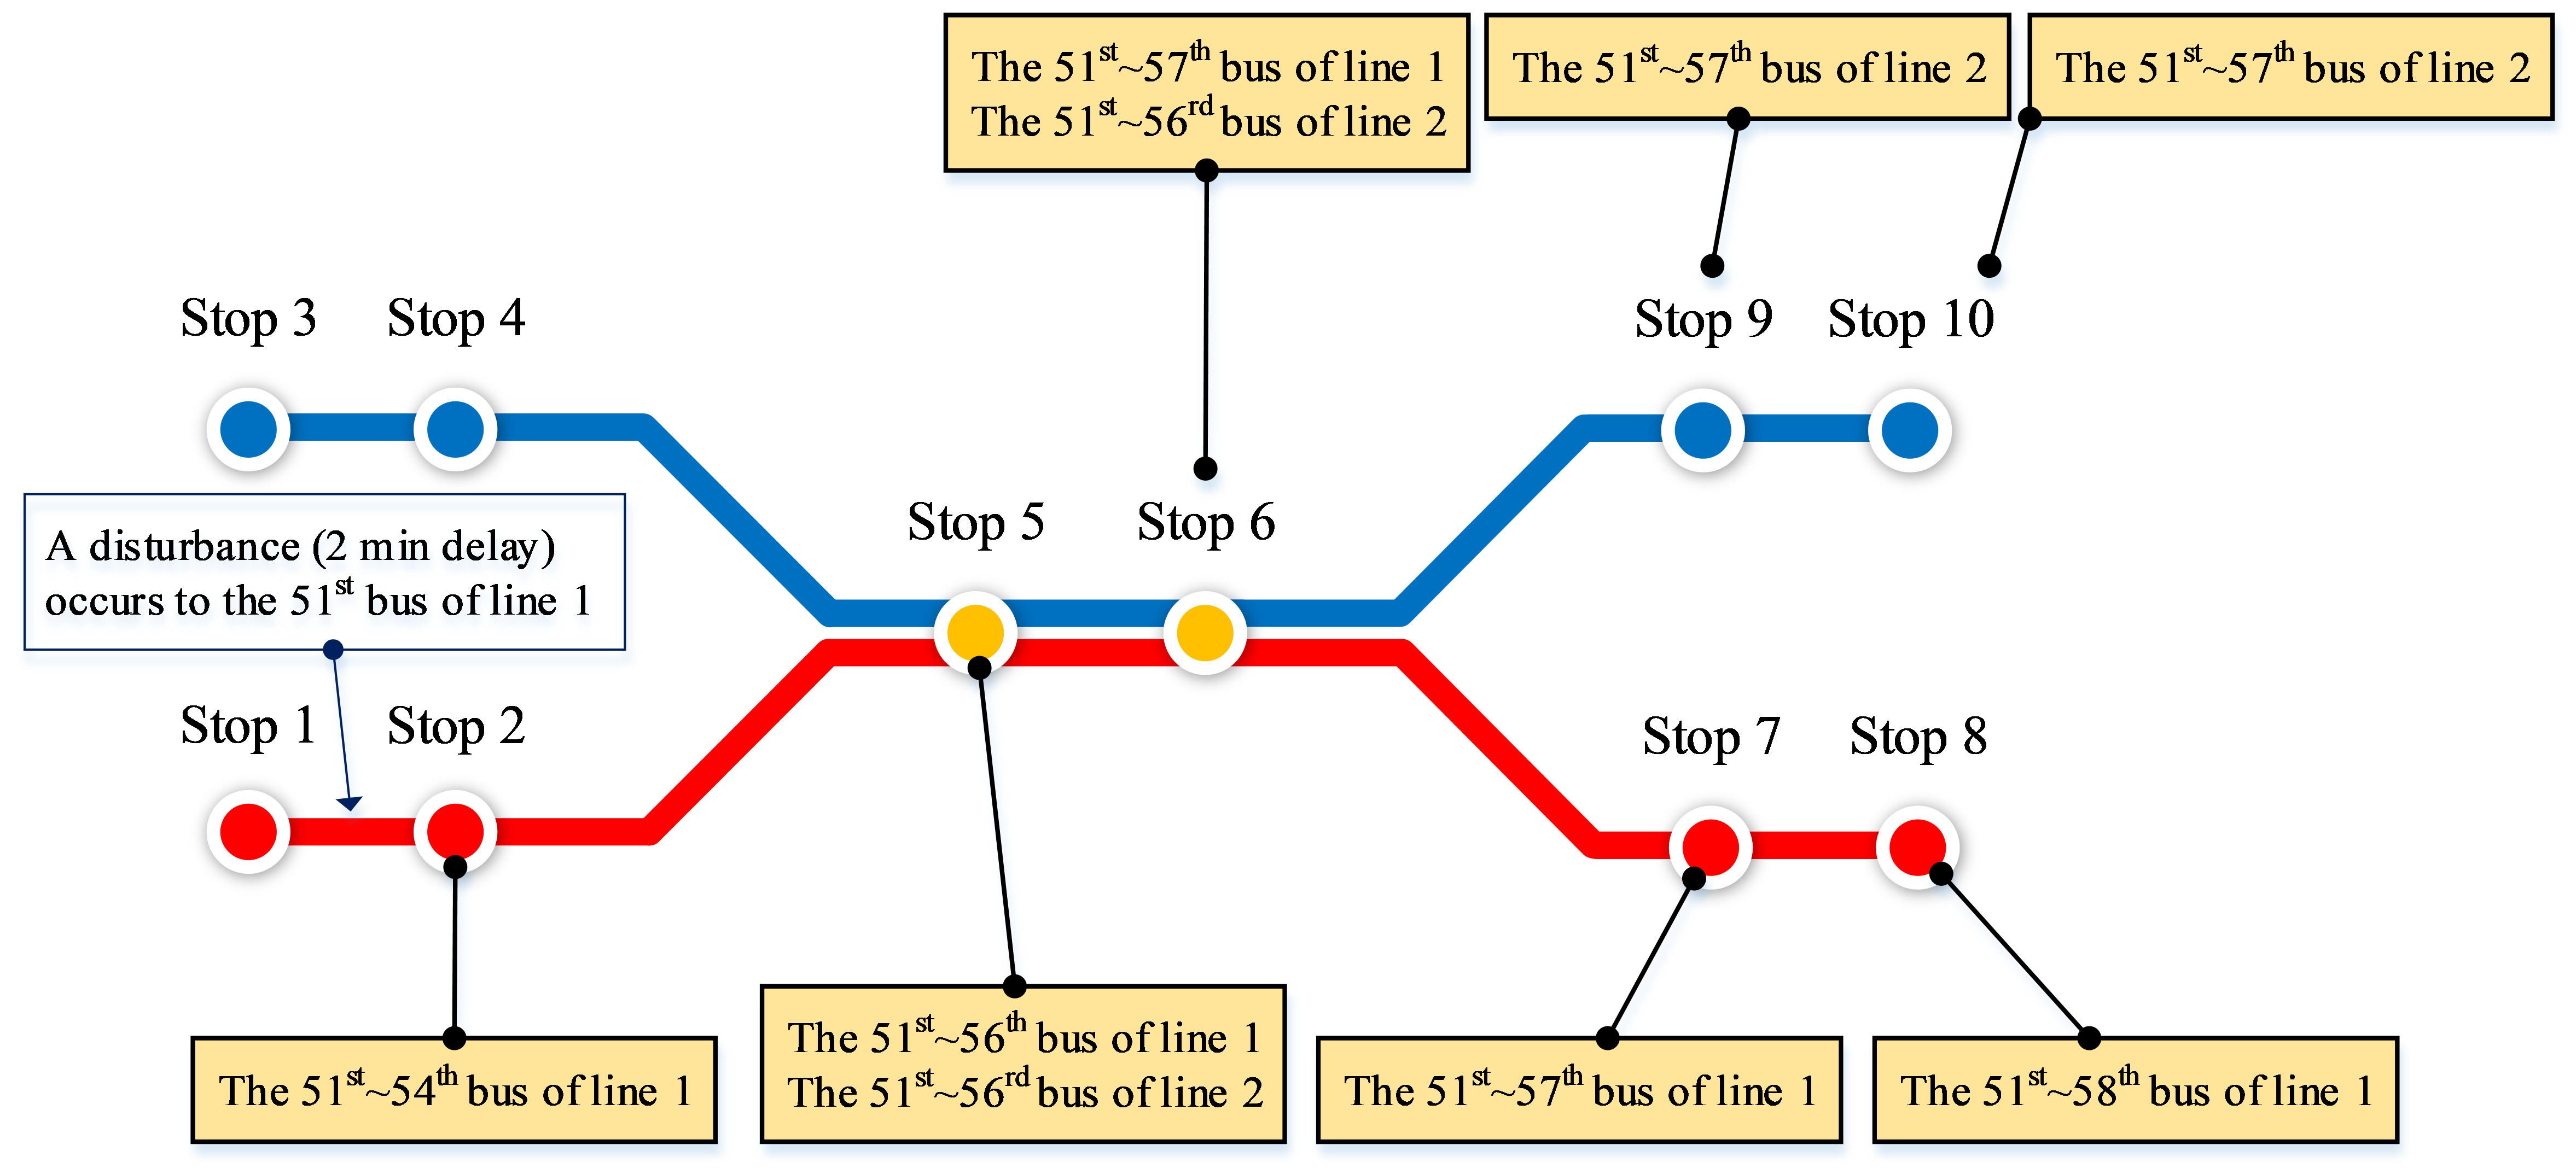
\includegraphics[width=0.9\linewidth]{CASPT2021paper_fig/range.png}
    \caption{A disturbance occurs to the $51^{st}$ bus of line 1 (red line) from stop 1 to stop 2 and subsequent buses and downstream stops are affected}
    \label{fig:range}
\end{figure}
The numbers of affected buses at stops reveal the temporal and spatial distribution of the effect of bus bunching.
As shown in Fig.\ref{fig:heatmap MSA and equal}, bus bunching problem is heavier in the downstream of the bus line and transfer passengers' routing based on real-time bus operation information makes bus bunching maintain longer time comparing with 
transfer passengers' routing based on historical or expected bus operation.
To facilitate the calculation of evaluation indices introduced following, 
we introduce a binary variable: 
\begin{equation}
    \begin{split}
        &x_{m,n}=
        \begin{cases}
            1&\text{ if the dwelling of bus } m \text{ at stop } n \text{ is affected;}\\
            0&\text{ otherwise.}
        \end{cases}\\
        &\forall m \in \mathcal{M}^{1}\cup\mathcal{M}^{2}; n \in \mathcal{S}^{1}\cup\mathcal{S}^{2}        
    \end{split}
\end{equation}
\subsection{Evaluation measurements}
We adopt two evaluation indexes: 
the average waiting time at stops and the standard deviation of bus time headway, which are commonly used 
as evaluation measurements and optimization objectives in related literature (i.e. Delgado et al., 2012; Hernández et al. 2015; Liang et al., 2016; Schmöcker et al., 2016; Wu et al., 2017).
The passengers waiting for bus $m$ of line $r$ at common stop $n$ can be divided into four groups:
\begin{enumerate}[1)]
    \item The passengers arrived after the departure of bus $m-1$ who take only line $r$.
    \item The passengers arrived before the departure of bus $m-1$ who take only line $r$.
    \item The passengers arrived after the departure of bus $m^{r,r'}(m,n)$ who take both line $r$ and line $r'$.
    \item The passengers arrived before the departure of bus $m^{r,r'}(m,n)$ who take both line $r$ and line $r'$.
\end{enumerate} 

Based on the constant arrival rates assumption in A2), 
the total waiting time of the four groups of passengers for bus $m$ of line $r$ can be estimated 
as $\frac{h_{m,n}^{r}}{2},h_{m,n}^{r},\frac{h_{m,n}^{r,r'}}{2}$ and $h_{m,n}^{r,r'}$ respectively. 
The total waiting time for bus $m$ of line $r$ at stop $n$ can be derived as: 
\begin{equation}
    w_{m,n}^{r} = \frac{1}{2}\Lambda_{n}^{r}\cdot {h_{m,n}^{r}}^{2} + \frac{1}{2}\Lambda_{n}^{r,r'}\cdot {h_{m,n}^{r,r'}}^{2}
    + L_{m-1,n}^{r} \cdot h_{m,n}^{r} + L_{m-1,n}^{r} \cdot h_{m,n}^{r}
\end{equation}
The average waiting time of passengers in study range can be calculated by: 
\begin{equation}
    \bar{w} = \frac{\sum\limits_{n\in \mathcal{S}^{1}\cup\mathcal{S}^{2}}\sum\limits_{m\in \mathcal{M}^{1}\cup\mathcal{M}^{2}} x_{m,n}\cdot w_{m,n}^{r}}
    {\sum\limits_{n\in \mathcal{S}^{1}\cup \mathcal{S}^{2}} \sum\limits_{m\in \mathcal{M}^{1}\cup \mathcal{M}^{2}}x_{m,n}\cdot \bar{B}_{m,n}}
\end{equation}

Similarly, the average waiting time of a single line $r$ can be calculated by:
\begin{equation}
    \bar{w}^{r} = \frac{\sum\limits_{n\in \mathcal{S}^{r}}\sum\limits_{m\in \mathcal{M}^{r}} x_{m,n}\cdot w_{m,n}^{r}}
    {\sum\limits_{n\in \mathcal{S}^{r}} \sum\limits_{m\in \mathcal{M}^{r}}x_{m,n}\cdot \bar{B}_{m,n}}
\end{equation}

The standard deviation of the time headway of affected buses of line $r$ is calculated by 
\begin{equation}
    \sigma^{r} = \sqrt{\frac{\sum\limits_{n\in \mathcal{S}^{r}}\sum\limits_{m\in \mathcal{M}^{r}} x_{m,n}\cdot \left(h_{m,n}^{r}-\bar{h}^{r}\right)^{2}}
    {\sum\limits_{n\in \mathcal{S}^{r}}\sum\limits_{m\in \mathcal{M}^{r}} x_{m,n}}}
\end{equation}
where $\bar{h}^{r}=\frac{\sum\limits_{n\in \mathcal{S}^{r}}\sum\limits_{m\in \mathcal{M}^{r}} x_{m,n}\cdot h_{m,n}^{r}}
{\sum\limits_{n\in \mathcal{S}^{r}}\sum\limits_{m\in \mathcal{M}^{r}} x_{m,n}}$ 
denotes the mean headway of line $r$ among affected buses.

\section{Numerical results and sensitivity analysis}\label{example}
To demonstrate the properties of the model, in this section, we use a small two-line transit network as an example to examine the effects of transfer behavior and capacity constraint on bus bunching. 

% \subsection{System specifications}\label{example specifications}
As shown in Fig.\ref{fig:example}, the network consists 10 stops divided into 5 stop sets:
$\mathcal{N}_{up}^{1}=\left\{1,2\right\},
\mathcal{N}_{up}^{2}=\left\{3,4\right\},
\mathcal{N}_{com}^{1,2}=\left\{5,6\right\},
\mathcal{N}_{down}^{1}=\left\{7,8\right\},
\mathcal{N}_{down}^{2}=\left\{9,10\right\}$. 
The constant bus departure intervals of two bus lines are set as $H^{1}=H^{2}=6$ (min), 
and the first bus of line 2 departs 3 min later than the first bus of line 1 
(i.e. $t^{1}=0,t^{2}=3$). 
All stops except the two terminals have the same passenger arrival rates as 5 pas/min 
(i.e. $\Lambda_{n}=5$ for $n\in \mathcal{S}^{1}\cup\mathcal{S}^{2}\backslash\left\{8,10\right\}$).
The arrival rate at each stop is divided evenly among all destination stops:
\begin{equation}
    \label{equ:lambda}
    \lambda_{n,j} = \frac{\Lambda_{n}}{\left|\mathcal{S}^{D}(n)\right|};
    \forall j\in \mathcal{S}^{D}(n);n\in\mathcal{S}^{1}\cup\mathcal{S}^{2}\backslash\left\{n^{1}_{\left|\mathcal{S}^{1}\right|},n^{2}_{\left|\mathcal{S}^{2}\right|}\right\}
\end{equation}
% For example, the set of destination stops of stop 1 in \textup{Fig.\ref{fig:example}} is 
% $\mathcal{S}^{D}(1)=\left\{2,5,6,7,8,9,10\right\}$. 
% As the total arrival rate at stop 1 is set as $\Lambda_{1} = 5$ pas/min, 
% the passenger arrival rate with destination stop $j$ is 
% $\lambda_{1,j}=\frac{\Lambda_{1}}{\left|\mathcal{S}^{D}(1)\right|}=\frac{5}{7},j\in\mathcal{S}^{D}(1)$. 
The travel times for all buses in each link between stops are set as 3 min 
(i.e. $T_{m,n}=3,m\in\mathcal{M}^{1}\cup \mathcal{M}^{2},n\in \mathcal{S}^{1}\cup\mathcal{S}^{2}\backslash \left\{8,10\right\}$).
% forget to say cap=100
\begin{figure}[H]
    \centering
    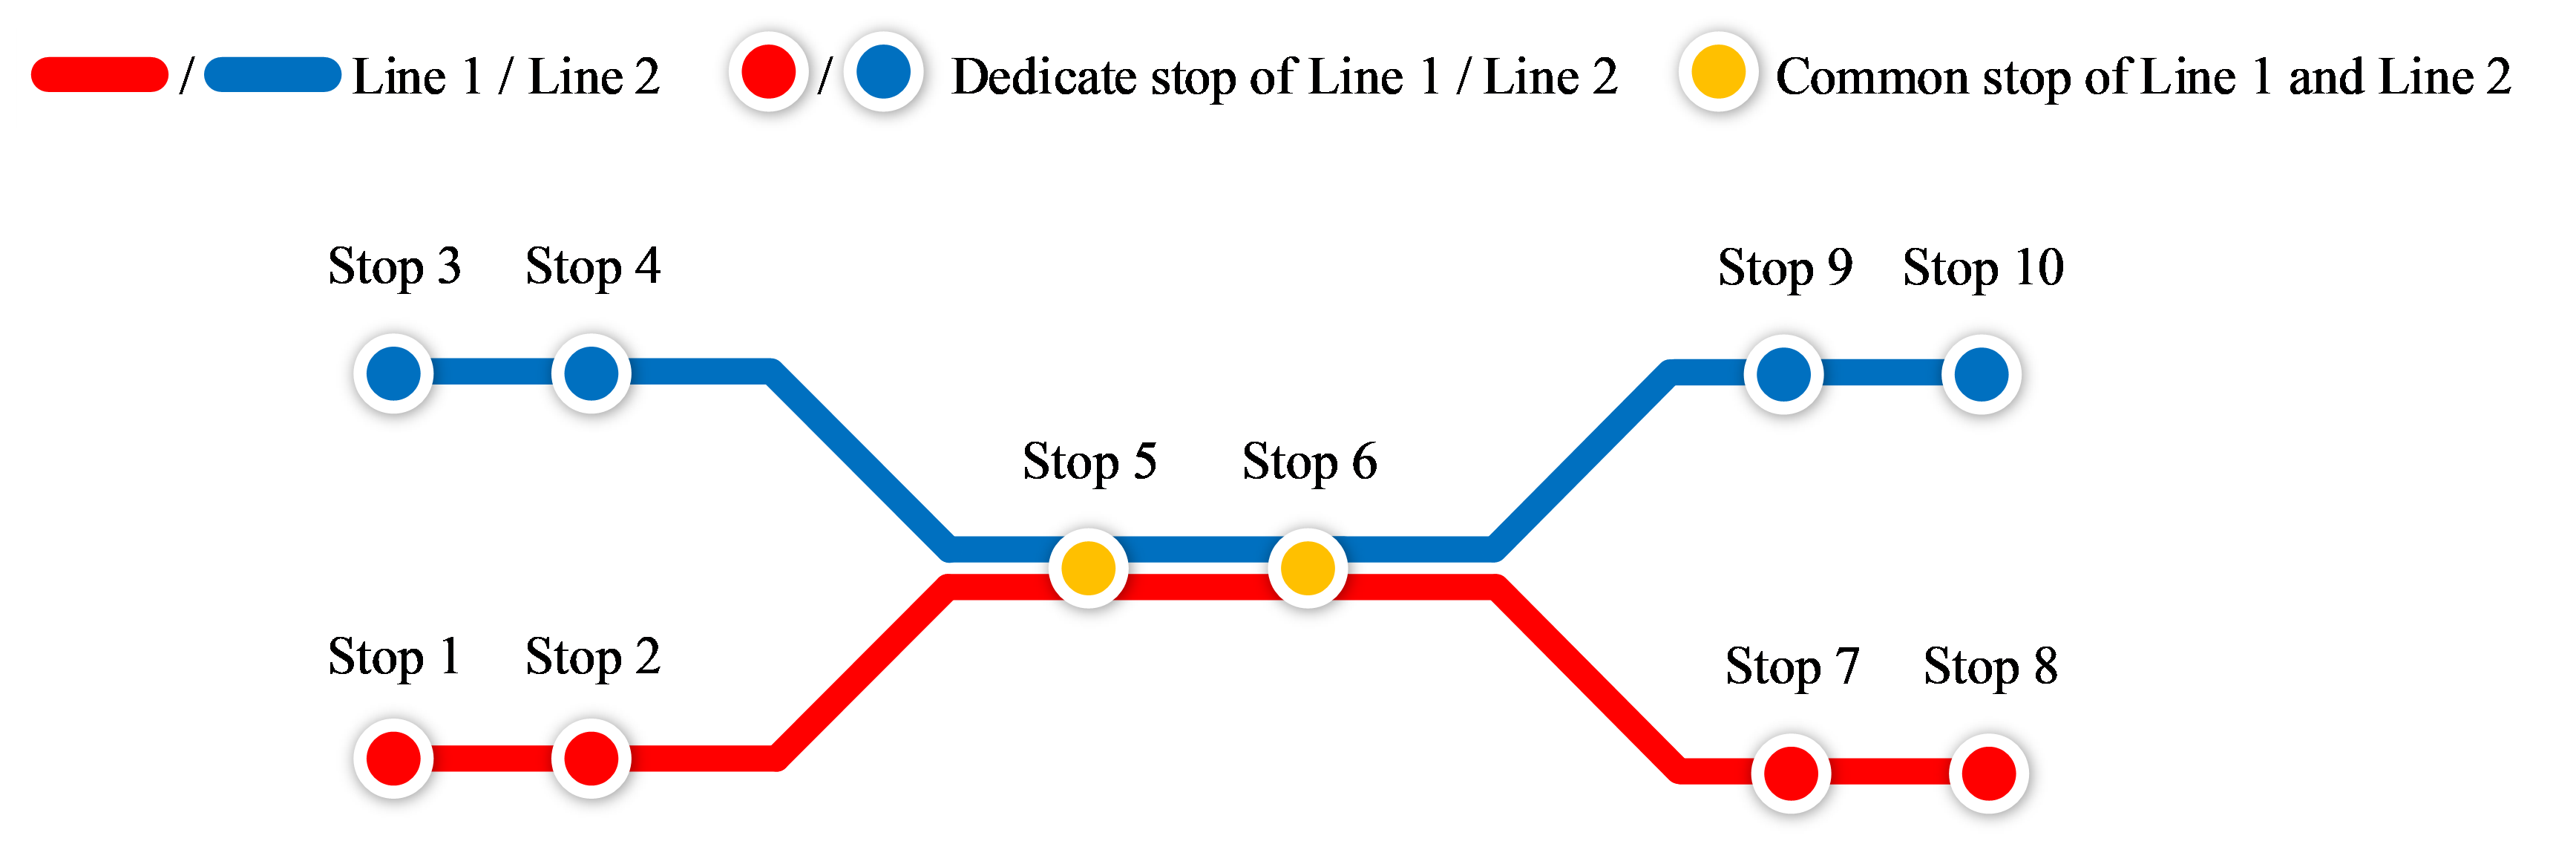
\includegraphics[width=1\linewidth]{CASPT2021paper_fig/Fig2.png}
    \caption{An example of two-line systems with 10 stops}
    \label{fig:example}
\end{figure}

\subsection{Effect of transfer behaviors}\label{subsec: effc of trafer behaviors}
This experiment is designed to investigate the effect of considering passegners transfer behavior in modelling bus bunching. We consider two scenarios, a benchmark scenario and a bus bunching scenario, where a 2 minutes delay is introduced to one bus of line 1 between stop 1 and stop 2 to trigger the bus bunching. 
In this scenario, we further compute two cases, a non re-routing and a re-routing case, where the former one does not allow passengers to adjust their routes, while the latter one allows and determines the transfer passengers via the proposed transfer equilibrium model.

Fig.\ref{fig:uniform trajectories} shows bus trajectories obtained from the benchmark scenario in time-space diagram, in which the horizontal axis corresponds to the sequence of stops along the line.
The figure shows that buses run steadily and there is no bus full-loaded.
Routing result of transfer passengers shown in Fig.\ref{fig:uniform alpha up},\ref{fig:uniform alpha down} 
demonstrates that the equilibrium assignment degenerates to the equal assignment 
(i.e. $\alpha_{5}^{m}=\alpha_{6}^{m}=0.5$ for $m\in\mathcal{M}^{1}\cup\mathcal{M}^{2}$) as a specific example verifying Proposition \ref{pro:equal assignment}.

\begin{figure}[H]
    \centering
    \begin{tabular}{m{6cm}c}
        \subfloat[Undisturbed bus trajectories]{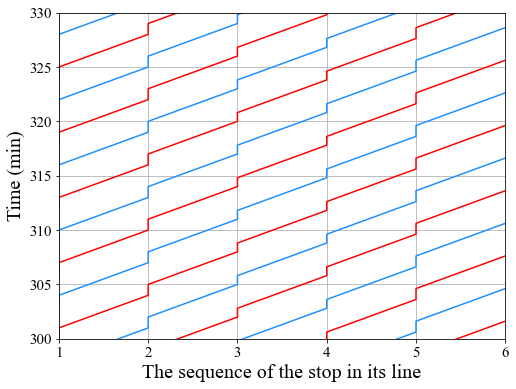
\includegraphics[width=0.45\textwidth\label{fig:uniform trajectories}]{CASPT2021paper_fig/uniform trajectories.png}} 
        & \makecell{\subfloat[$\alpha_{5}^{m}$ and $\alpha_{6}^{m}$ for bus $m$ of line 1]{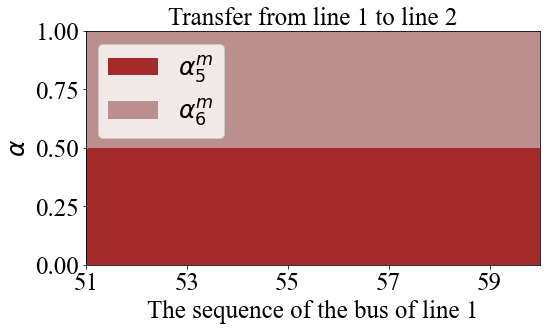
\includegraphics[width=0.4\textwidth\label{fig:uniform alpha up}]{CASPT2021paper_fig/uniform alpha of line 1 (short).png}}\\
        \subfloat[$\alpha_{5}^{m}$ and $\alpha_{6}^{m}$ for bus $m$ of line 2]{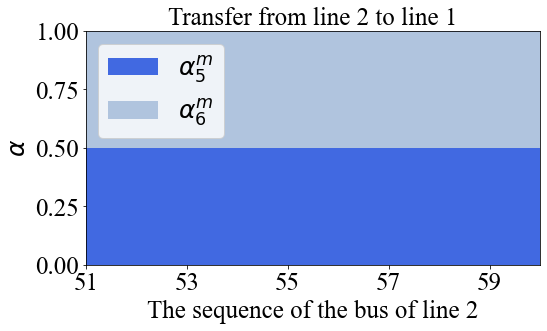
\includegraphics[width=0.4\textwidth\label{fig:uniform alpha down}]{CASPT2021paper_fig/uniform alpha of line 2 (short).png}}} 
        \end{tabular}
        \caption{Undisturbed bus trajectories and routing result of transfer passengers}
\end{figure}

\textcolor{red}{
    TO revise
    first, describes the figure, explain the figure, implication of the figure
}

The routing result of transfer passengers shown in Fig.\ref{fig:uniform alpha up},\ref{fig:uniform alpha down} represents a routing behavior based on the expected bus operation without disturbance.
If there is a recurrent delay or a long-lived control strategy in bus operation, the routing behaviors of transfer passengers tend to a new equilibrium.
As a comparison, when the system encounters an accidental delay or an interim control strategy, 
the routing behaviors of transfer passengers onboard won't form an equilibrium as they are not informed with the operation.
We introduce a 2 min travel delay occurring to one bus of line 1 between stop 1 and stop 2, 
and the bus dwellings at subsequent stops of this line and downstream stops of the other line could be involved in a bunching problem. 
As shown in Fig.\ref{fig:disturbed MSA and equal}, the buses trajectories and transfer passengers' routing results are different under a recurrent delay.
The deviations of bus trajectories casused by the delay is shown in Fig.\ref{fig:heatmap MSA and equal}.
It demonstrates that a recurrent delay may cause heavier bus bunching problem maintaining longer time and affecting more buses than
transfer passengers' routing behavior  bus operations makes different impacts on bus bunching 
comparing with that based on their expected bus operation.\newpage

\begin{figure}[H]
\centering
% \begin{tabular}{|c|c|}
\begin{tabular}{|p{5cm}|p{5cm}|}
    \hline
     \textcolor{white}{aaaaaa}\textbf{Equilibrium for a recurrent delay} & \textcolor{white}{aaa}\textbf{No equilibrium for an accidental dealy} \\
    \hline
    \subfloat[$\alpha_{5}^{m}$ and $\alpha_{6}^{m}$ for bus $m$ of line 1 ]
    {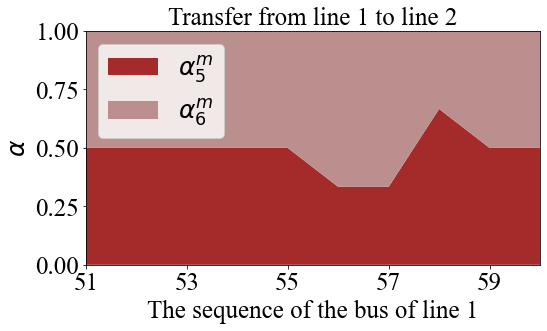
\includegraphics[width=0.4\textwidth\label{fig:disturbed MSA alpha up}]{CASPT2021paper_fig/disturbed alpha of line 1 (short).png}} 
    & \subfloat[$\alpha_{5}^{m}$ and $\alpha_{6}^{m}$ for bus $m$ of line 1 ]
    {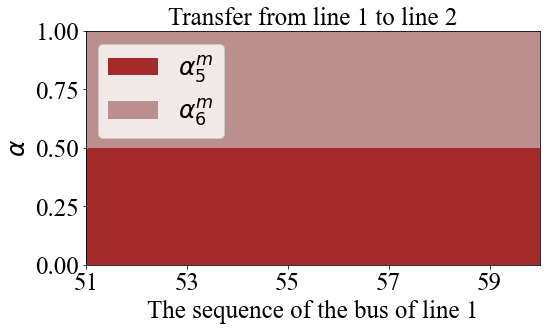
\includegraphics[width=0.4\textwidth\label{fig:disturbed equal alpha up}]{CASPT2021paper_fig/uniform alpha of line 1 (short).png}} \\ \hline

    \subfloat[$\alpha_{5}^{m}$ and $\alpha_{6}^{m}$ for bus $m$ of line 2 ]
    {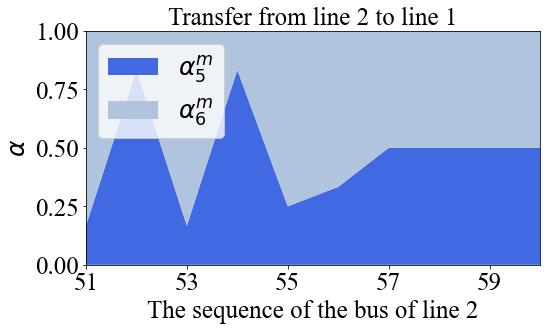
\includegraphics[width=0.4\textwidth\label{fig:disturbed MSA alpha down}]{CASPT2021paper_fig/disturbed alpha of line 2 (short).png}} 
    & \subfloat[$\alpha_{5}^{m}$ and $\alpha_{6}^{m}$ for bus $m$ of line 2]
    {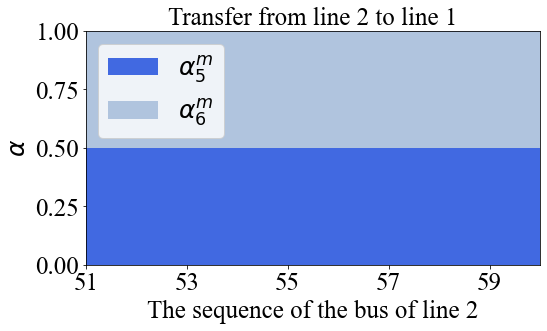
\includegraphics[width=0.4\textwidth\label{fig:disturbed equal alpha down}]{CASPT2021paper_fig/uniform alpha of line 2 (short).png}} \\ \hline
    \subfloat[Bus trajectories under a recurrent delay]
    {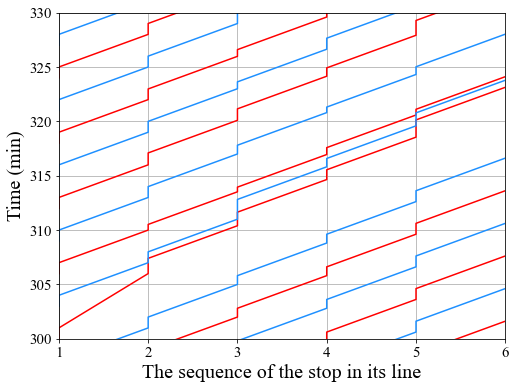
\includegraphics[width=0.4\textwidth\label{fig:disturbed MSA trajectories}]{CASPT2021paper_fig/disturbed MSA trajectories.png}} 
    & \subfloat[Bus trajectories under a accidental delay]
    {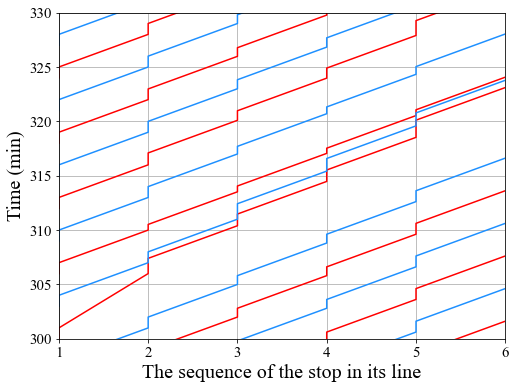
\includegraphics[width=0.4\textwidth\label{fig:disturbed equal trajectories}]{CASPT2021paper_fig/disturbed equal trajectories.png}} \\ \hline
    \end{tabular}
    \caption{Different transfer routing results and bus trajectories under a recurrent delay and an accidental delay}
    \label{fig:disturbed MSA and equal}
\end{figure}

\begin{figure}[H]
\centering
\begin{tabular}{|c|c|}
    \hline
    Deviation caused by a recurrent 2 min delay & Deviation caused by an accidental 2 min delay \\ \hline
    \subfloat[Deviation times of line 1 ]
    {\includegraphics[width=0.4\textwidth\label{fig:MSA heatmap 1}]{experiments/experiment 1:affected bus dwell events of line 1.png}} 
    & \subfloat[Deviation times of line 1 ]
    {\includegraphics[width=0.4\textwidth\label{fig:equal heatmap 1}]{experiments/experiment 2:affected bus dwell events of line 1.png}} \\ \hline

    \subfloat[Deviation times of line 2 ]
    {\includegraphics[width=0.4\textwidth\label{fig:MSA heatmap 2}]{experiments/experiment 1:affected bus dwell events of line 2.png}}
    & \subfloat[Deviation times of line 2 ]
    {\includegraphics[width=0.4\textwidth\label{fig:equal heatmap 2}]{experiments/experiment 2:affected bus dwell events of line 2.png}} \\ \hline
\end{tabular}
\caption{Different deviations of bus dwell times caused by a recurrent delay and an accidental delay}
\label{fig:heatmap MSA and equal}
\end{figure}
\textcolor{red}{rewrite the following}
What's more, we conduct numerical experiments to confirm the effect of the presence of transfer passenger flow on bus bunching. 
First, we introduce a transfer parameter $\mu \geq 0$ to adjust the proportion of transfer passengers among all passenger demand. 
For example, let us consider the $i^{th}$ upstream stop of line $r$ (i.e. $n=n^{r}_{i}$). 
As the destination stops set of stop $n$ is 
$\mathcal{S}^{D}(n)=\mathcal{S}^{D}({n}^{r}_{i})=\left\{n^{r}_{i}|n^{r}_{k}\in\mathcal{S}^{r},k>i\right\}\cup\mathcal{N}_{down}^{r'}$, 
we calculate the passenger arrival rate with the destination stop $j$ by
\begin{equation}
    \lambda_{n,j}=
    \begin{cases}
        \frac{\Lambda_{n}}{\left|\left\{n^{r}_{k}|n^{r}_{k}\in\mathcal{S}^{r},k>i\right\}\right|+\mu \cdot \left|\mathcal{N}_{down}^{r'}\right|}
        &j\in \left\{n^{r}_{k}|n^{r}_{k}\in\mathcal{S}^{r},k>i\right\}\\
        \frac{\mu \cdot \Lambda_{n}}{\left|\left\{n^{r}_{k}|n^{r}_{k}\in\mathcal{S}^{r},k>i\right\}\right|+\mu \cdot \left|\mathcal{N}_{down}^{r'}\right|}
        &j\in \mathcal{N}_{down}^{r'}
    \end{cases}
\end{equation}
In this way, the proportion of transfer passengers increases with $\mu$
while the total arrival rate calculated by \textup{Eq.(\ref{equ:sumLambda})} remains constant. 
There are two special cases: 
\begin{enumerate}[1)]
    \item when $\mu=0$, there is no transfer passengers between two lines. 
    \item when $\mu=1$, the composition of arrival passengers degenerates to the basic pattern as \textup{Eq.(\ref{equ:lambda})}.
\end{enumerate}

We set two conditions as $\mu=0$ and $\mu=5$ for a comparison and the bus trajectories are shown in the Fig.\ref{fig:disturbed mu=0} and Fig.\ref{fig:disturbed mu=5}. 
It is observed that the bus of line 2 (i.e. blue lines) following the disturbed bus of line 1 (i.e. red lines) 
is barely affected in the system with no transfer passengers but heavily affected in the second condition. 
The comparison demonstrates that 
the presence of transfer passenger flow enhances the propagation of bus bunching problem between bus lines.
\begin{figure}[H]
    \centering
    \begin{tabular}{cc}
        \subfloat[Disturbed bus trajectories with $\mu = 0$]{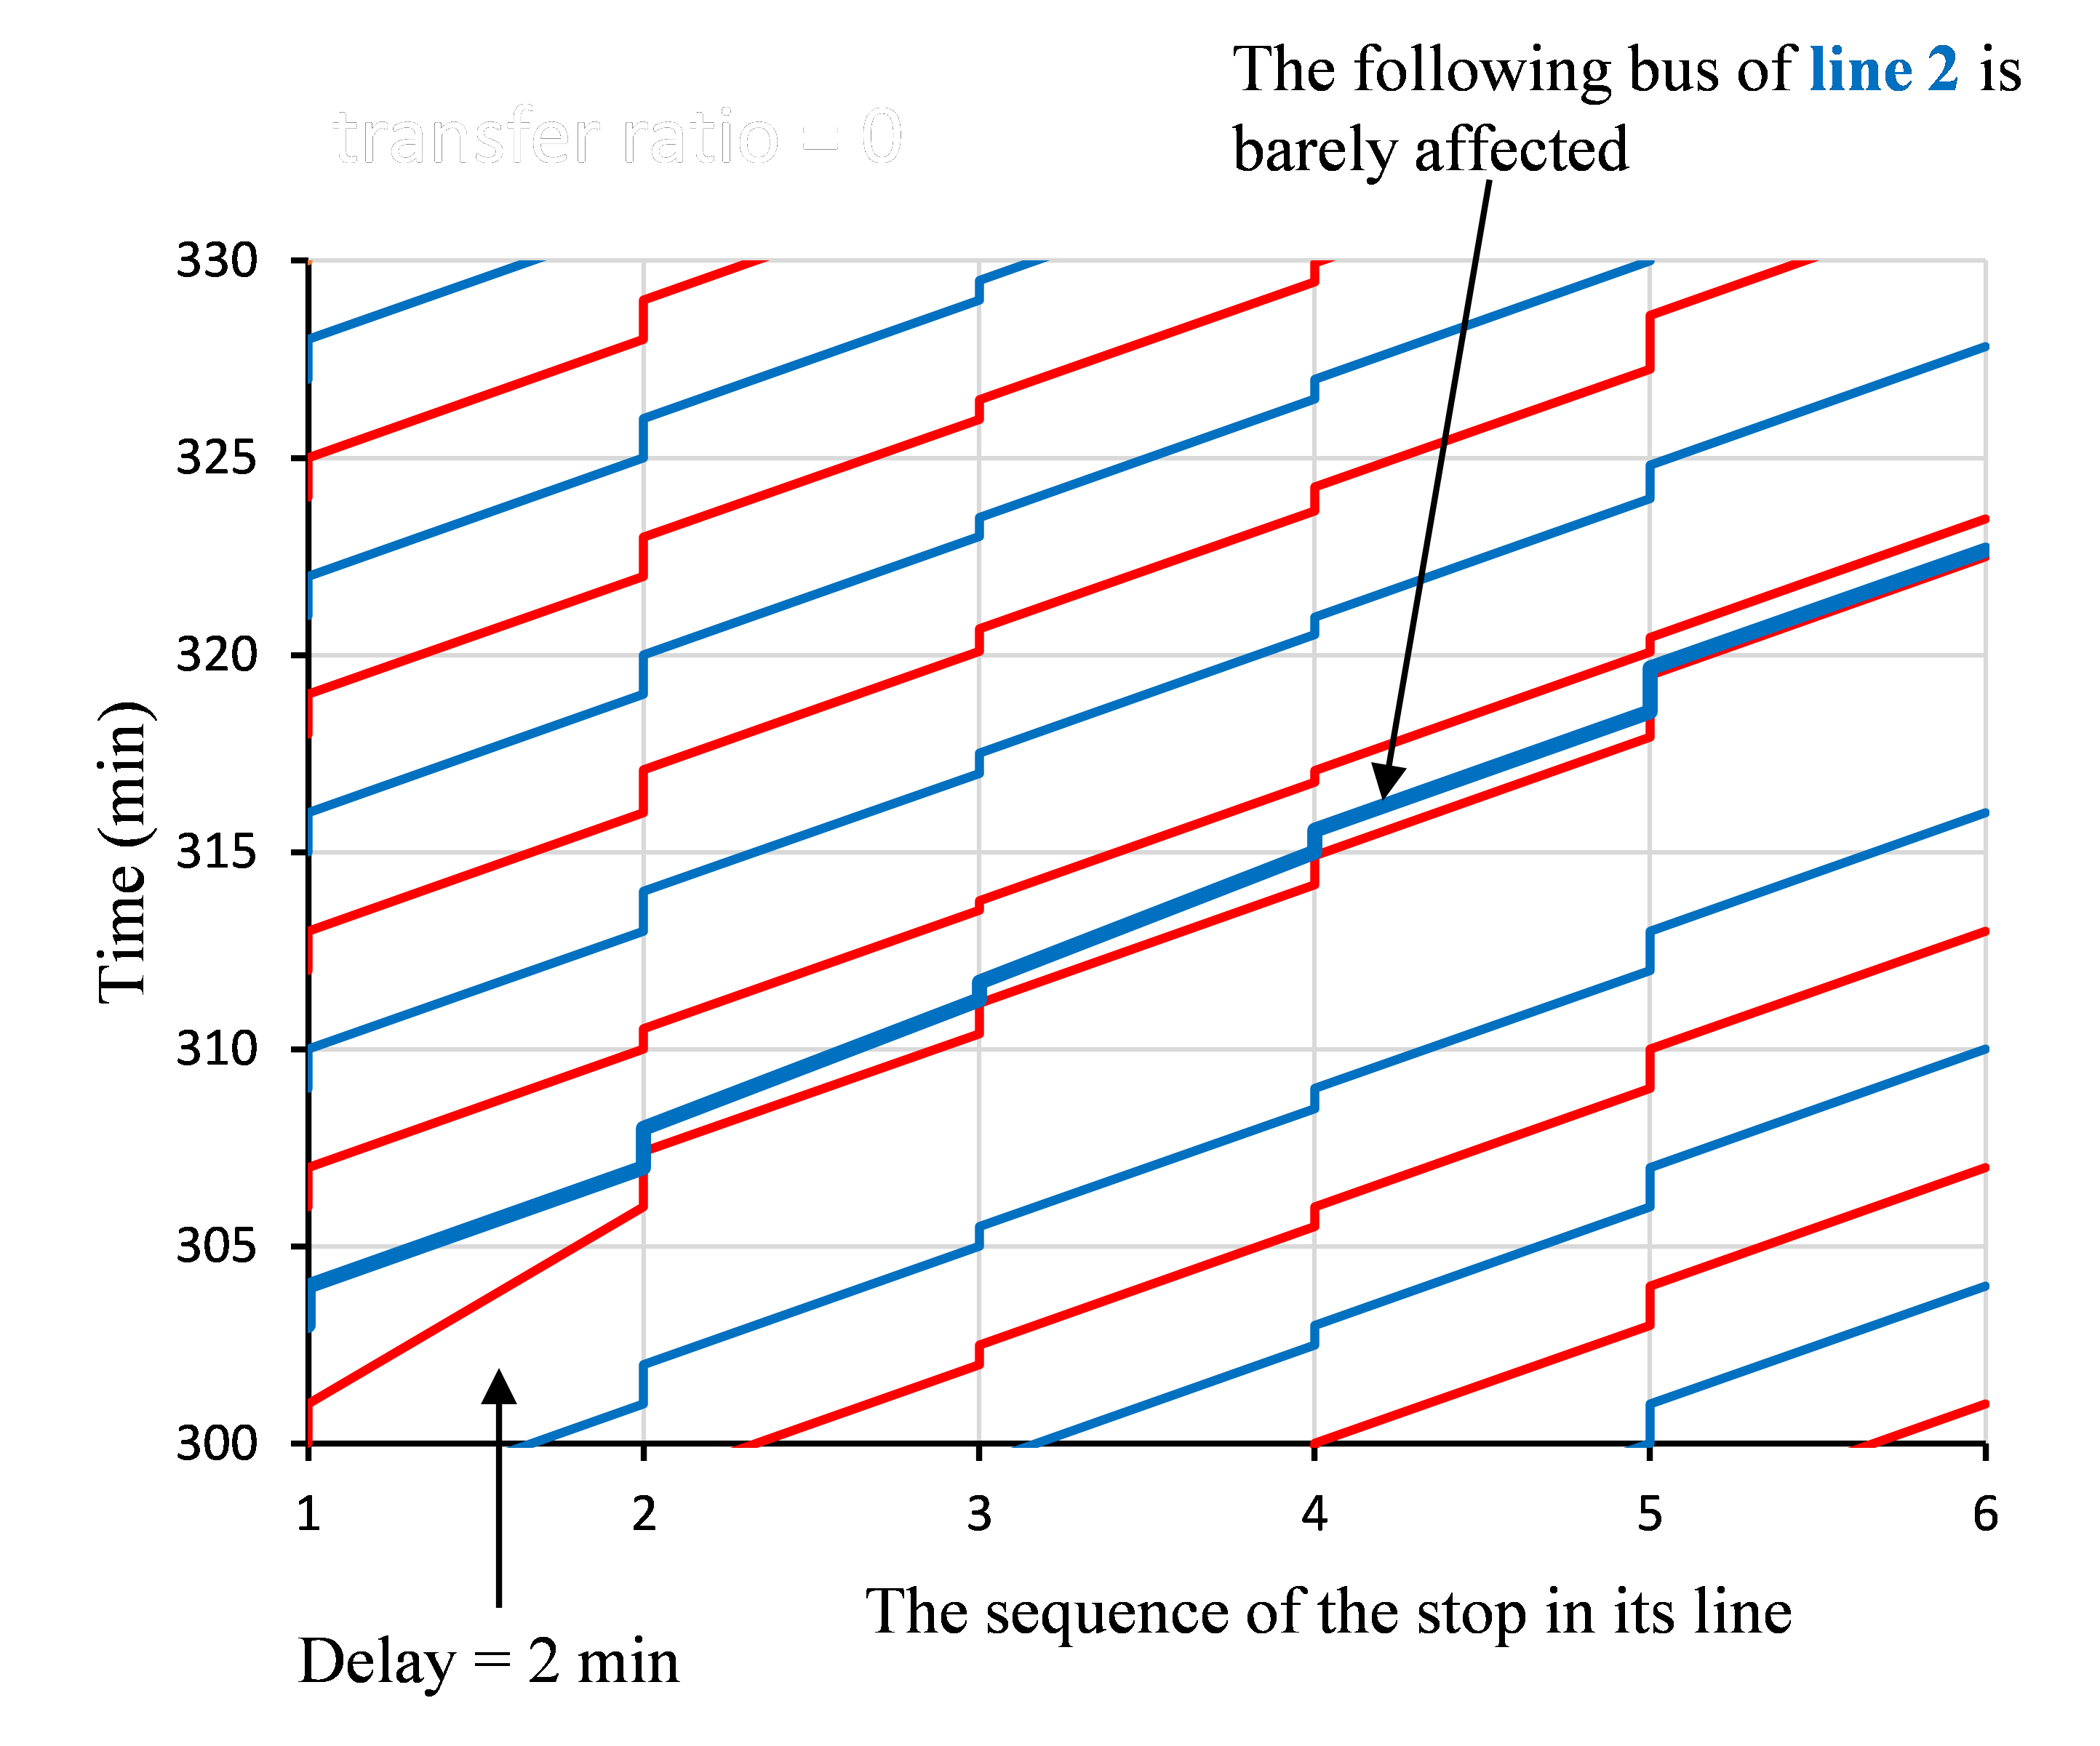
\includegraphics[width=0.45\textwidth\label{fig:disturbed mu=0}]{CASPT2021paper_fig/effect of transfer parameter 0.png}}
        &\subfloat[Disturbed bus trajectories with $\mu = 5$]{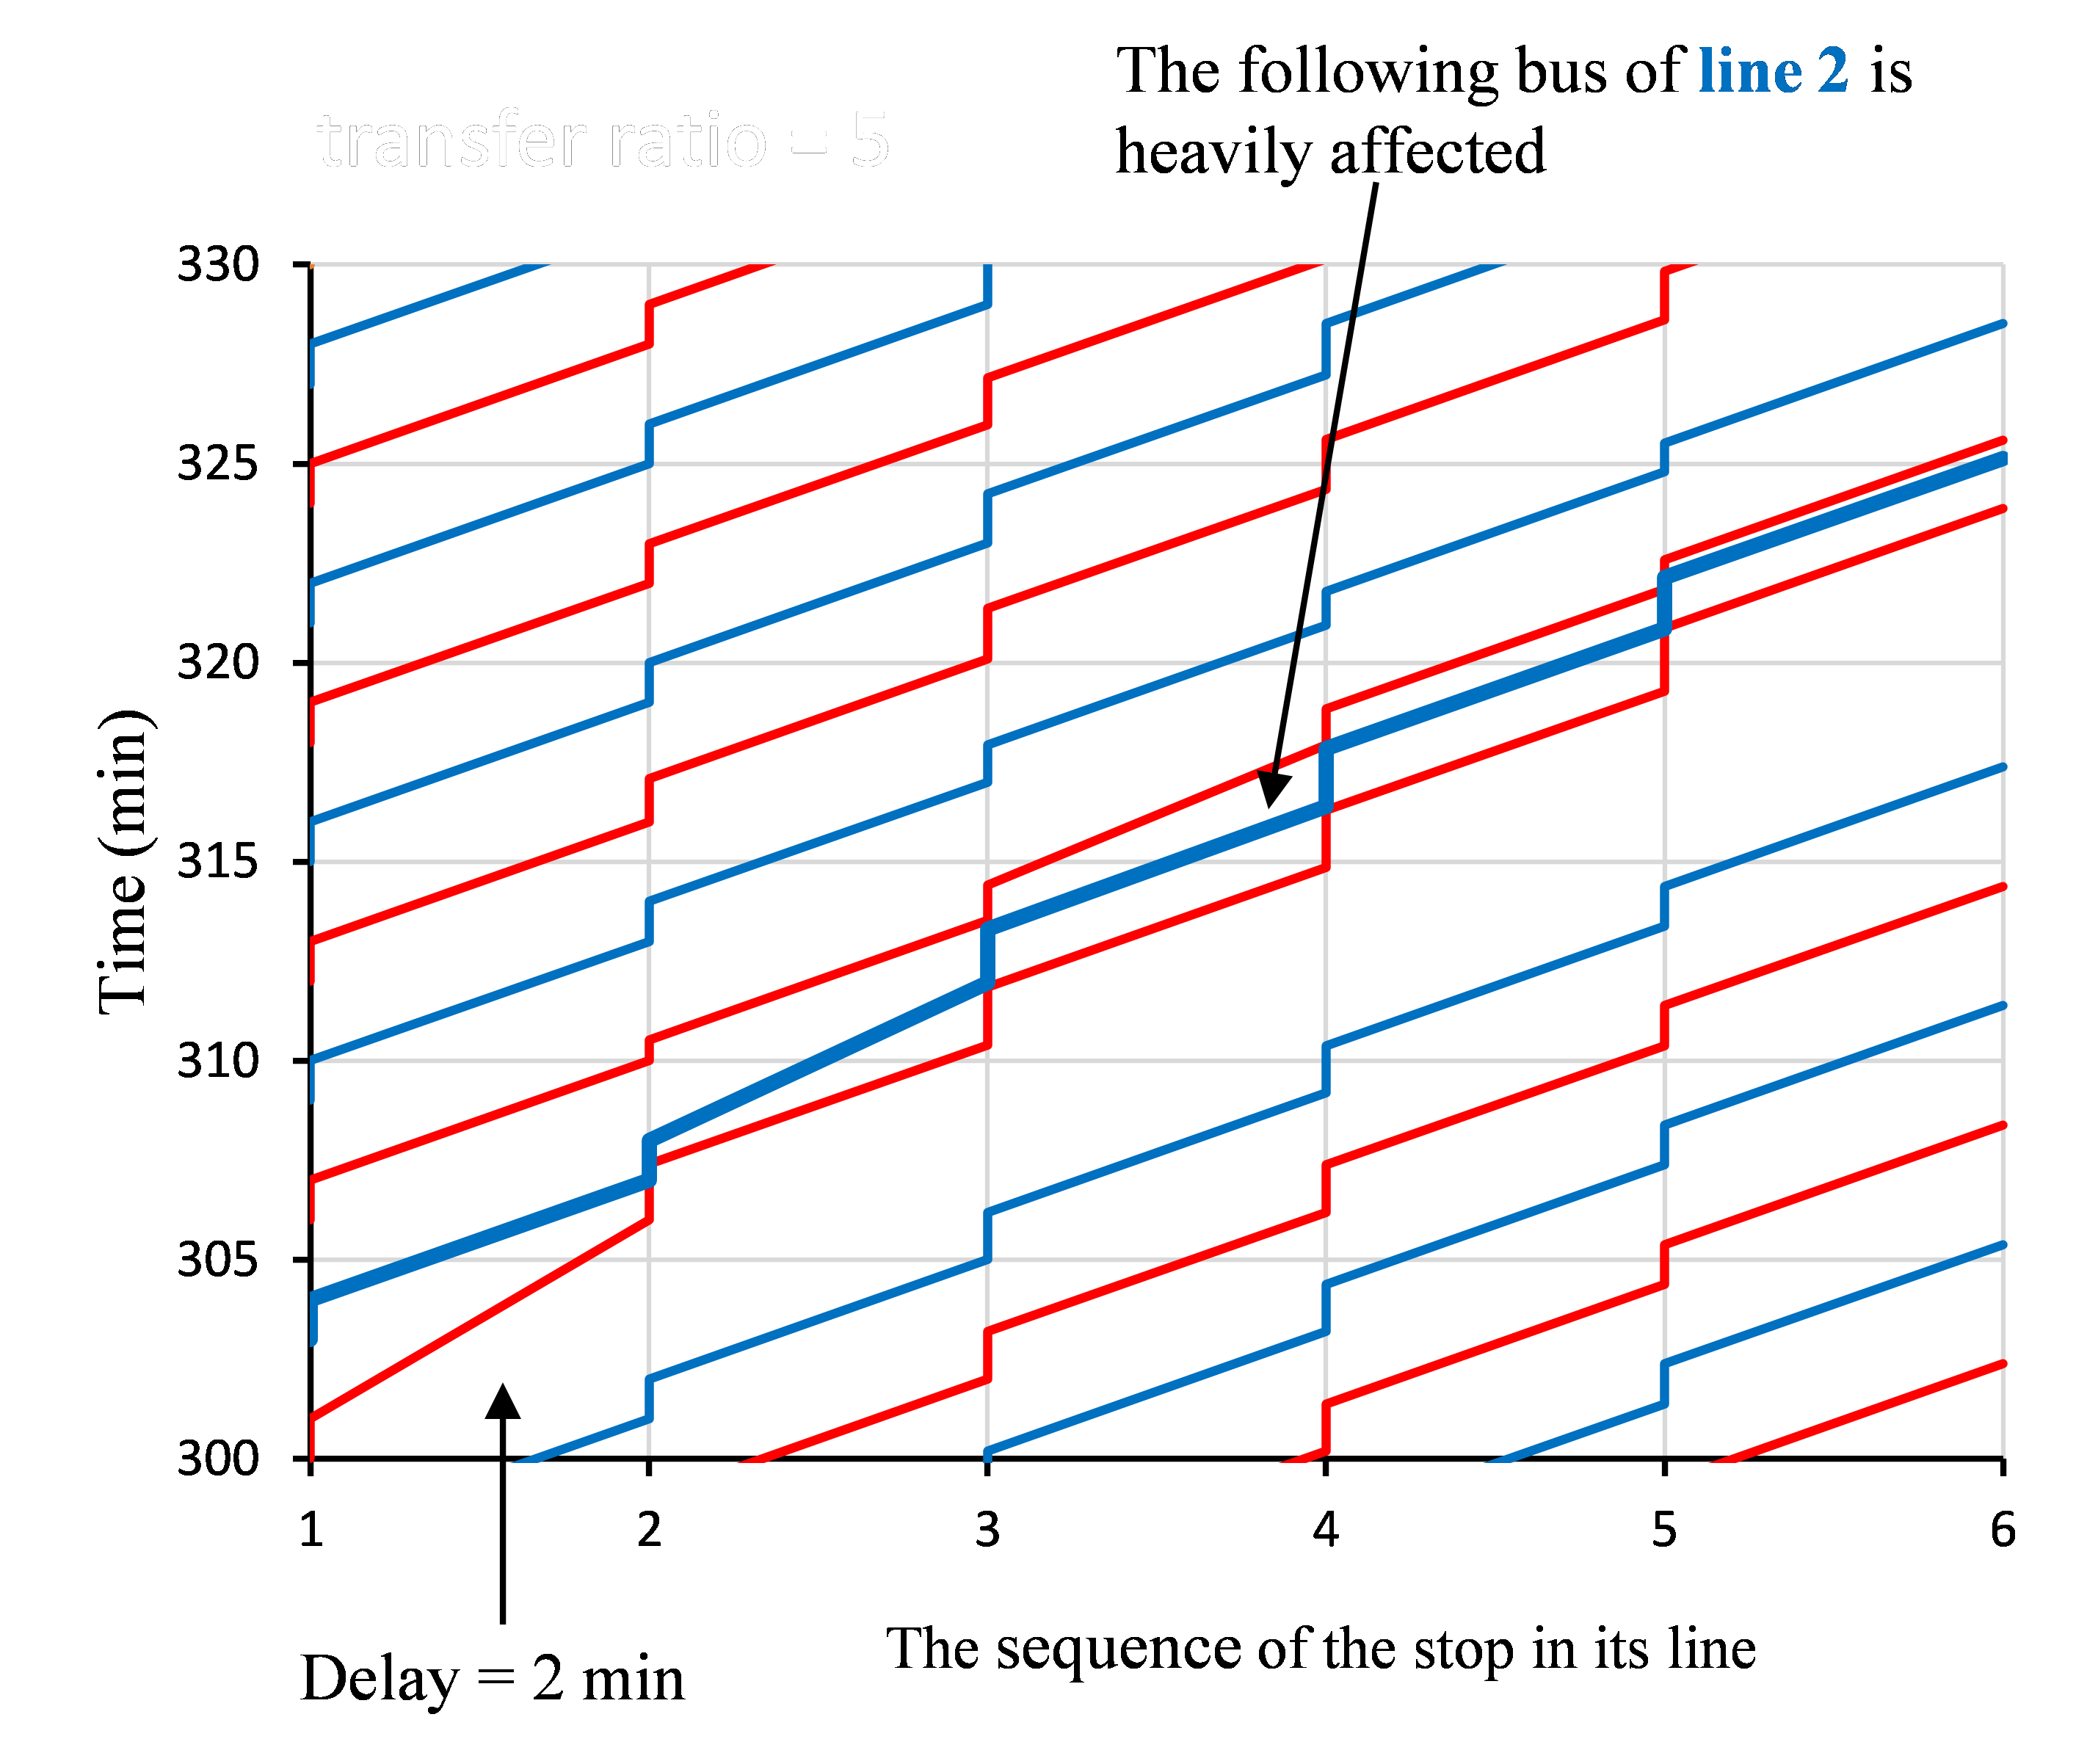
\includegraphics[width=0.45\textwidth\label{fig:disturbed mu=5}]{CASPT2021paper_fig/effect of transfer parameter 5.png}}
    \end{tabular}
    \caption{Effect of different transfer parameters}
\end{figure}

\subsection{Effect of capacity constraint}
We devise a comparison between two different capacity settings 
, 150 pas per bus and 80 pas per bus,
% (i.e. $cap_{m}=100,m\in\mathcal{M}^{1}\cup\mathcal{M}^{2}$) 
%(i.e. $cap_{m}=70,m\in\mathcal{M}^{1}\cup\mathcal{M}^{2}$)
while other parameters specified in \ref{example specifications} remain the same. 
The bus trajectories obtained are shown in Fig.\ref{fig:disturbed cap=150} and Fig.\ref{fig:disturbed cap=80}, respectively. 
The two figures demonstrate that the bus bunching phenomenon under different capacity settings are significantly different. Specifically, there are three buses bunching at the common corridor 
(i.e. when a bus arrives at the bus stop, the preceding bus is still at the bus stop) 
when the bus capacities are set as 150 pas, while only two buses are observably involved when the bus capacities are set as 80 pas. 
As we mentioned in \ref{barB}, the bus capacity is the upper bound of the number of onboard passengers 
and limits the bus dwell time at stops when a bus encounters a large boarding demand caused by bus bunching.
\begin{figure}[H]
  \centering
  \begin{tabular}{cc}
      \subfloat[Disturbed bus trajectories with $cap = 150$ (pas)]{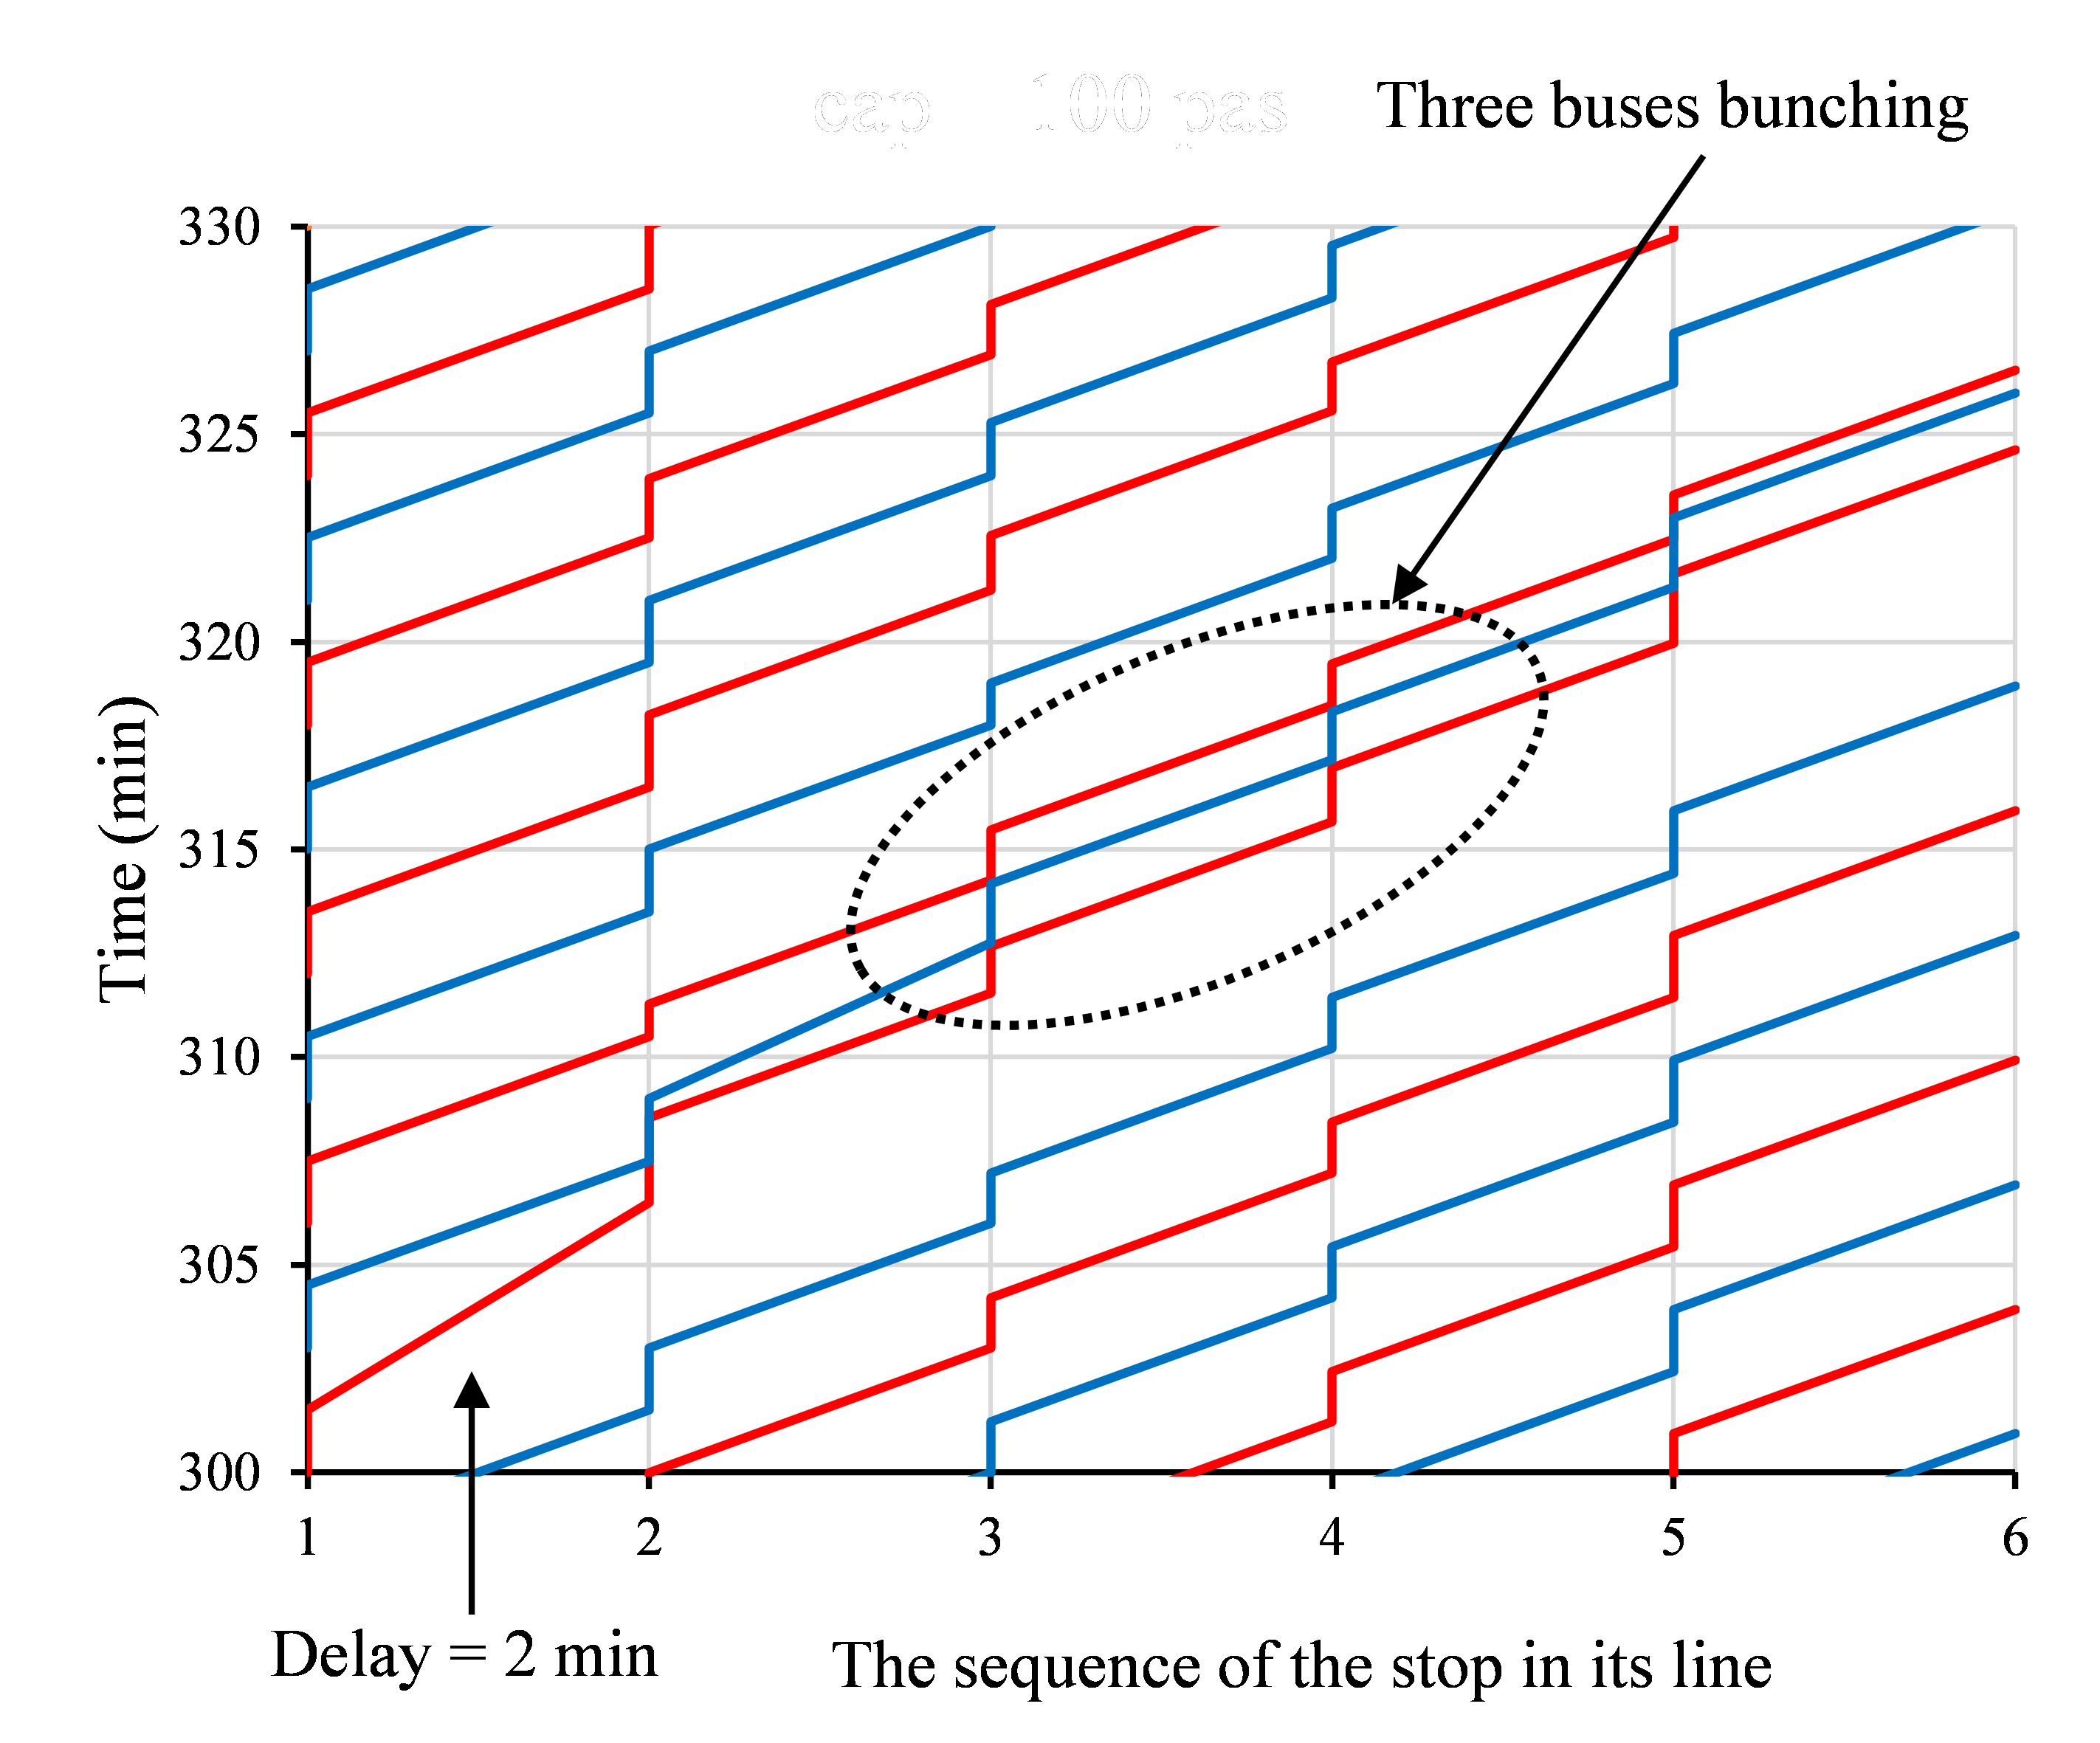
\includegraphics[width=0.45\textwidth\label{fig:disturbed cap=150}]{CASPT2021paper_fig/effect of capacity 100.png}}
      &\subfloat[Disturbed bus trajectories with $cap = 80$ (pas)]{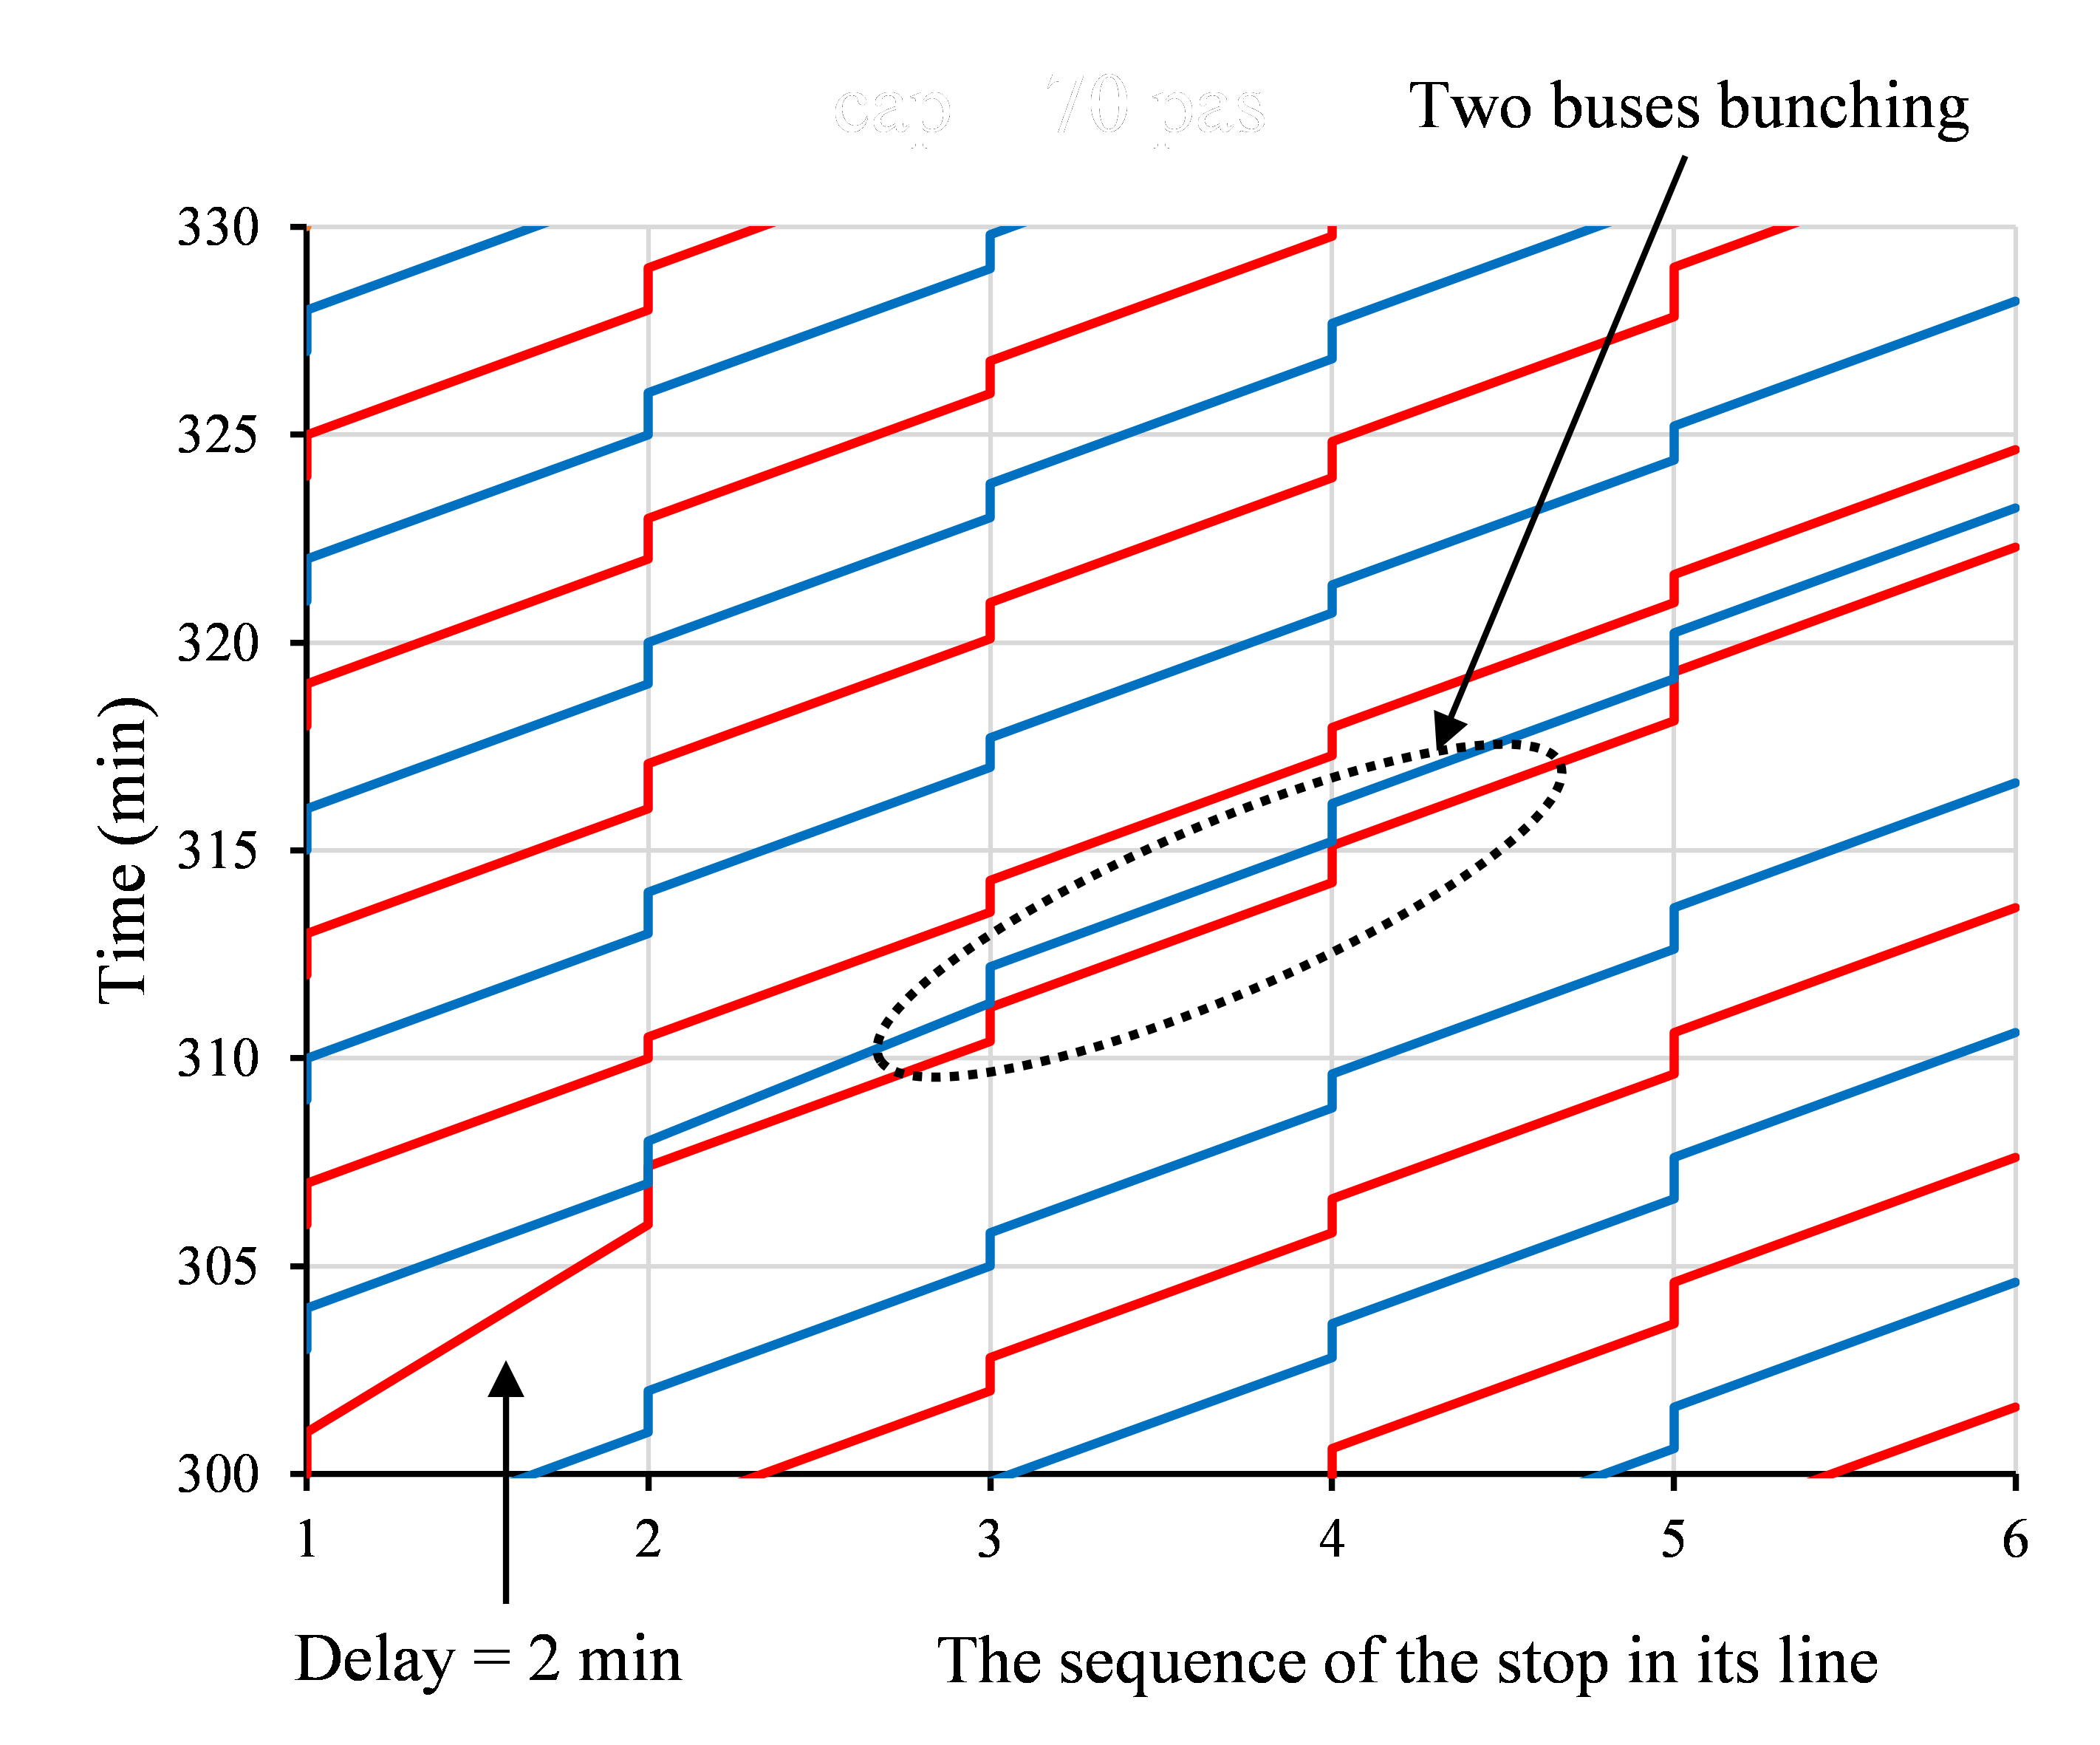
\includegraphics[width=0.45\textwidth\label{fig:disturbed cap=80}]{CASPT2021paper_fig/effect of capacity 70.png}}
  \end{tabular}
  \caption{Effect of different capacity settings}
  \label{fig:two cap}
\end{figure}
% \newpage
% \section{Performance evaluation and sensitivity analyses}\label{Evaluation and sensitivity analyses}

% \subsection{Sensitivity analysis}\label{sensitivity}
\subsection{Sensitivity analysis}\label{sensitivity}
Sensitive analysis is carried out to demonstrate the impacts of bus capacity and transfer flows on the bus bunching.
Considering a busy system with high demands and high-frequency services, 
we set the network structure as 
$\left| \mathcal{N}_{up}^{1}\right|=
\left| \mathcal{N}_{up}^{2} \right|=
\left| \mathcal{N}_{com}^{1,2} \right|=
\left| \mathcal{N}_{down}^{1} \right|=
\left| \mathcal{N}_{down}^{2} \right| = 5$
and the passenger arrival rates as 7.5 pas/min for all stops except the two terminals. 
The bus departure intervals for both lines are set as 3 min (i.e. $H^{1}=H^{2}=3$), 
and the first bus of line 2 departs 1.5 min later than the first bus of line 1 (i.e. $t^{1}=0,t^{2}=1.5$). 
The settings about bus travel times and disturbance are as same as the example in Section \ref{example}. 
\begin{table}[H]
  \caption{Basic parameter settings}
  % \renewcommand{\arraystretch}{1.1} % default is 1.0
  \centering
  \begin{tabular}{p{3.4cm}p{6.5cm}p{1.1cm}}
      % \specialrule{0.05em}{0.5pt}{0.5pt} % 通过插入表格线来控制行高
      \hline
      \multicolumn{2}{l}{\textbf{Basic parameter settings}} & \textbf{Unit}      \\ \hline
      Boarding rate & $\beta=30$                            & pas/min            \\ 
      Alighting rate & $\alpha=40$                          & pas/min            \\ 
      The minimum headway & $\varepsilon=0.1$               & min                \\      
      Disturbance & $delay=2$  occurs in the $51^{st}$ bus of line 1&min         \\ 
                  & in the travel link from stop 1 to stop 2                     \\ 
      % \specialrule{0.05em}{0.5pt}{0.5pt} % 通过插入表格线来控制行高
      % \textbf{Parameter settings} & \makecell[l]{~}&\textbf{Unit}
      % \\ \hline
      Network     & $|\mathcal{N}_{up}^{1}|$=$|\mathcal{N}_{up}^{2}|$=$|\mathcal{N}_{com}^{1,2}|$=$|\mathcal{N}_{down}^{1}|$=$|\mathcal{N}_{down}^{2}|$=5& \\
      Bus departure timetable & $H^{1}=H^{2}=3$, $t^{1}=0,t^{2}=1.5$ & min       \\
      Passenger demand &$\Lambda_{n}=7.5$, $\forall n\in \mathcal{S}^{1}\cup\mathcal{S}^{2}\backslash\left\{20,25\right\}$&pas/min\\
      Transfer parameter & $\mu=1$&  \\
      Travel times & $T_{m,n}=6$,                            & min \\
                   &$\forall m\in\mathcal{M}^{1}\cup \mathcal{M}^{2},n\in \mathcal{S}^{1}\cup\mathcal{S}^{2}\backslash \left\{20,25\right\}$\\
      Capacity & $cap_m=150$, $\forall m\in\mathcal{M}^{1}\cup \mathcal{M}^{2}$&pas \\
      The routing of transfer & Without real-time information\\
      passengers
      &\\ \hline
  \end{tabular}
  \label{tab: basic settings}
\end{table}

\subsubsection{Sensitivity to transfer parameter}
The sensitivity to transfer parameter considers the numerical experiments with the transfer parameter from 0, 0.2, up to 2 
while other parameters follow the basic settings introduced in Table \ref{tab: basic settings}. 
The results shown in Fig.\ref{fig:trans ana} demonstrate that the impacts of transfer behaviors on bus operation change with different degrees of transfer passenger flow. 
As the proportion of transfer passengers increase, the effect of disturbance on line 1 tends to be alleviated judged from passengers' average waiting time at stops and bus headway variability.
However, as the average waiting time and headway irregularity of line 1 both reduce significantly and monotonously, 
bus operation of line 2 shows complex change. 

In fact, transfer passengers lead a propagation of bus bunching problem at common stops. 
For the initially disturbed line 1, the boarding demands of transfer passengers are from the undisturbed upstream of line 2. 
In other words, the impacts of bus bunching on line 1 is reduced as the effects of the disturbance are shared by both lines.
% \newpage
\begin{figure}[H]
    \centering
    \begin{tabular}{|c|c|}
        \hline
        \multicolumn{2}{|c|}{\subfloat[Average waiting time of two lines]{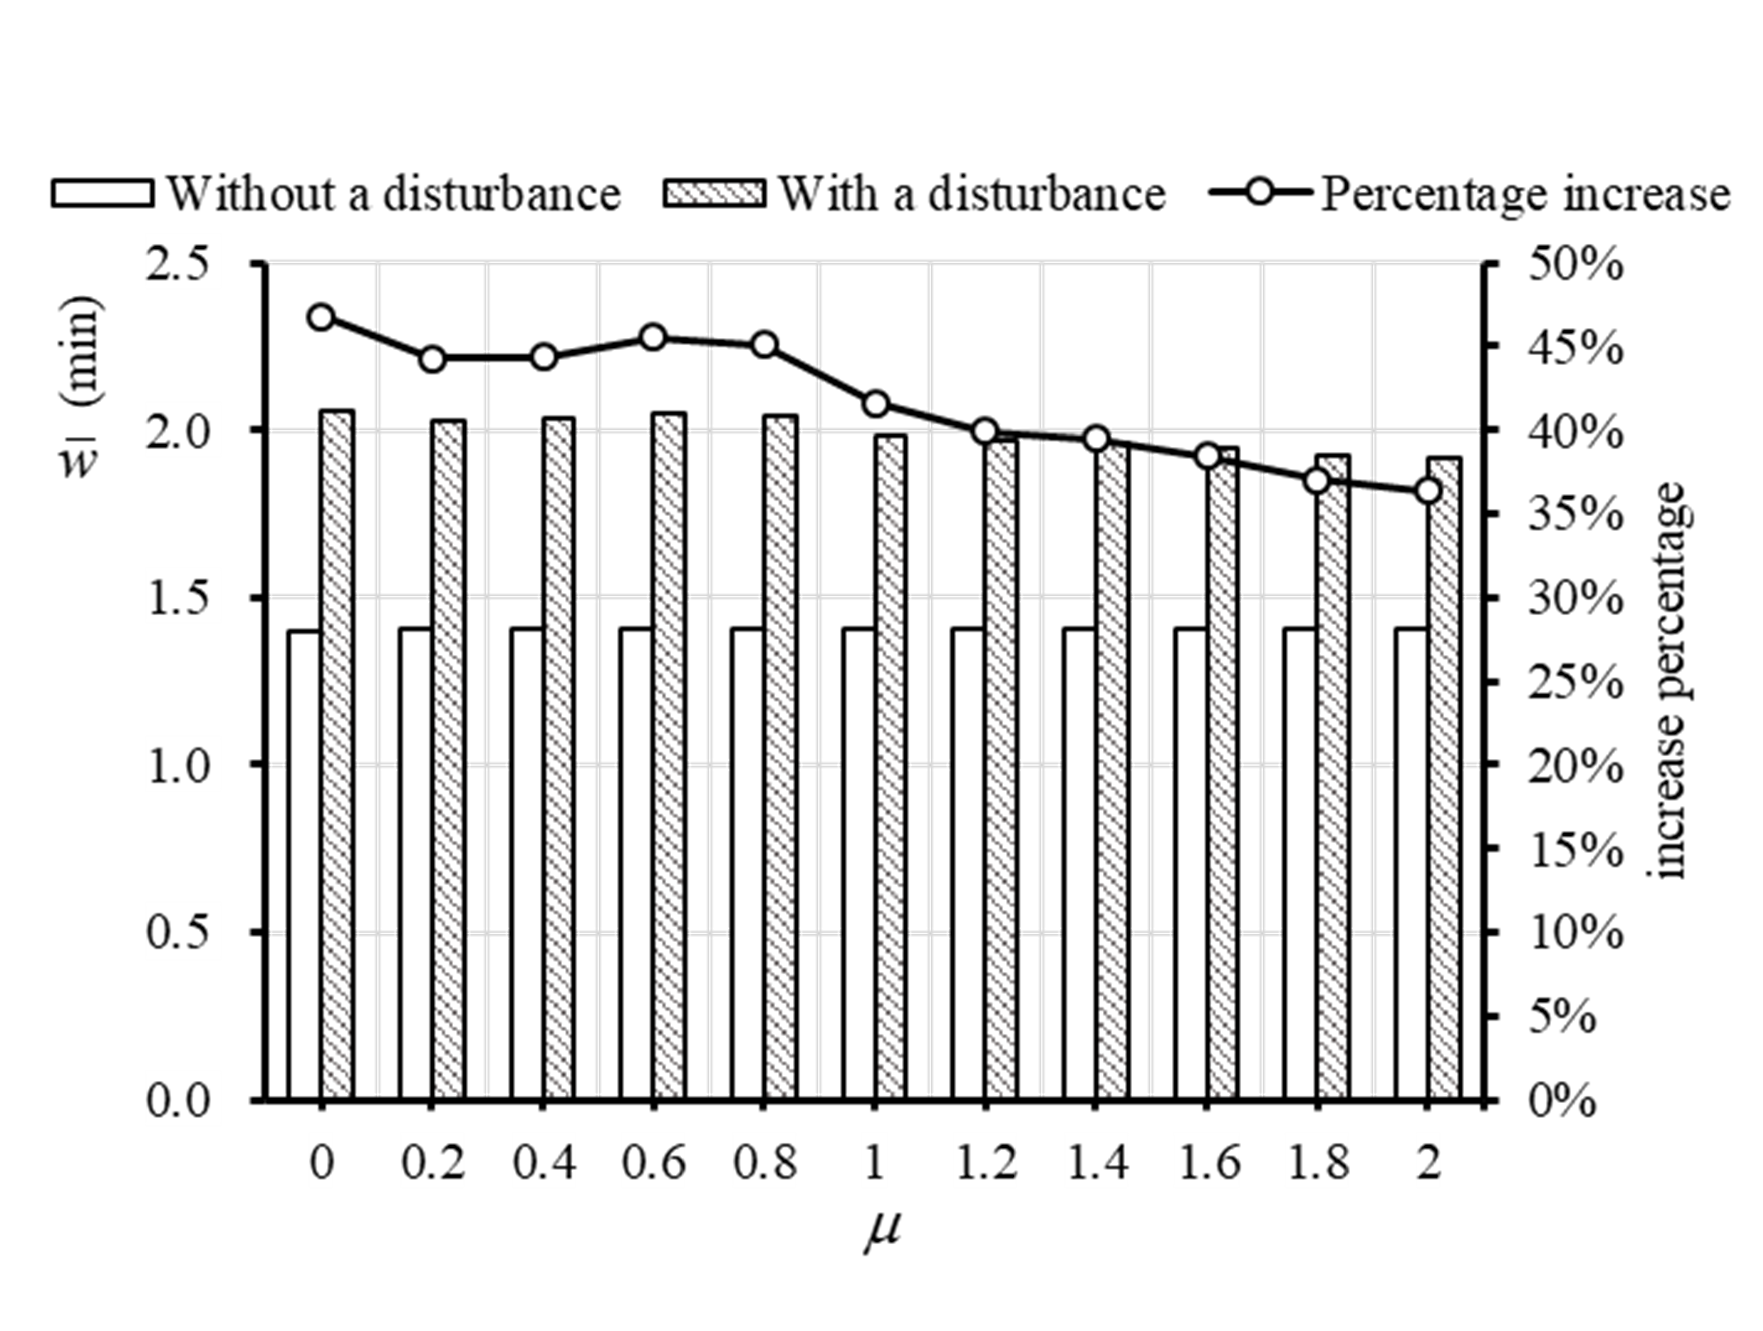
\includegraphics[width=0.45\textwidth]{CASPT2021paper_fig/trans ana 1.png}}}\\ \hline
        \subfloat[Average waiting time of line 1]{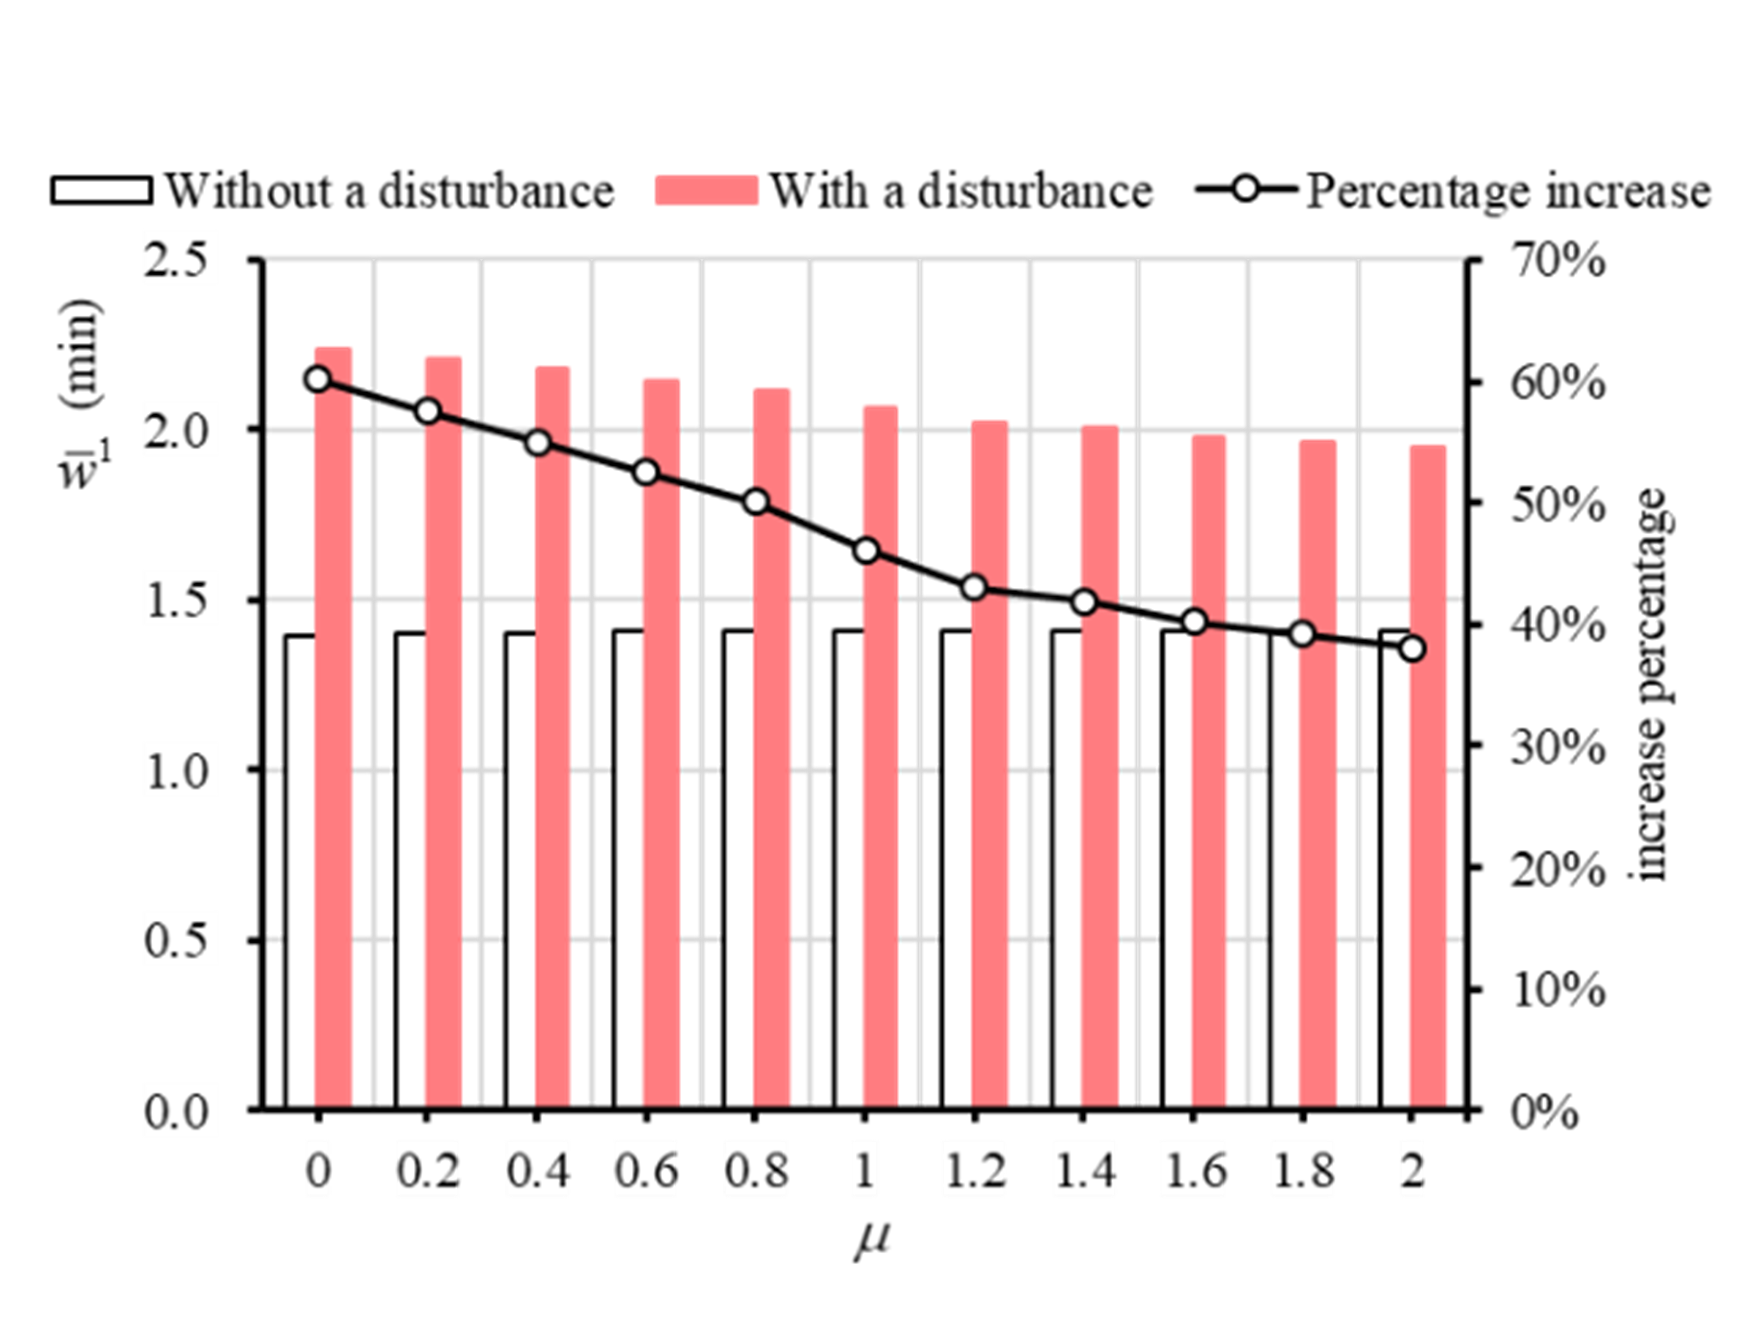
\includegraphics[width=0.45\textwidth]{CASPT2021paper_fig/trans ana 2.png}}
        &\subfloat[Average waiting time of line 2]{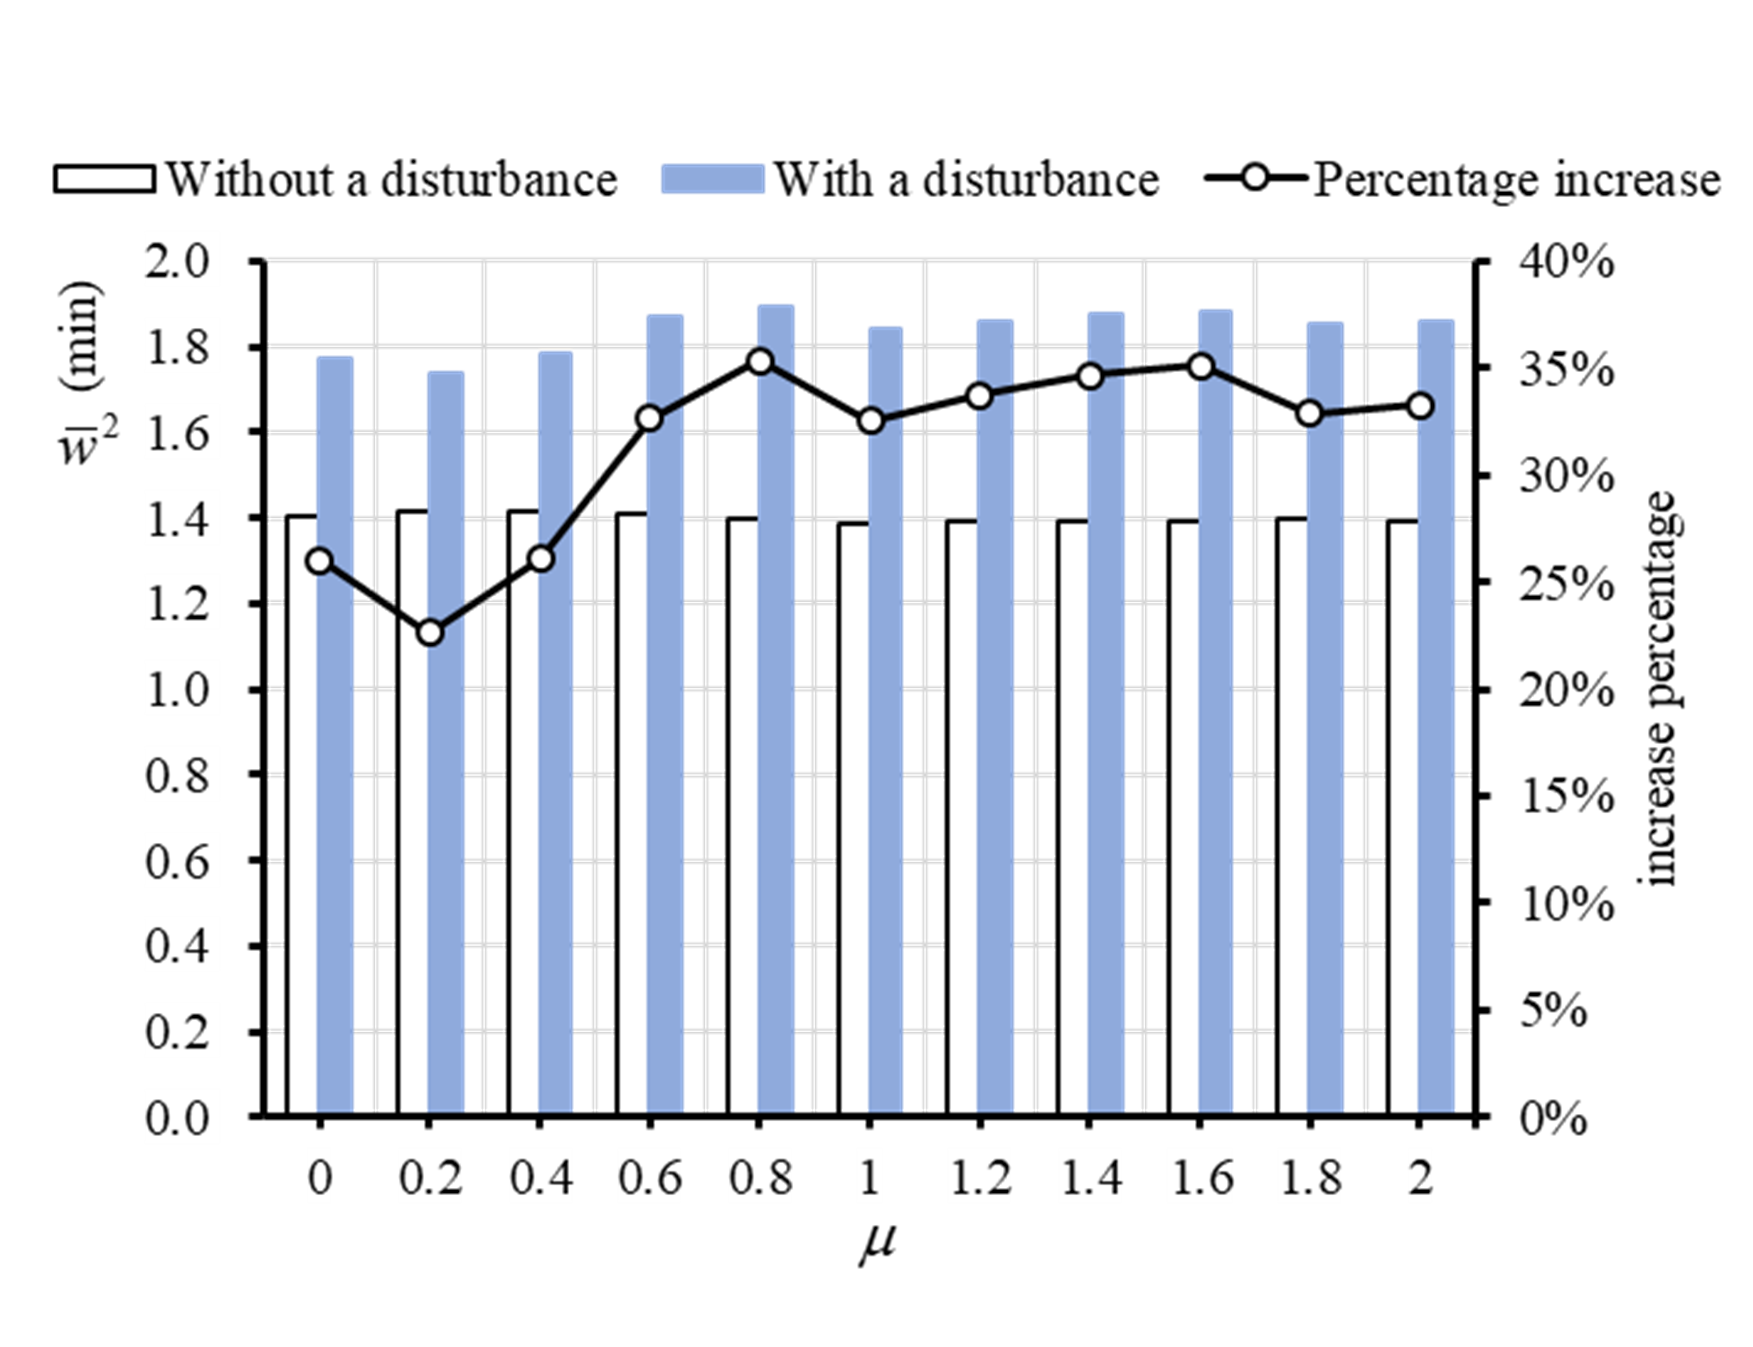
\includegraphics[width=0.45\textwidth]{CASPT2021paper_fig/trans ana 3.png}}\\ \hline
        \subfloat[STD of headway of line 1]{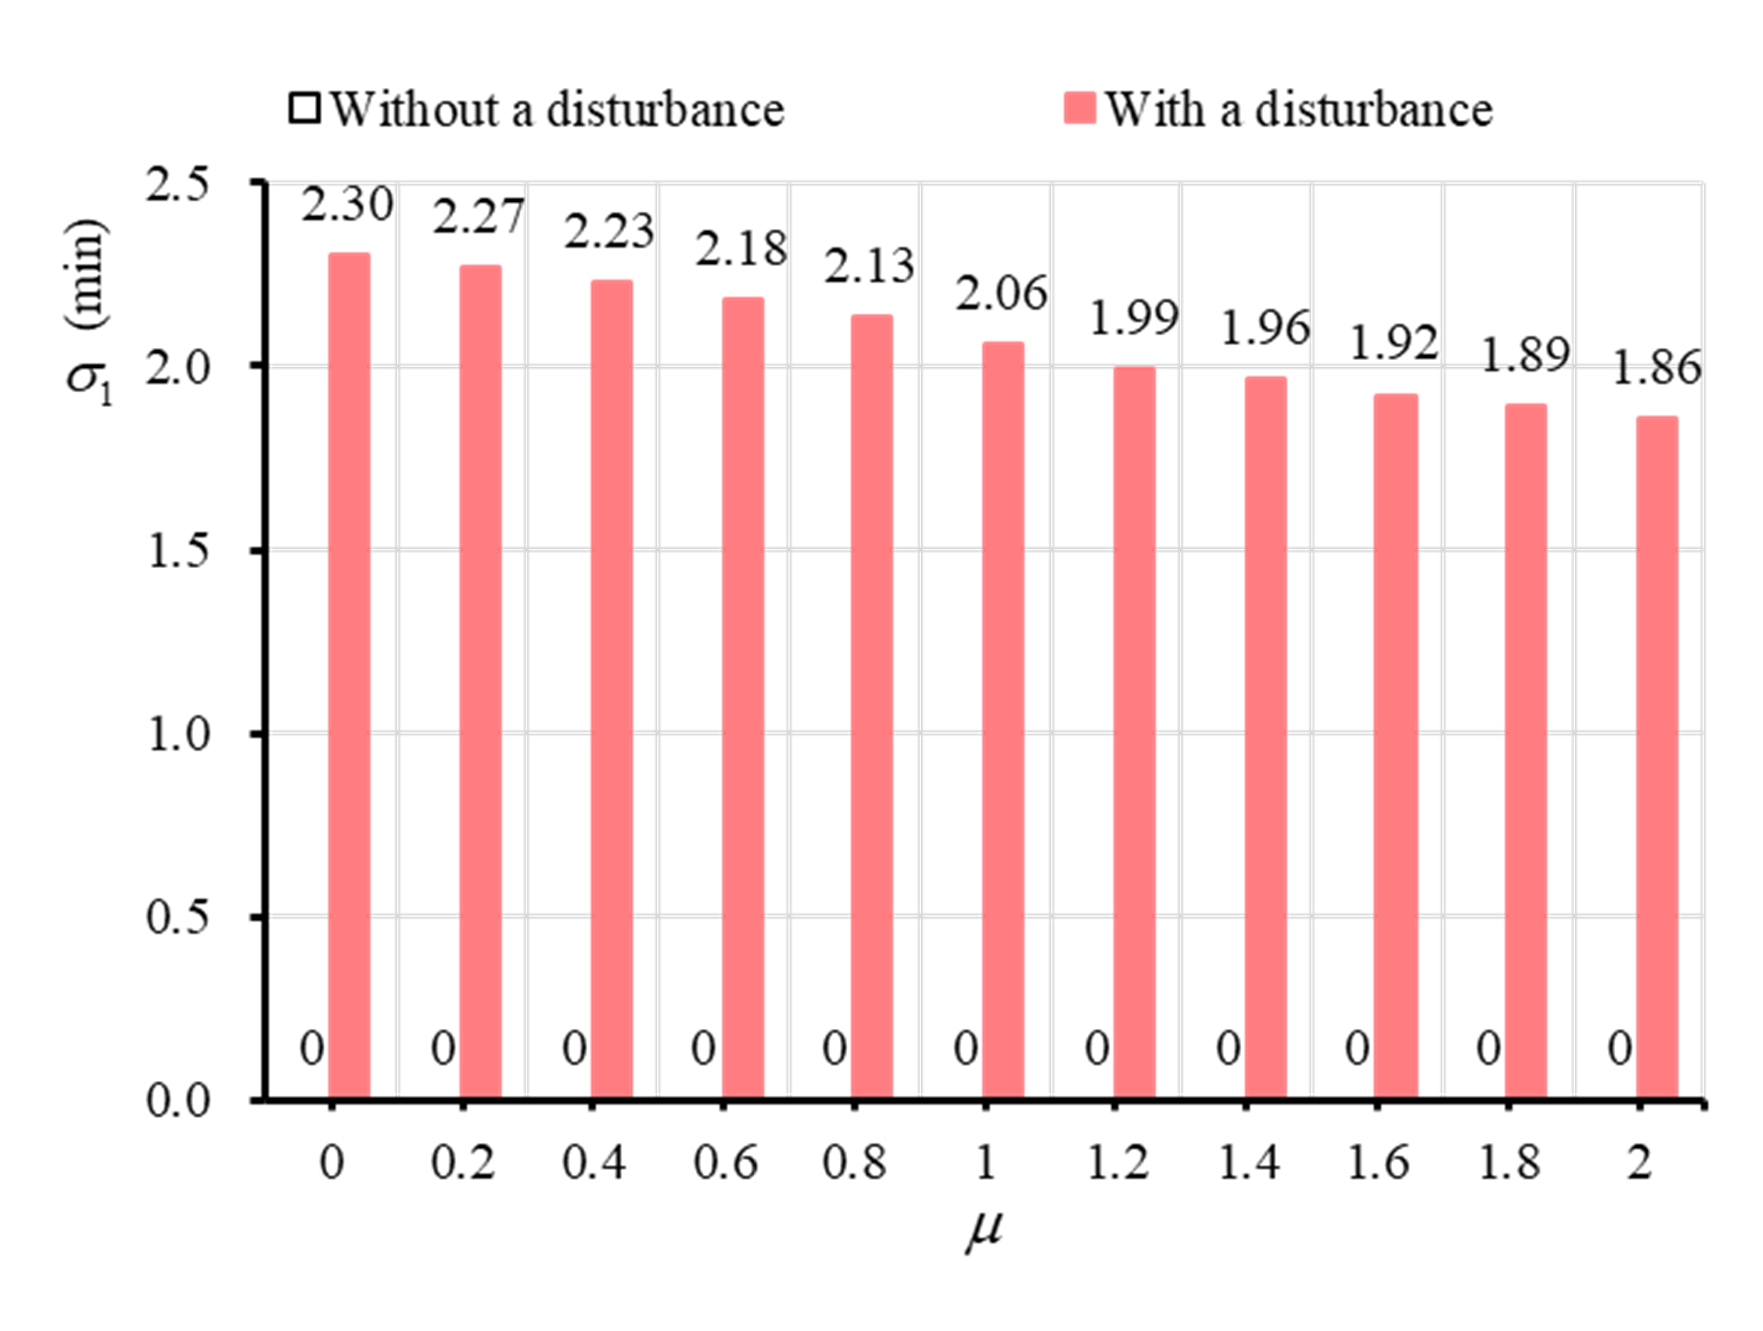
\includegraphics[width=0.45\textwidth]{CASPT2021paper_fig/trans ana 4.png}}
        &\subfloat[STD of headway of line 2]{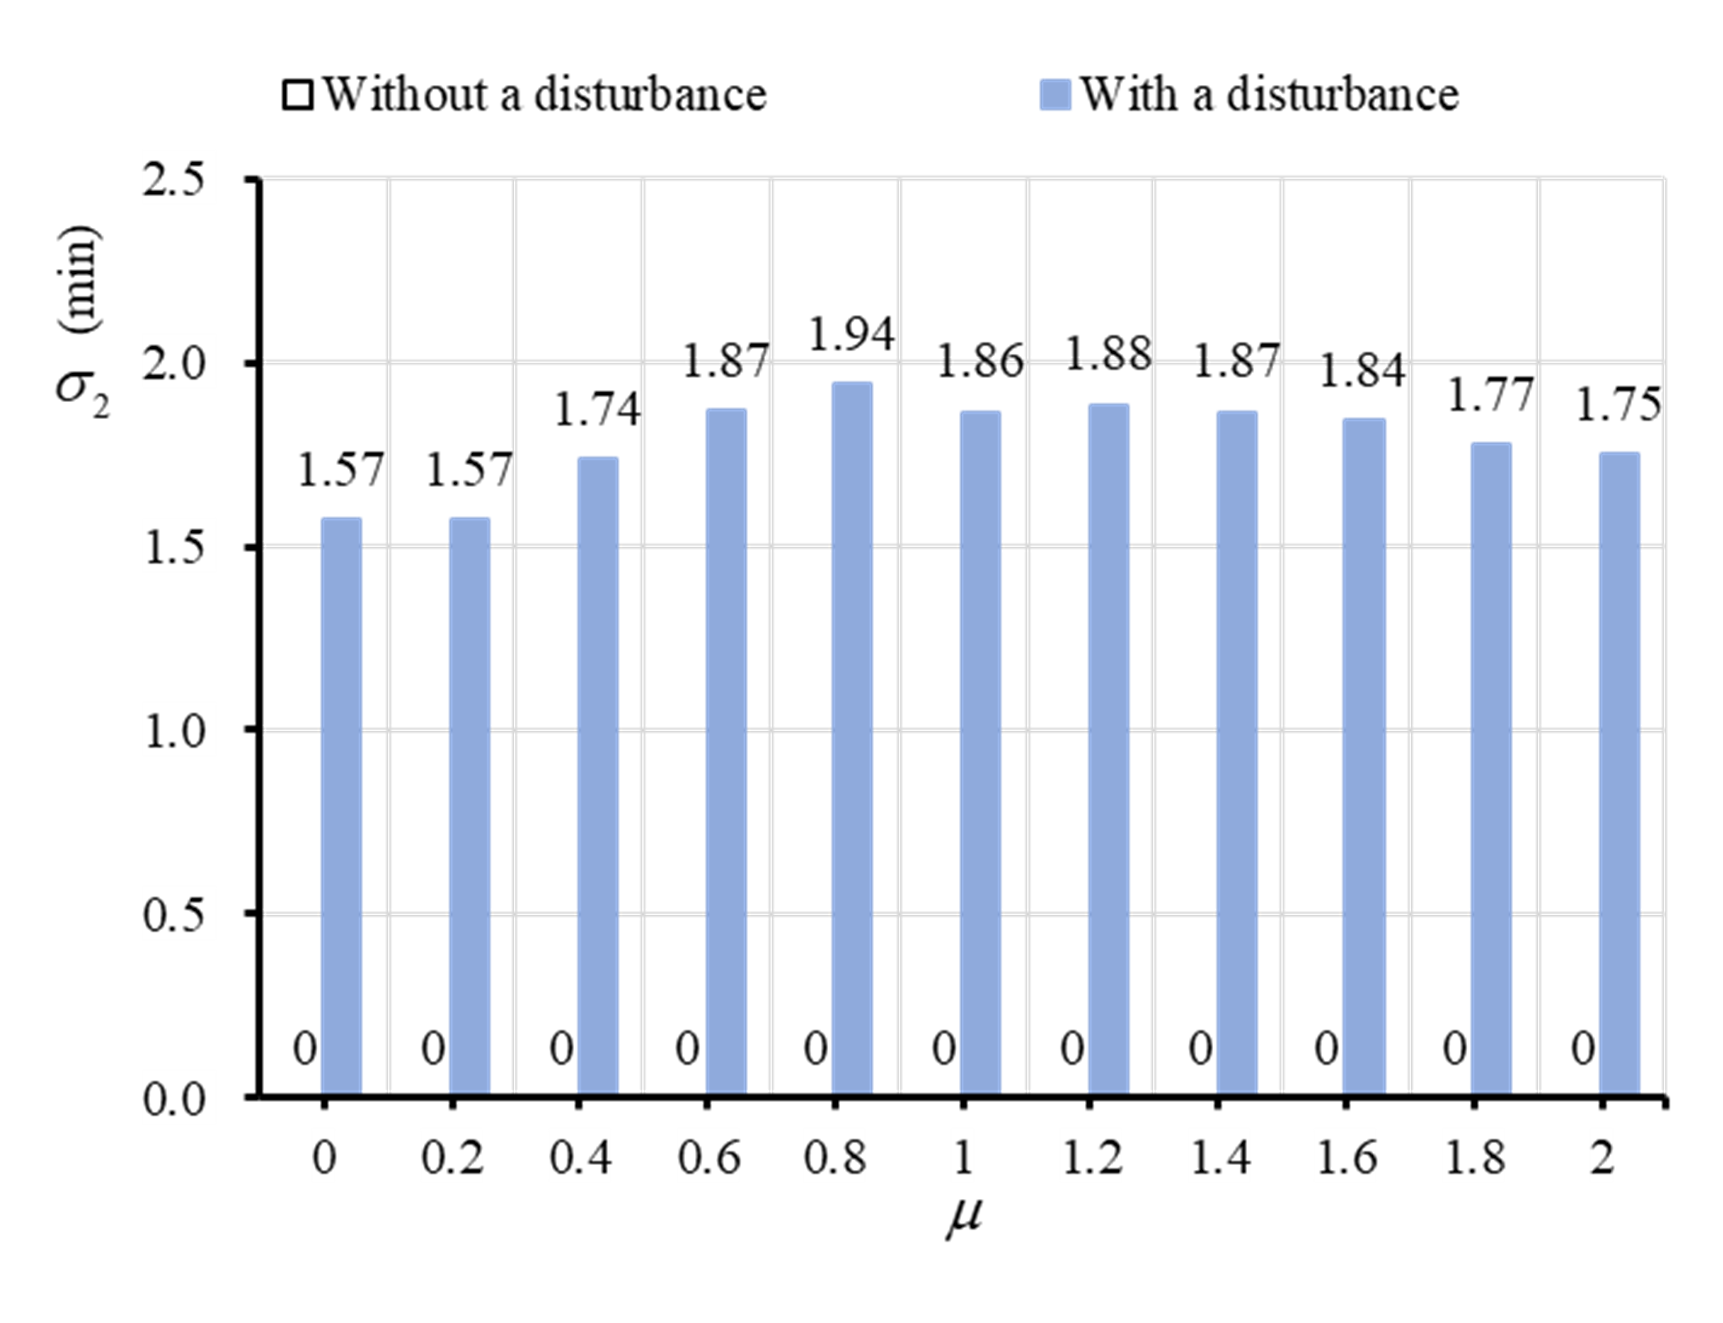
\includegraphics[width=0.45\textwidth]{CASPT2021paper_fig/trans ana 5.png}}         \\ \hline
        \end{tabular}
        \caption{The sensitivity analysis of transfer parameter}
        \label{fig:trans ana}
    \end{figure}

\subsubsection{Sensitivity to bus capacity}
In this analysis, the bus capacity is set from 120, 140 up to 200 (pas) while other parameters follow the basic settings in Table \ref{tab: basic settings}.
According to the results shown in Fig.\ref{fig:cap ana}, all evaluation indices remain stable when bus capacity changes in the condition without a disturbance.
It demonstrates that capacity constraint does not work as all buses are not full-loaded. 
In the condition with a disturbance, indicators with different bus capacity settings increase. 
What's more, the increases of average waiting time and standard deviation of headway are larger when bus capacity setting is larger.
The trend indicates that:
\begin{enumerate}[1)]
    \item Capacity constraint works when bus bunching occurs. In other words, there exist passengers failing to board because of the underutilization of the bunching buses.
    \item The impacts of bus bunching become more significant with the vehicle capacity increases, and the performance of the bus service tends to be worse.
\end{enumerate}

\begin{figure}[h]
  \centering
  \begin{tabular}{|c|c|}
      \multicolumn{2}{|c|}{\subfloat[Average waiting time of two lines]{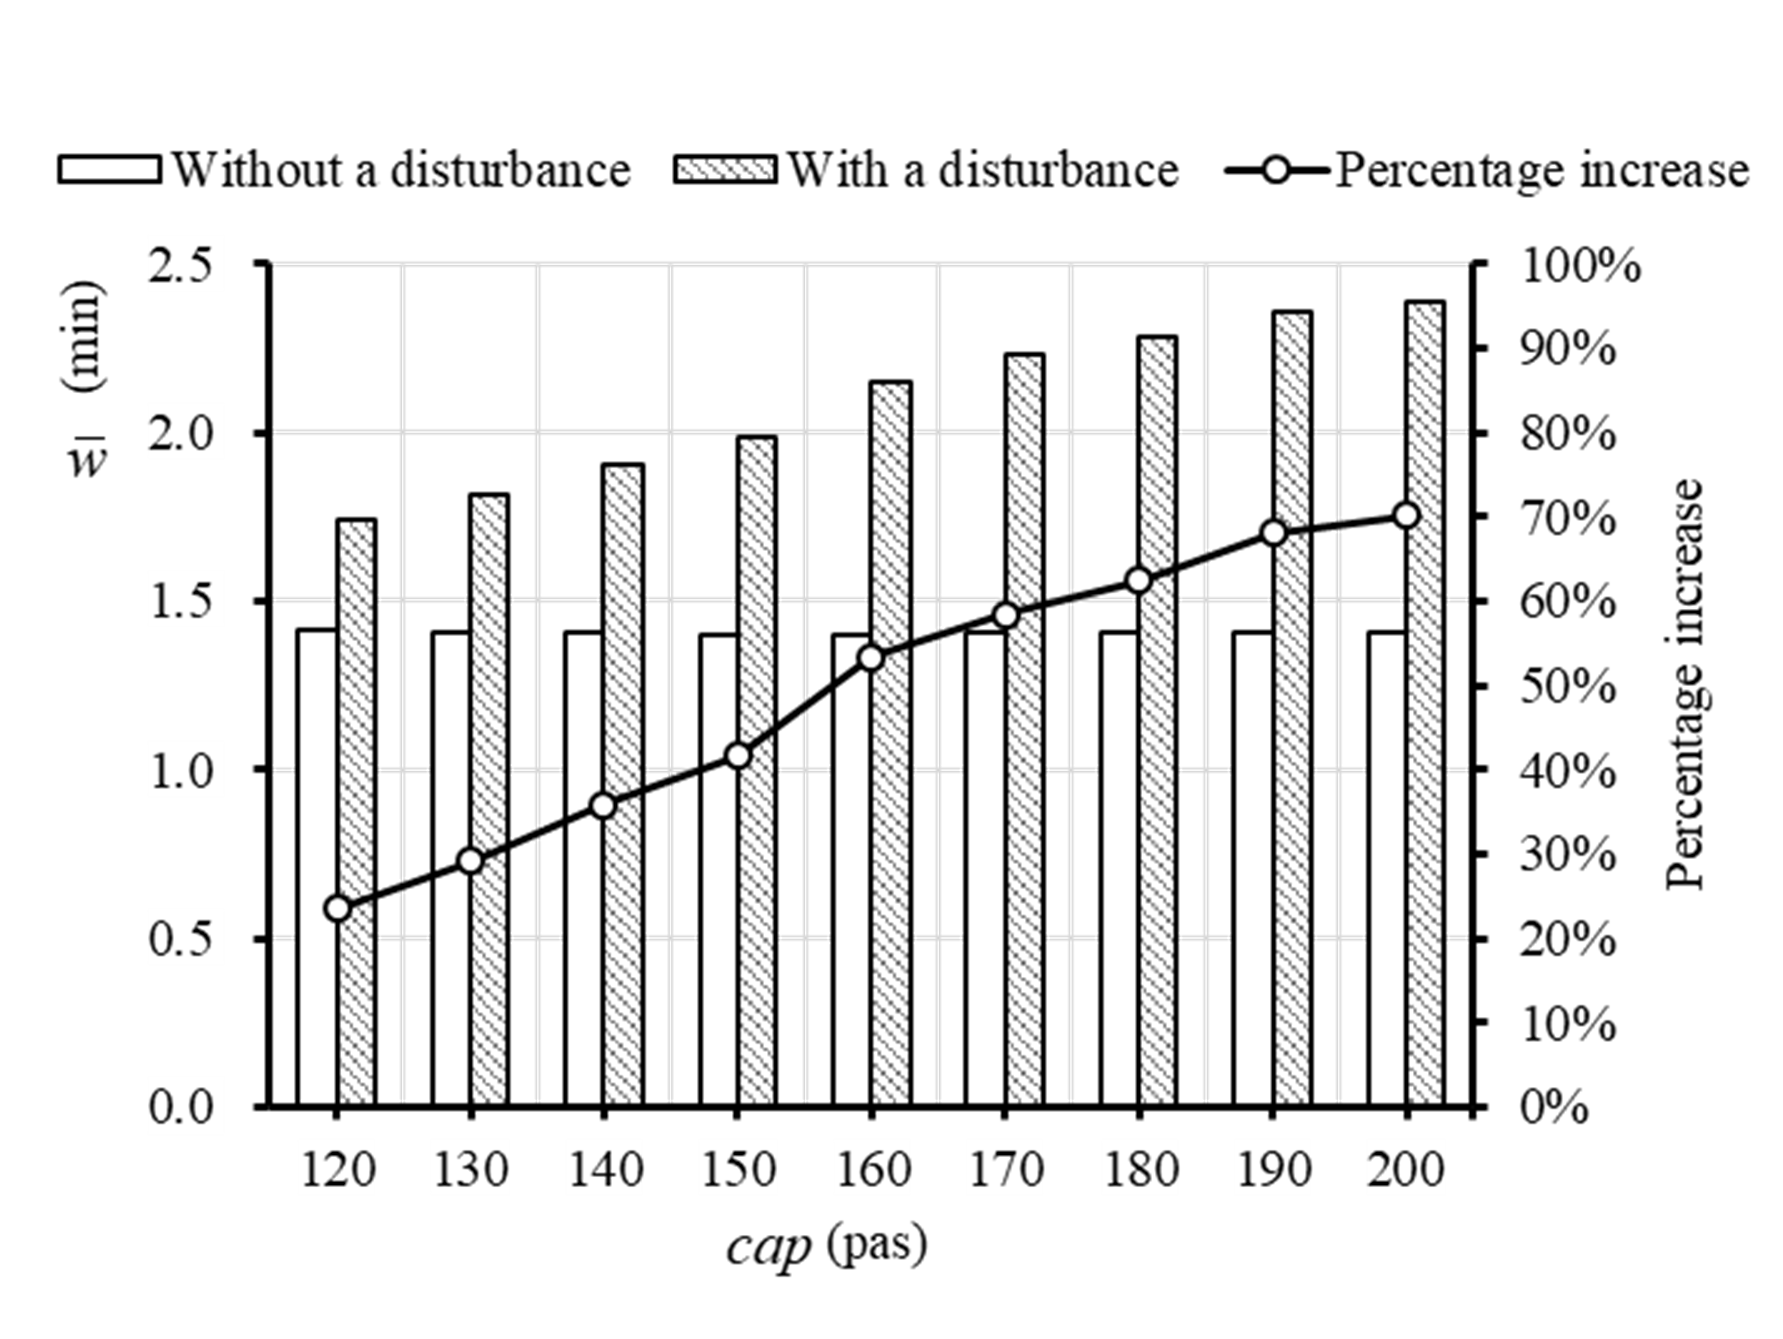
\includegraphics[width=0.45\textwidth]{CASPT2021paper_fig/cap ana 1.png}}}\\ \hline
      \subfloat[Average waiting time of line 1]{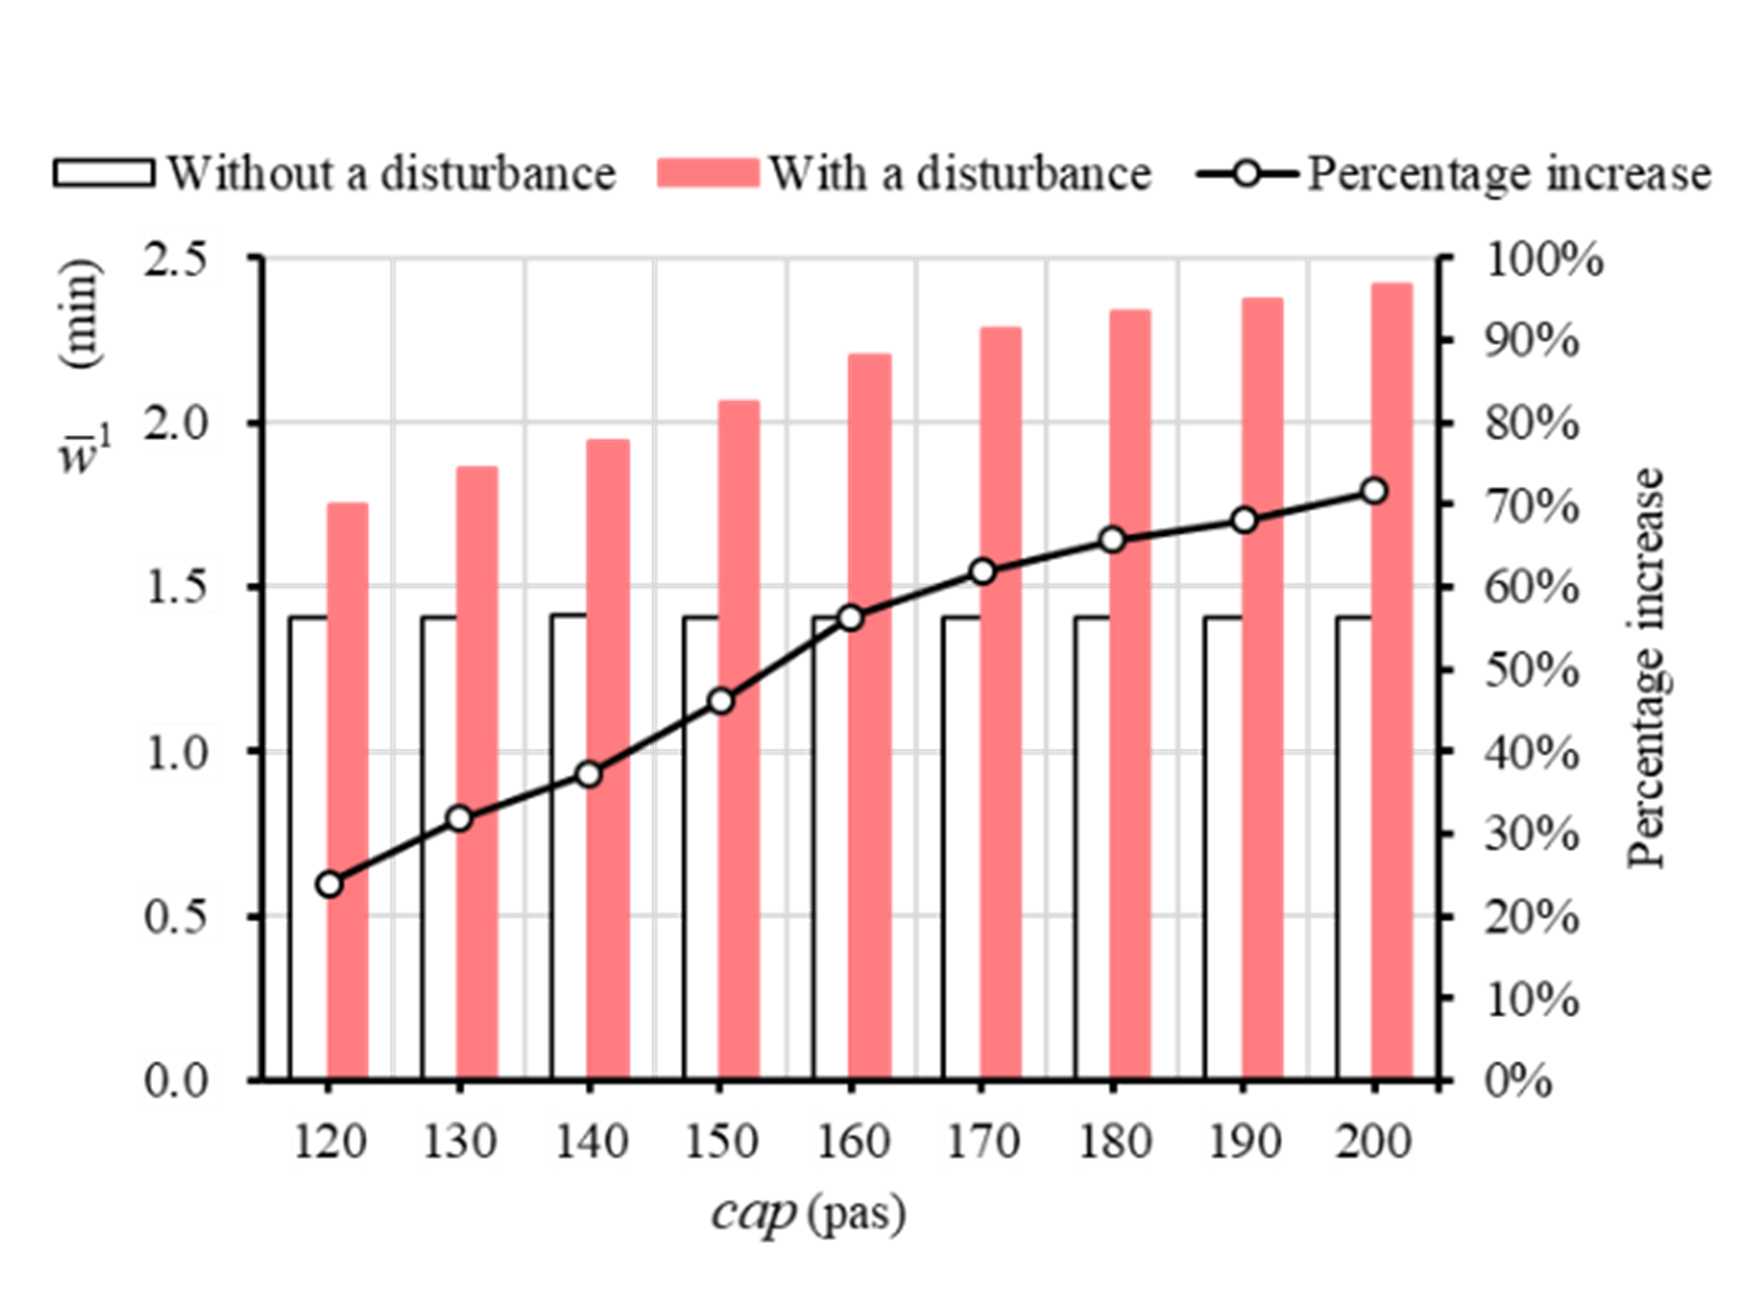
\includegraphics[width=0.45\textwidth]{CASPT2021paper_fig/cap ana 2.png}}
      &\subfloat[Average waiting time of line 2]{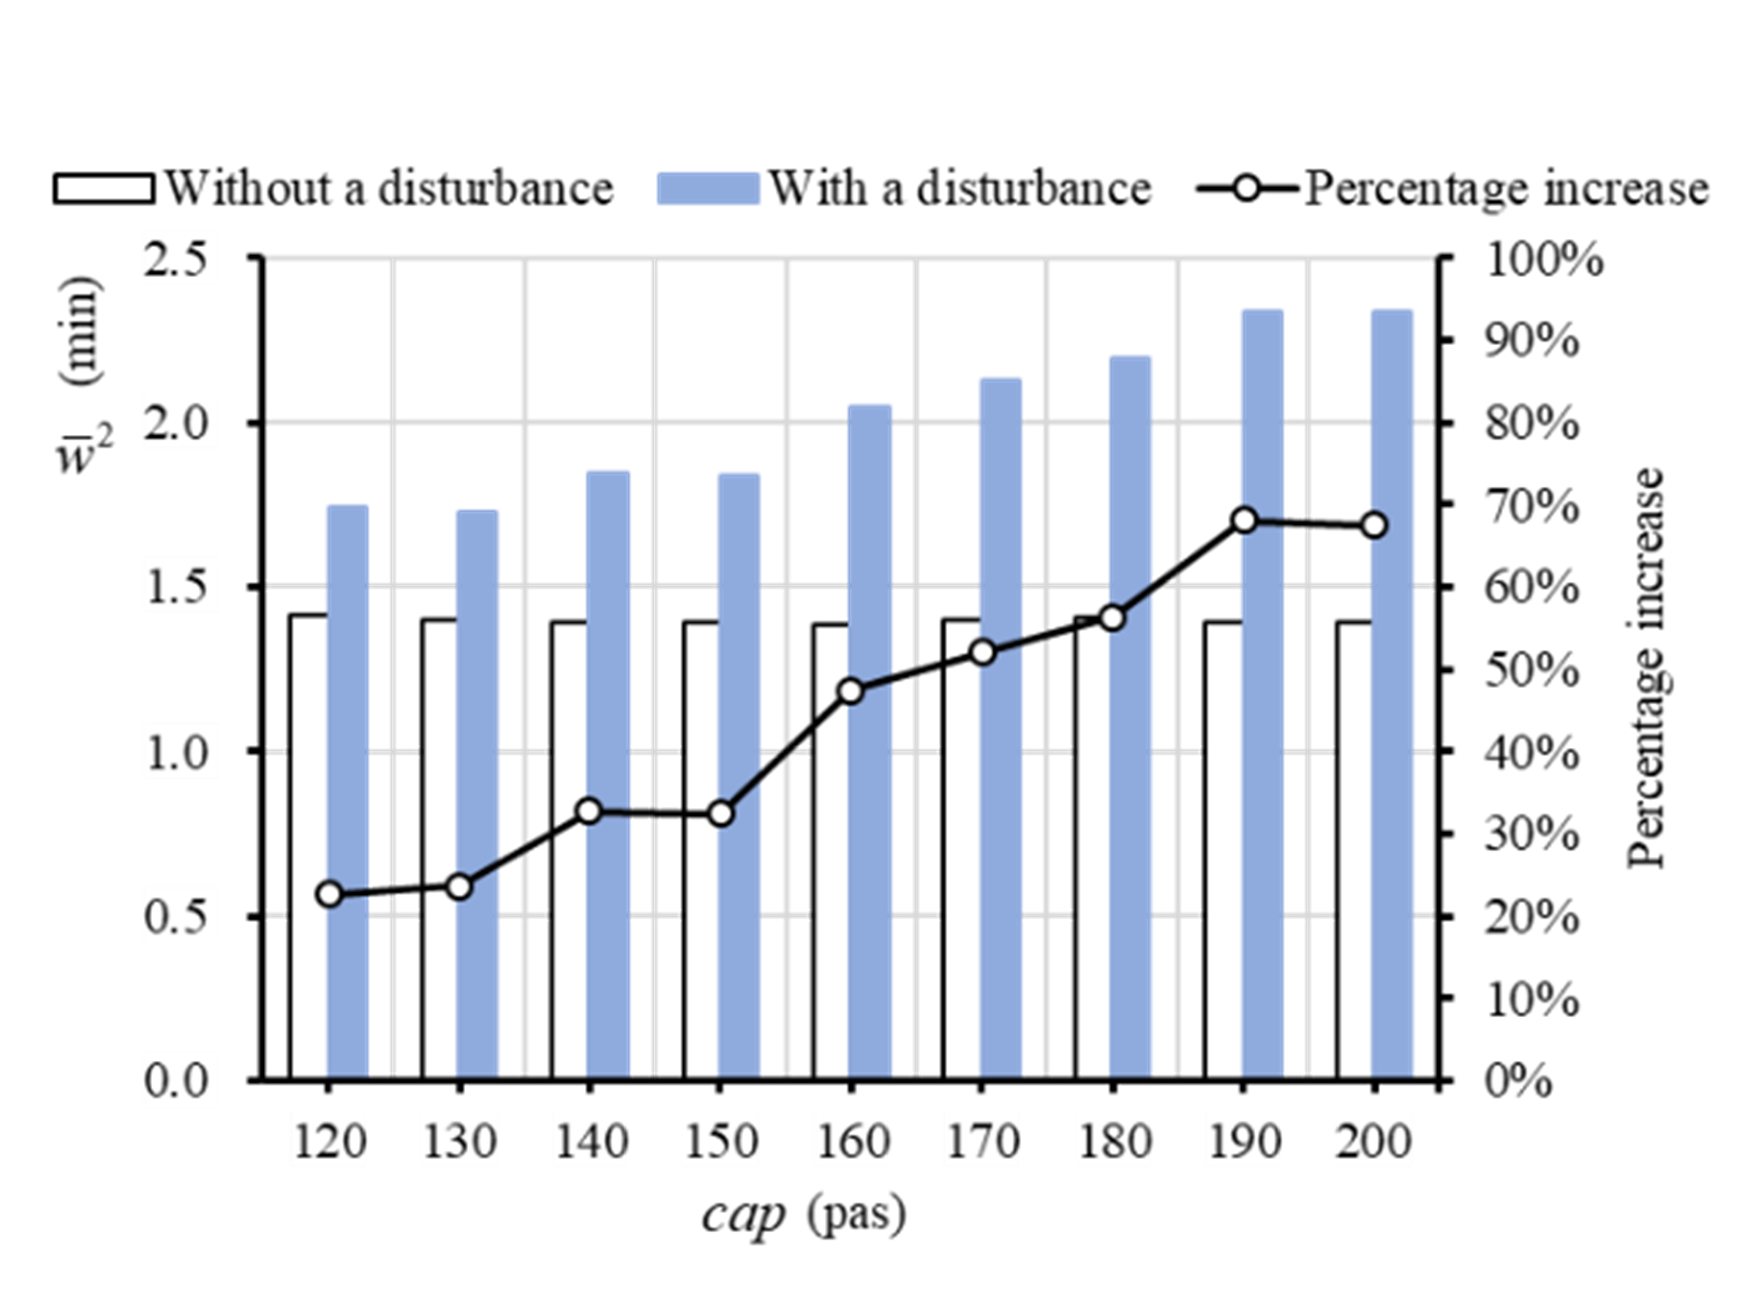
\includegraphics[width=0.45\textwidth]{CASPT2021paper_fig/cap ana 3.png}}\\ \hline
      \subfloat[STD of headway of line 1]{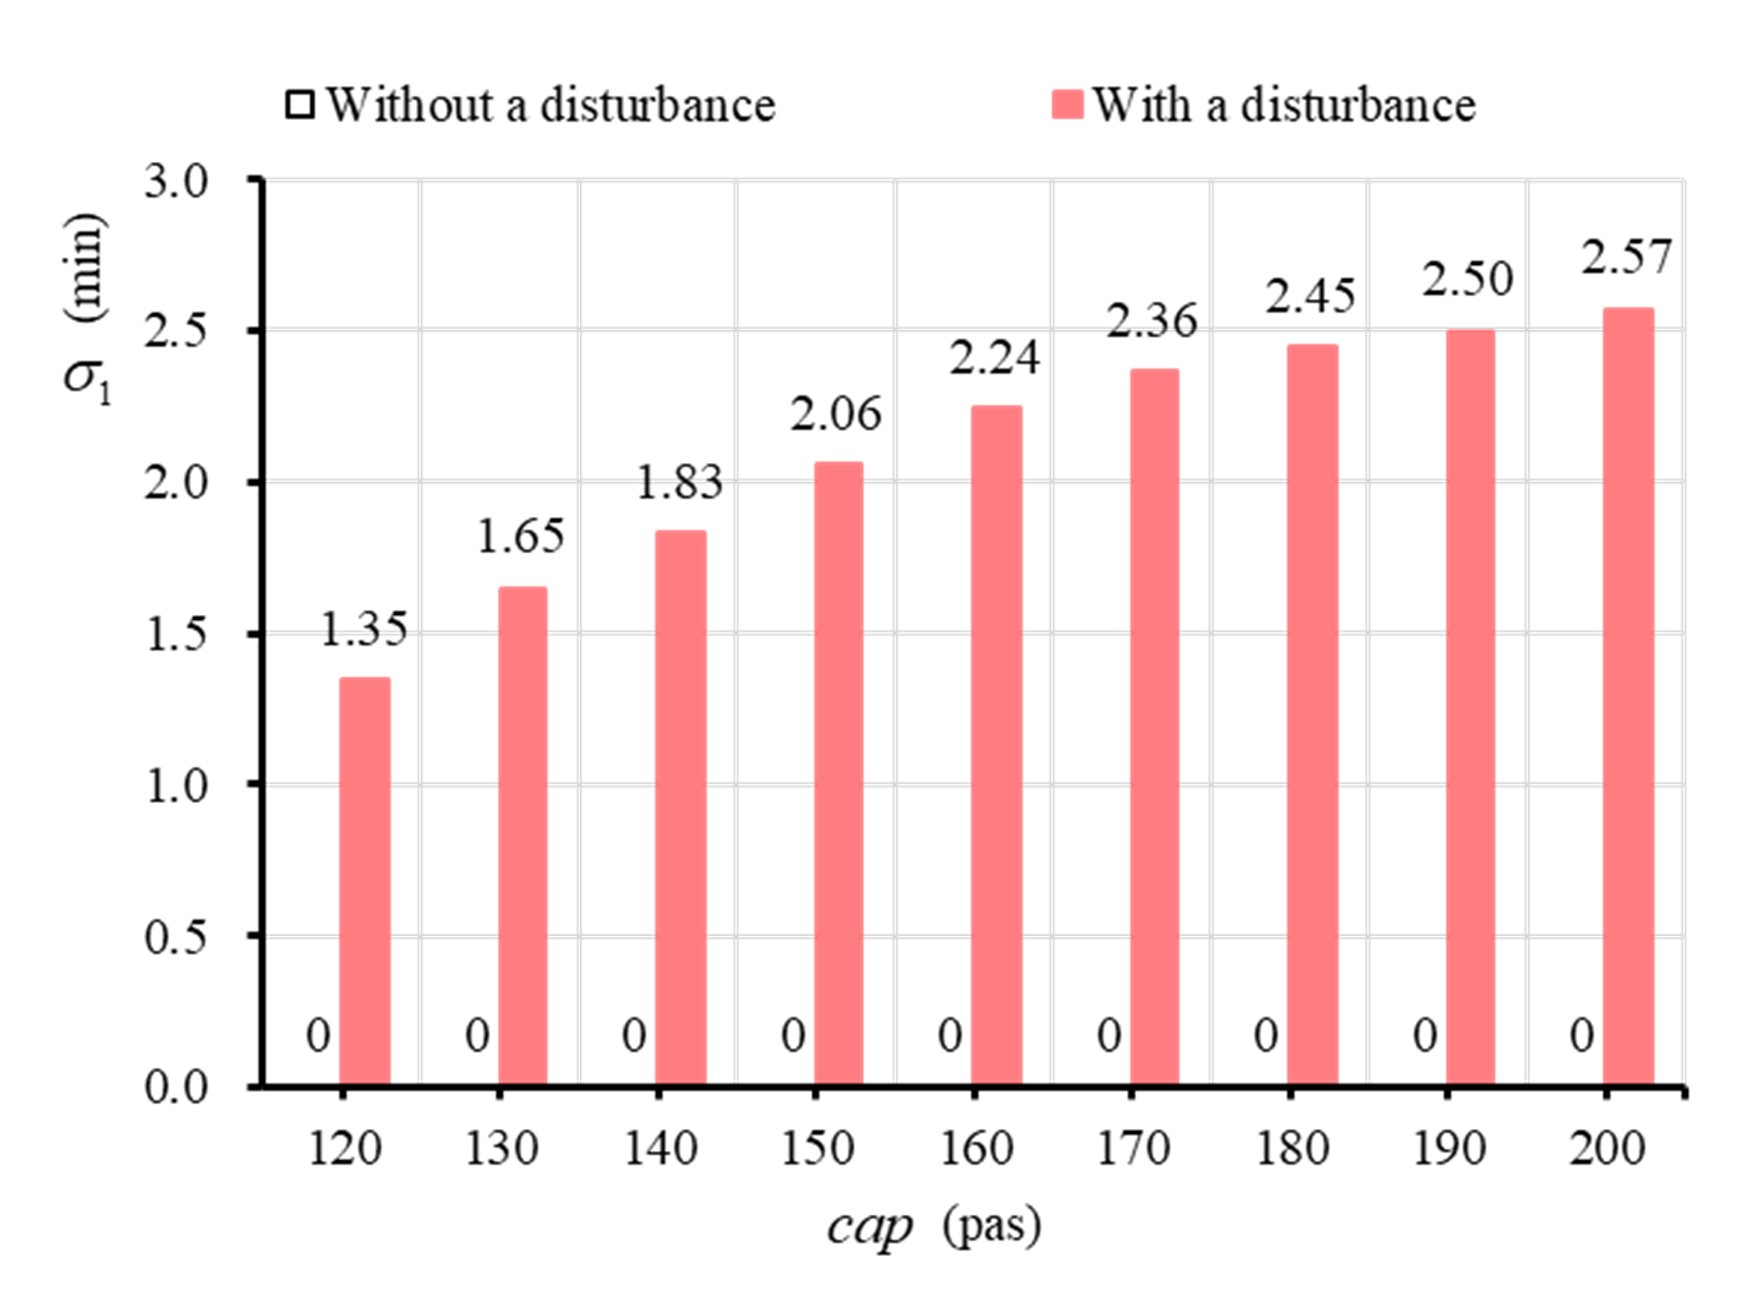
\includegraphics[width=0.45\textwidth]{CASPT2021paper_fig/cap ana 4.png}}
      &\subfloat[STD of headway of line 2]{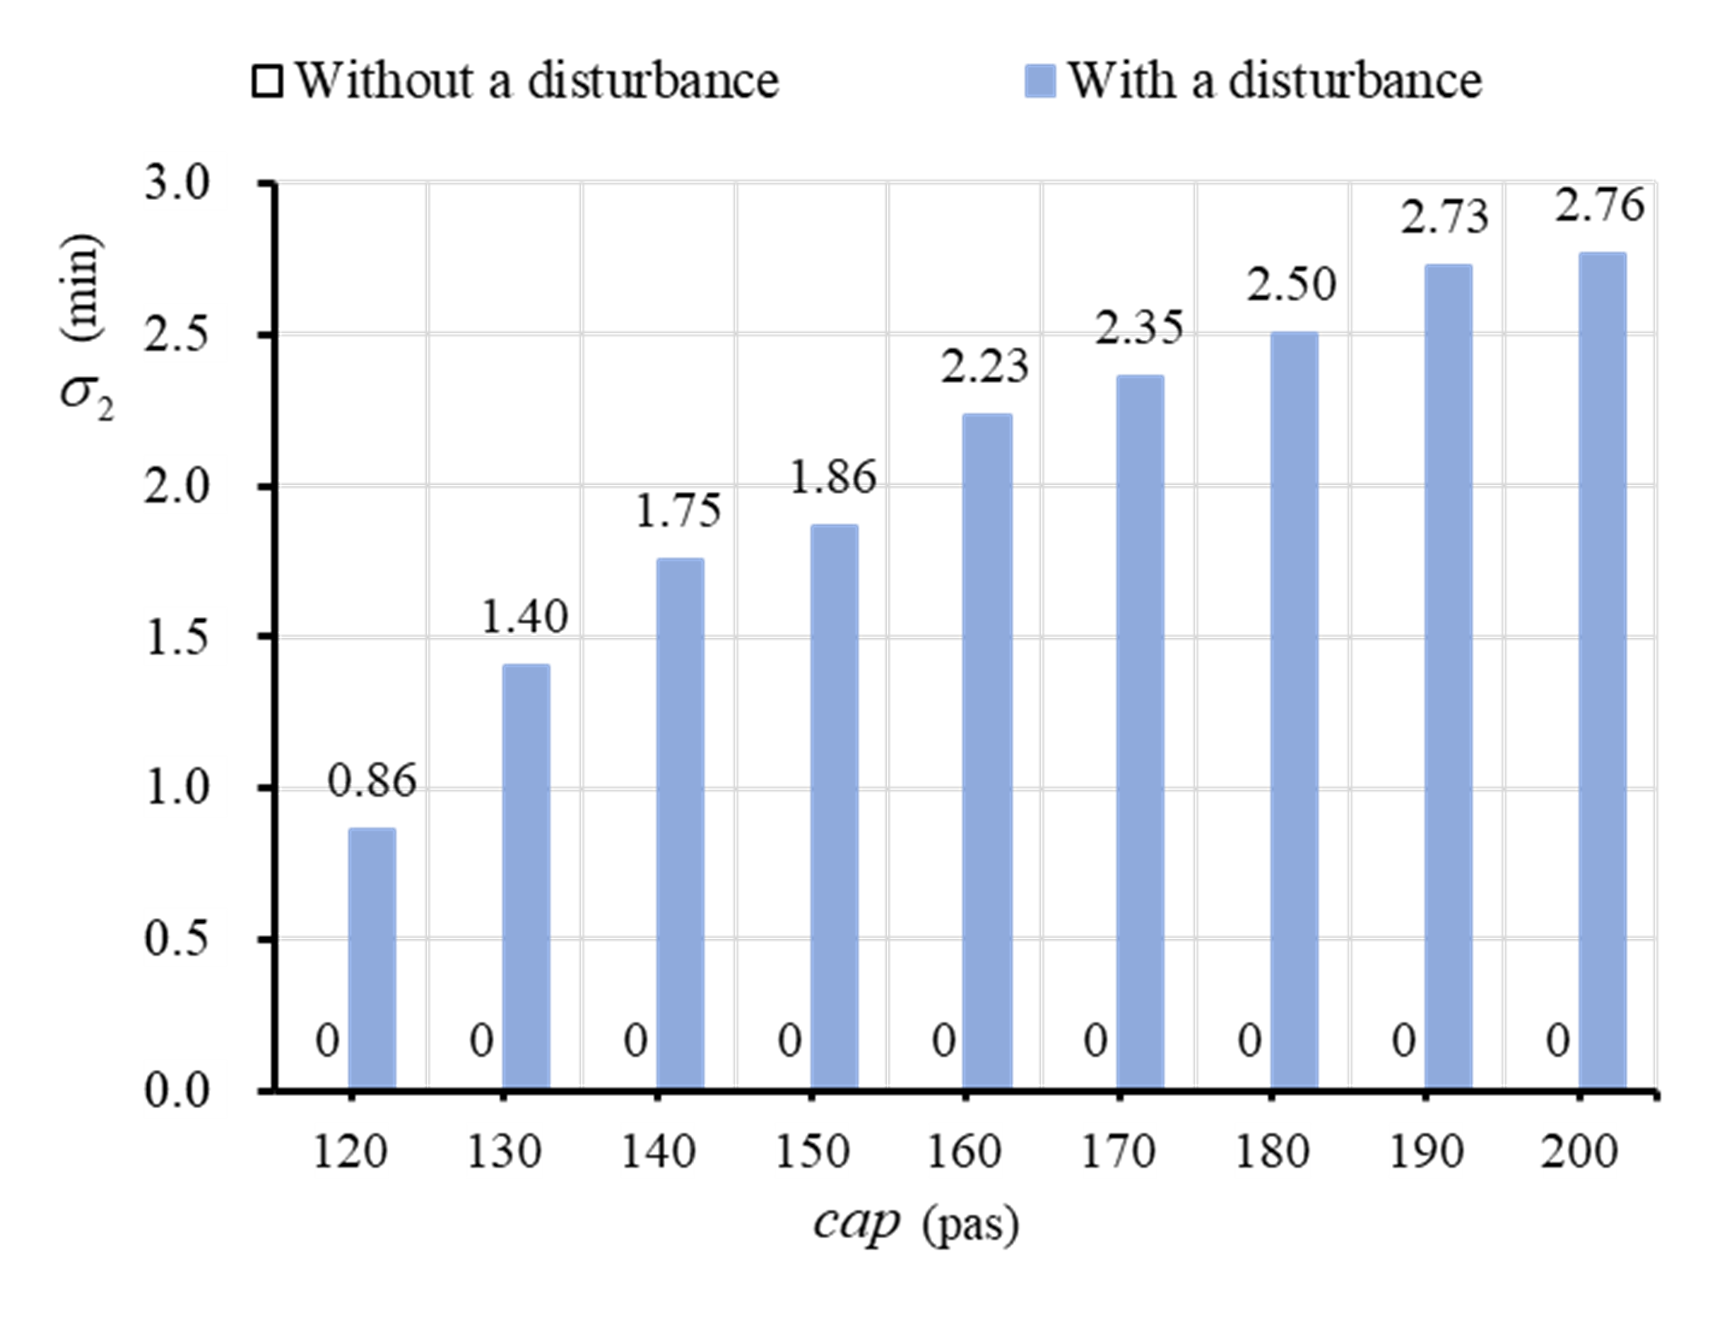
\includegraphics[width=0.45\textwidth]{CASPT2021paper_fig/cap ana 5.png}}   \\ \hline      
      \end{tabular}
      \caption{The sensitivity analysis of bus capacity}
      \label{fig:cap ana}
  \end{figure}

\section{Conclusions}\label{conclusions}
This study develops a methodology for investigating the bus bunching phenomenon.
Compared with existing models, the advance of the proposed method is that the capacity constraint and passengers transfer behavior are simultaneously considered in a multi-lane scenario. 
Meanwhile, the algorithm for obtaining bus trajectories and passengers' transfer flow are developed. 
Case studies were carried out to examine the effects of capacity constraint and passengers transfer behavior on the propagation of bus bunching.
\textcolor{red}{performance indicator}
Moreover, three performance indicators, namely, xxxx, are proposed to measure the sensitivity of different parameters on the impacts of the bus bunching.
\textcolor{red}{enhance?}
Notably, the results of the experiments show that increasing the transfer passenger flow enhance the propagation of bus bunching phenomenon from a disturbed line to an undisturbed line, implying that motivating passenger behaviors (demand side) have the potential to cooperate with operation tactics (supply side) to alleviate the bus bunching problem.

\textcolor{red}{todo, 
future research direction, why they are important or neccessary 
elaborate more, justify, literature, 
also add discussion relate the equilibrium behaviors
}
This study opens many research directions, including but not limited to: 
\begin{enumerate}[1)]
    \item Examining the effect of different combinations of bus service frequencies and offsets; 
    \item Generalizing the modeling framework for a transit corridor served by more than two transit lines; 
    \item Relaxing the assumptions of the proposed model. 
    For example, allowing more than one platform for different bus lines to board and alight passengers at some larger transfer stops; 
    \item Develop a simulation-based optimization framework to optimize the control strategy (e.g. bus holding) considering common line issues and passenger equilibrium behaviors.
\end{enumerate}

% %%%%%%%%%%%%%%%%%%%%%%%%%%%%%%%%%%%%%%%%%%%%%%%%%%%%%%%%%%%%%%%%%%%%%%%%%%%%%%%%%%%%%%
% %%%%%%%%%%%%%%%%%%%%%%%%%%%%%%%%%%%%%%%%%%%%%%%%%%%%%%%%%%%%%%%%%%%%%%%%%%%%%%%%%%%%%%
% %%%%%%%%%%%%%%%%%%%%%%%%%%%%%%%%%%%%%%%%%%%%%%%%%%%%%%%%%%%%%%%%%%%%%%%%%%%%%%%%%%%%%%
% %\begin{acknowledgements}
% %If you'd like to thank anyone, place your comments here
% %and remove the percent signs.
% %\end{acknowledgements}

\section*{Appendix: Proof of proposition 1}
\appendix
Without loss of generality, we assume bus $m$ is the following bus of line $r$ that arrives at the first common stop $n_{1}$ after its preceding bus of line $r'$ denoted as $m^{r'}(m,n_{1})$.
% (i.e. $\frac{\bar{B}_{m,n}}{B_{m,n}}=1,\forall m\in \mathcal{M}^{1}\cup \mathcal{M}^{2};n\in S^{1}\cup S^{2}$), 
As all buses are not full-loaded, the transfer cost function via common stop $n_{i}$ to line $r$ for transfer passengers on bus $m^{r'}\left(m,n_{1}\right)$ 
degenerates to the headway between bus $m^{r'}\left(m,n_{1}\right)$ and bus $m$.
\begin{equation}
    \omega_{n_i}^{m^{r'}\left(m,n_{1}\right)} = \omega_{n_i}^{m^{r'}\left(m,n_{1}\right),m} 
    = d_{m,n_{i}}-d_{m^{r'}\left(m,n_{1}\right),n_{i}}
    \end{equation}


The depart time of bus $m$ from stop $n_{i}$ is calculated by:
\begin{equation}
    \label{equ:d_com}
    d_{m,n_{i}} = 
    \begin{cases}
        a_{m,n_{1}} + \sum\limits_{k=1}^{i} W_{m,n_{k}} + \sum\limits_{k=1}^{i-1} T_{m,n_{k}} &\text{ if } i=2,...,\left|\mathcal{N}_{com}^{r,r'}\right|\\
        a_{m,n_{1}}+W_{m,n_{1}} &\text{ if } i=1
    \end{cases}
\end{equation}
Therefore, the transfer cost function from bus $m$ to line $r'$ is expressed by:
\begin{equation}
    \omega_{n_i}^{m^{r'}\left(m,n_{1}\right)}=  
    \begin{cases}
        a_{m,n_{1}} + \sum\limits_{k=1}^{i} W_{m,n_{k}} + \sum\limits_{k=1}^{i-1} T_{m,n_{k}}-d_{m^{r'}\left(m,n_{1}\right),n_{i}}
        &\text{ if }i=2,...,\left|\mathcal{N}_{com}^{r,r'}\right|\\
        a_{m,n_{1}} + W_{m,n_{1}}-d_{m^{r'}\left(m,n_{1}\right),n_{i}}
        &\text{ if }i=1.
    \end{cases}
\end{equation}    
The dwell time of bus $m$ at common stop $n_{i}\in\mathcal{N}_{com}^{r,r'}$ is derived by:
\begin{equation}
    \label{equ:W_com}
    \begin{split}
        W_{m,n_{i}} &= \max \left\{W_{m,n_{i}}^{A},\min \left\{W_{m,n_{i}}^{B},\frac{C_{m,n_{i}}}{\beta}\right\}\right\}\\
        & = \max \left\{W_{m,n_{i}}^{A},W_{m,n_{i}}^{B} \right\}\\
        & = \max \left\{\frac{A_{m,n_{i}}}{\alpha},W_{m,n_{i}}^{B} \right\}\\
    \end{split}
\end{equation}
where % $L_{m^{r,r'}(m,n_{i}),n_{i}}^{r,r'}=0$
\begin{equation}
    \begin{split}
        W_{m,n_{i}}^{B} &= \frac{\left(a_{m,n_{i}}-d_{m^{r,r'}(m,n_{i}),n_{i}}\right)\cdot \left(\Lambda_{n_{i}}^{r}+\Lambda_{n_{i}}^{r,r'}\right)
        +L_{m^{r,r'}(m,n_{i}),n_{i}}^{r}}
        {\beta-\left(\Lambda_{n_{i}}^{r}+\Lambda_{n_{i}}^{r,r'}\right)}\\
        &= \frac{\Lambda_{n_{i+1}}^{r,r'}\cdot I_{m,n_{i+1}}^{r,r'} + \Lambda_{n_{i+1}}^{r}\cdot I_{m,n_{i+1}}^{r} + 
        \sum\limits^{m'\in\mathcal{M'}(m-1,m)} P_{m'}^{trans}\cdot\alpha_{m',n_{i+1}}}
        {\beta-\left(\Lambda_{n_{i}}^{r}+\Lambda_{n_{i}}^{r,r'}\right)}
    \end{split}
\end{equation}
and
\begin{equation}
    A_{m,n_{i}} = p_{m,n_{i},n_{i}} + \alpha_{m,n_{i}}\cdot P_{m}^{trans}
\end{equation}
where $P_{m}^{trans}=\sum\limits_{j\in\mathcal{N}_{down}^{r'}} p_{m,n_{1},j}$ denotes the total number of transfer passengers on bus $m$.

Denote $\mathcal{M'}(m-1,m) = \{m'|d_{m-1,n_{i+1}}<d_{m',n_{i+1}}<d_{m,n_{i}},m'\in\mathcal{M}^{r'}\}$, and we get:
\begin{equation}
    \begin{split}
        W_{m,n_{i+1}} &= \max \left\{\frac{A_{m,n_{i+1}}}{\alpha},W_{m,n_{i+1}}^{B} \right\}\\
        &= \max \left\{W^{A}_{m,n_{i+1}}\left(\alpha_{m,n_{i+1}}\right),
        W_{m,n_{i+1}}^{B}(\overset{m'\in\mathcal{M'}(m-1,m)}{\left[\alpha_{m',n_{i+1}}\right]}) \right\}\\
        &=W_{m,n_{i+1}}\left(\alpha_{m,n_{i+1}},\overset{m'\in\mathcal{M'}(m-1,m)}{\left[\alpha_{m',n_{i+1}}\right]}\right)\\
    \end{split}
\end{equation}

The difference of cost function of two successive common stops are expressed as:
\begin{equation}
    \begin{split}
        &\omega_{n_{i+1}}^{m^{r'}\left(m,n_{1}\right)} - \omega_{n_{i}}^{m^{r'}\left(m,n_{1}\right)}\\
        &=W_{m,n_{i+1}} + T_{m,n_{i}} - \left(T_{m^{r'}(m,n_{1}),n_{i}} + W_{m^{r'}\left(m,n_{1}\right),n_{i+1}}\right) \\
        &=W_{m,n_{i+1}}-W_{m^{r'}\left(m,n_{1}\right),n_{i+1}}\\
    \end{split}
\end{equation}

If all common stops are used, the equilibrium conditions are equivalent to:
\begin{equation}
    \label{equ:equivalent condition}
    \begin{cases}
        \omega_{n_{i}}^{m'} - \omega_{n_{i-1}}^{m'} = 0 & \text{for } i=2,...,\left|\mathcal{N}_{com}^{r,r'}\right|\\
        0 < \alpha_{n_{i}}^{m} \leq 1 &\forall n_{i}\in \mathcal{N}_{com}^{r,r'}\\
        \sum\limits_{n_{i}\in \mathcal{N}_{com}^{r,r'}} \alpha_{n_{i}}^{m'} = 1
    \end{cases}
\end{equation} 
and  
\begin{equation}
    \alpha_{n_{i}}^{m'} = \frac{1}{\left|\mathcal{N}_{com}^{r,r'}\right|},\text{for }i=1,...,\left|\mathcal{N}_{com}^{r,r'}\right|
\end{equation}
is a solution of (\ref{equ:equivalent condition}).

% % BibTeX users please use one of
\bibliographystyle{spbasic}      % basic style, author-year citations
% %\bibliographystyle{spmpsci}      % mathematics and physical sciences
% %\bibliographystyle{spphys}       % APS-like style for physics
% \bibliography{reference.bib}   % name your BibTeX data base
\bibliography{reference.bib}   % name your BibTeX data base


% % Non-BibTeX users please use
% %\begin{thebibliography}{}
% %
% % and use \bibitem to create references. Consult the Instructions
% % for authors for reference list style.
% %
% %\bibitem{RefJ}
% % Format for Journal Reference
% %Author, Article title, Journal, Volume, page numbers (year)
% % Format for books
% %\bibitem{RefB}
% %Author, Book title, page numbers. Publisher, place (year)
% % etc
% %\end{thebibliography}

\end{document}
% end of file template.tex

